\documentclass[12pt, letterpaper]{report}

% --- PAQUETES ESENCIALES ---
\usepackage[utf8]{inputenc}
% Usar la opción 'mexico' en lugar de 'es-mexico' para compatibilidad con babel
\usepackage[spanish,mexico]{babel}
\usepackage{geometry}
\geometry{letterpaper, margin=2.5cm}
\usepackage{graphicx}
\graphicspath{{imagenes/}} % Ruta de imágenes
\usepackage{booktabs}
\usepackage{xcolor} % Para colores en listings
\usepackage{listings}
\usepackage{amsmath}
\usepackage{amssymb} % Para símbolos como \checkmark
\usepackage[colorlinks=true, linkcolor=blue, urlcolor=blue, citecolor=blue]{hyperref}

% --- CONFIGURACIÓN DE CÓDIGO (LISTINGS) ---
\lstset{
    basicstyle=\ttfamily\small,
    breaklines=true,
    frame=single,
    numbers=left,
    numberstyle=\tiny,
    keywordstyle=\color{blue}\bfseries,
    commentstyle=\color{green!50!black},
    stringstyle=\color{red}
}

% --- INFORMACIÓN DEL DOCUMENTO ---
\title{Sistema Inteligente para la Identificación y Seguimiento de Derechos de Niñas, Niños y Adolescentes (NNA) afectados por feminicidios en México}
\author{Tu Nombre Completo}
\date{Octubre 2025}

% --- INICIO DEL DOCUMENTO ---
\begin{document}

% --- PORTADA Y FORMALIDADES ---
% PORTADA INSTITUCIONAL 
\begin{titlepage}
    \centering
    
    % LOGOS INSTITUCIONALES
    % Descomenta y ajusta las rutas cuando tengas los logos
    % \includegraphics[width=0.2\textwidth]{imagenes/logo_ipn.png}
    % \hfill
    % \includegraphics[width=0.2\textwidth]{imagenes/logo_escom.png}
    
    \vspace{1cm}
    
    {\Large\bfseries INSTITUTO POLITÉCNICO NACIONAL}\\[0.5cm]
    {\large ESCUELA SUPERIOR DE CÓMPUTO}\\[2cm]
    \vspace{2cm}
    
    % TÍTULO DEL TRABAJO TERMINAL
    {\LARGE\bfseries Sistema Inteligente para la Identificación y Seguimiento de Derechos de los NNA por feminicios}\\[1.5cm]
    \vspace{2cm}
    
    % AUTORES
    {\large PRESENTAN:}\\[0.3cm]
    {\large\bfseries Herrera Ramírez Emilio Alejandro}\\
    {\large\bfseries Morales Martínez Héctor Alberto}\\[1.5cm]
    \vspace{1cm}
    
    % SINODALES/DIRECTORES
    \begin{flushleft}
    {\large\bfseries Directores:}\\
    {\large Ulises Vélez Saldaña}\\
    {\large Gabriel Hurtado Aviles}\\[0.5cm] 
    
    {\large\bfseries Sinodales:}\\
    {\large Rocío Reséndiz Muños}\\
    {\large Elizabeth Moreno Galván}\\
    {\large Mónica Torres León}\\
    \end{flushleft}
    
    \vfill
    
    % FECHA Y LUGAR
    {\large Ciudad de México \hspace{2cm} Noviembre 2025}
    
\end{titlepage}


% --- RESUMEN (ABSTRACT) ---
\chapter*{Resumen}
\addcontentsline{toc}{chapter}{Resumen}
% RESUMEN (ABSTRACT)
% Máximo 1 página - Síntesis del proyecto completo

Los feminicidios en México han dejado a miles de niñas, niños y adolescentes en orfandad. No existe una base de datos centralizada para rastrear estos casos ni evaluar el impacto en los derechos de las infancias afectadas. La información permanece dispersa en notas periodísticas y reportes gubernamentales, dificultando el seguimiento de casos y el diseño de políticas públicas.

Este trabajo desarrolla un sistema automatizado para recolectar, analizar y estructurar información sobre feminicidios y NNA afectados. El proyecto ha evolucionado a través de tres prototipos: P0 intentó web scraping directo pero los bloqueos técnicos lo hicieron inviable; P1 usó 8 fuentes RSS recolectando 96 noticias con clustering K-Means; P2 combina RSS, Google News y scraping histórico alcanzando 281 noticias únicas, usa DBSCAN para agrupación y emplea un detector especializado en dos etapas para identificar menciones de NNA huérfanos.

El sistema procesa noticias mediante extracción de múltiples fuentes, detección dual (feminicidio + NNA), vectorización TF-IDF, clustering DBSCAN y modelado de tópicos LDA. 

El prototipo actual presenta limitaciones: clasificación sintáctica, cobertura de seis meses, almacenamiento CSV y falta de extracción de entidades, las cuales se retomaran en TT2.

\vspace{1cm}
\noindent\textbf{Palabras clave:} feminicidios, derechos NNA, procesamiento lenguaje natural, web scraping.


% --- ÍNDICES ---
\tableofcontents
\listoftables
\listoffigures

% --- CAPÍTULO 1: INTRODUCCIÓN ---
\chapter{Introducción}
% CAPÍTULO 1: INTRODUCCIÓN
% (Asegúrate de que la orden \chapter{Introducción} esté en tu archivo main.tex)

\section{Planteamiento del Problema}
\label{sec:planteamiento_problema}

Entre 2010 y 2023 más de 8,000 mujeres fueron víctimas de feminicidio en México según la Secretaría de Gobernación. Detrás de estas cifras existen miles de niños, niñas y adolescentes que quedaron huérfanos. REDIM estima al menos 3,500 NNA que perdieron a su madre por feminicidio, pero sin censo oficial ni sistema de seguimiento.

La información está dispersa y los datos sobre los hijos de una víctima pueden aparecer en el periódico local, en el comunicado de la fiscalía estatal o en archivos de alguna organización civil. Sin embargo sin conexión entre fragmentos, resulta imposible rastrear qué pasó con esos niños: atención psicológica recibida, acceso a educación, reparación del daño.

Las consecuencias son directas: organizaciones civiles no pueden dimensionar patrones geográficos o temporales, autoridades carecen de datos para evaluar sus programas, y familiares desconocen derechos e instituciones de apoyo.

Revisar manualmente decenas de sitios de noticias cada día es inviable. Se requiere un sistema automatizado que recolecte, procese y estructure esta información.

\section{Justificación}
\label{sec:justificacion}

\subsection{Justificación Social}
La Fundación Futuro con Derechos dedica varias horas semanales a revisar manualmente sitios de noticias buscando casos donde se mencione a hijos de víctimas de feminicidio. Reconocen que muchos casos pasan desapercibidos porque es imposible revisar todas las fuentes disponibles.

Esta situación se repite en organizaciones similares con recursos limitados. El Mapa de Feminicidios en México ha documentado miles de casos mediante trabajo voluntario, pero su metodología manual dificulta mantener la cobertura.

Un sistema automatizado actúa como filtro inicial: procesa cientos de noticias diarias, identifica las potencialmente relevantes y las presenta estructuradas para que las organizaciones dediquen su tiempo al seguimiento de casos concretos.

\subsection{Justificación Tecnológica}
Durante el desarrollo probamos tres enfoques. El primero fracasó: scraping directo bloqueado por Cloudflare. El segundo funcionó parcialmente: feeds RSS con 96 noticias en dos semanas. El tercero combinó RSS, Google News API y scraping histórico alcanzando 281 noticias únicas.

Este proceso evidenció dos capas técnicas: recolectar datos desde fuentes protegidas, y procesar lenguaje natural para distinguir menciones relevantes de irrelevantes.

Las técnicas de PLN permiten vectorizar noticias, agrupar casos similares mediante clustering y modelar tópicos principales, transformando texto no estructurado en datos consultables.

\section{Objetivos}
\label{sec:objetivos}

\subsection{Objetivo General}
Desarrollar un sistema automatizado que recolecte, analice y estructure información sobre NNA afectados por feminicidios en México, procesando noticias de fuentes públicas mediante web scraping y procesamiento de lenguaje natural.

\subsection{Objetivos Específicos}
\begin{itemize}
    \item Implementar un sistema de recolección combinando RSS, APIs y scraping histórico para cubrir fuentes periodísticas nacionales y estatales.
    
    \item Desarrollar un detector especializado que identifique noticias de feminicidios y filtre aquellas que mencionan NNA afectados.
    
    \item Diseñar un sistema de PLN con limpieza de texto, vectorización TF-IDF, modelado de tópicos LDA y clustering para agrupar casos similares.
    
    \item Construir una API REST y dashboard web para consultar noticias procesadas, visualizar métricas y explorar clusters identificados.
\end{itemize}

\section{Alcances y Limitaciones (Fase TT1)}
\label{sec:alcances_limitaciones}

El proyecto se divide en dos semestres. TT1 valida la viabilidad técnica mediante prototipos incrementales; TT2 construirá un sistema completo.

\subsection{Alcances de TT1}
El trabajo presenta tres prototipos desarrollados:

\begin{itemize}
    \item \textbf{Prototipo 0 (P0):} Web scraping directo que fracasó por bloqueos Cloudflare y HTTP 403. Este fracaso temprano forzó replantear la estrategia de recolección.
    
    \item \textbf{Prototipo 1 (P1):} Recolección con 8 fuentes RSS, procesamiento K-Means y almacenamiento CSV. Recolectó aproximadamente  100 noticias en dos semanas.
    
    \item \textbf{Prototipo 2 (P2):} Triple estrategia (10 RSS + Google News + scraping histórico) alcanzando hasta 300 noticias. Reemplazó K-Means por DBSCAN y usó detector dual-etapa que redujo falsos positivos de 40\% a 10\%.
\end{itemize}

El sistema incluye arquitectura Docker separando análisis de servidor web, API REST con 6 endpoints y dashboard para visualizar métricas. Los resultados muestran capacidad para procesar noticias e identificar patrones.

\subsection{Limitaciones de TT1}
Los prototipos identificaron cinco limitaciones técnicas:

\begin{itemize}
    \item \textbf{Clasificación sintáctica:} Detector basado en regex y keywords. Funciona para casos explícitos pero falla en menciones indirectas. Precisión 90\% con 10\% falsos positivos.
    
    \item \textbf{Cobertura temporal:} Solo los últimos 6 meses. Sin capacidad para un análisis histórico mas allá de ese periodo.
    
    \item \textbf{Almacenamiento archivos:} Los datos en CSV limitan búsquedas, dificultan las consultas complejas y no soportan el acceso concurrente.
    
    \item \textbf{Clustering básico:} TF-IDF con DBSCAN agrupa sintácticamente pero no captura similitud semántica. Las noticias del mismo caso con redacción distinta quedan separadas.
    
    \item \textbf{Sin extracción entidades:} No identifica nombres de víctimas, ubicaciones ni organizaciones. Hasta el momento la información permanece como texto plano.
\end{itemize}

Estas limitaciones definen el alcance del TT2.



% --- CAPÍTULO 2: MARCO TEÓRICO ---
\chapter{Marco Teórico}
% CAPÍTULO 2: MARCO TEÓRICO
% (Asegúrate de que la orden \chapter{Marco Teórico} esté en tu archivo main.tex)

%----------------------------------------------------------------------------------------
% SECCIÓN 2.1: CONTEXTO SOCIAL Y LEGAL
%----------------------------------------------------------------------------------------
\section{Contexto del Problema Social}
\label{sec:contexto_social}

\subsection{Feminicidio en México}
\label{subsec:feminicidio}
El feminicidio es el asesinato de mujeres por razones de género. México enfrenta una crisis en esta materia según el SESNSP. El proyecto usa el marco legal y definiciones de feminicidio para buscar y clasificar información, sin pretender tipificar delitos.

\subsection{Derechos de Niñas, Niños y Adolescentes}
\label{subsec:derechos_nna}
La Convención sobre los Derechos del Niño y la LGDNNA establecen el "interés superior de la niñez" como principio rector. Cuando ocurre un feminicidio los NNA en orfandad se convierten en víctimas indirectas con derechos vulnerados: protección, salud, educación y reparación integral.

La invisibilidad estadística de estos NNA es el problema que el proyecto busca mitigar mediante tecnología para su identificación y seguimiento.

%----------------------------------------------------------------------------------------
% SECCIÓN 2.2: FUNDAMENTOS DE RECOLECCIÓN DE DATOS
%----------------------------------------------------------------------------------------
\section{Estrategia Híbrida de Recolección de Datos}
\label{sec:web_scraping}

El Web Scraping es un conjunto de técnicas de software para extraer información de sitios web de forma automatizada. Dado que la información sobre los casos de NNA se encuentra dispersa en múltiples portales de noticias, esta metodología es fundamental para el proyecto (RF-02). Este proyecto implementa una estrategia híbrida de tres fuentes complementarias.

\subsection{Arquitectura de Triple Fuente}
\label{subsec:triple_fuente}

Para maximizar la cobertura y minimizar la dependencia de una sola fuente, el sistema implementa tres canales paralelos de recolección:

\begin{enumerate}
    \item \textbf{RSS Feeds (10 medios):} Fuente primaria que recolecta $\sim$70 noticias por ejecución.
    \item \textbf{Google News API (5 queries):} Fuente secundaria que expande la cobertura con $\sim$150 noticias adicionales mediante búsquedas dirigidas.
    \item \textbf{Búsqueda Histórica (6 meses):} Fuente retrospectiva que recupera $\sim$250 noticias pasadas para análisis longitudinal.
\end{enumerate}

Esta arquitectura genera $\sim$470 noticias brutas que, después de deduplicación por URL, resultan en $\sim$280-300 noticias únicas por ejecución completa.

\subsection{Estrategias de Extracción por Fuente}
\label{subsec:estrategias_extraccion}

No existe una técnica única de scraping; la estrategia debe adaptarse a cada fuente:

\subsubsection{Feeds RSS - Fuente Primaria}
\label{subsubsec:rss_feeds}

Los feeds RSS (Really Simple Syndication) son archivos XML que los medios de comunicación proveen para distribuir su contenido. Esta es la forma más ética, eficiente y robusta de recolección, ya que el medio da permiso explícito para consumir los datos de forma estructurada.

\textbf{Implementación en \texttt{data\_collector.py}:}
\begin{itemize}
    \item \textbf{Parser:} Utiliza la librería \texttt{feedparser} para analizar XML.
    \item \textbf{Extracción:} Por cada entrada del feed, extrae:
    \begin{itemize}
        \item Título (\texttt{entry.title})
        \item Descripción/resumen (\texttt{entry.description})
        \item URL única (\texttt{entry.link})
        \item Fecha de publicación (\texttt{entry.published})
        \item Fuente del medio
    \end{itemize}
    \item \textbf{Fuentes Configuradas (10 medios):}
    \begin{itemize}
        \item Especializados en género: CIMAC Noticias, SEM México
        \item Nacionales principales: La Jornada, Proceso, Aristegui Noticias
        \item Generales: Animal Político, Sin Embargo, Forbes México
        \item Regionales: El Sol de México, El Financiero
    \end{itemize}
\end{itemize}

\textbf{Ventajas:} Estructura estable, actualización continua, permiso explícito del medio.

\textbf{Limitación:} Volumen limitado ($\sim$70 noticias), solo contenido reciente (últimas 24-48h).

\subsubsection{Google News API - Fuente Secundaria}
\label{subsubsec:google_news}

Para expandir la cobertura más allá de los RSS configurados, se utiliza la librería \texttt{GoogleNews} que consulta el índice de Google News mediante búsquedas programáticas.

\textbf{Implementación:}
\begin{itemize}
    \item \textbf{Configuración:} \texttt{GoogleNews(lang='es', country='MX')} enfoca búsquedas en medios mexicanos.
    \item \textbf{Queries Dirigidas (5 búsquedas):}
    \begin{enumerate}
        \item ``feminicidio niños''
        \item ``feminicidio menores''
        \item ``feminicidio huérfanos''
        \item ``asesinato mujer hijos''
        \item ``violencia género niños''
    \end{enumerate}
    Cada query retorna $\sim$30 resultados, totalizando $\sim$150 noticias.
    \item \textbf{Rate Limiting:} Implementa delays aleatorios (2-5 segundos) entre peticiones para evitar bloqueos HTTP 429. Incluye checkpoints cada 30 búsquedas con pausas extendidas de 10 segundos.
\end{itemize}

\textbf{Ventajas:} Mayor volumen, fuentes diversas (incluyendo medios sin RSS).

\textbf{Desafío Técnico:} Google News limita la tasa de peticiones. El sistema implementa throttling adaptativo para cumplir con estos límites sin perder datos.

\subsubsection{Búsqueda Histórica - Fuente Retrospectiva}
\label{subsubsec:historico}

Implementada en \texttt{historical\_scraper.py}, esta fuente utiliza la misma librería \texttt{GoogleNews} pero con rango temporal extendido.

\textbf{Implementación:}
\begin{itemize}
    \item \textbf{Rango Temporal:} Desde (fecha\_actual - 6 meses) hasta fecha\_actual.
    \item \textbf{Volumen:} 5 queries × 50 resultados = $\sim$250 noticias históricas.
    \item \textbf{Propósito:} Permite análisis longitudinal de tendencias y construcción de corpus inicial para modelos de PNL.
\end{itemize}

\textbf{Ventajas:} Crea base de datos histórica sin necesidad de ejecutar el sistema diariamente por meses.

\subsection{Estrategias Adicionales (Planeadas para TT2)}
\label{subsec:estrategias_futuras}

\subsubsection{Scraping Estático (HTML)}
Para sitios sin RSS, se utilizará \texttt{BeautifulSoup} para analizar la estructura HTML de la página y extraer el contenido basándose en selectores CSS o etiquetas. Es efectivo en páginas simples estáticas.

\subsubsection{Scraping Dinámico (JavaScript)}
Muchos sitios modernos cargan su contenido dinámicamente con JavaScript. Para estos, se requerirá automatizar un navegador real con \textit{Selenium} o \textit{Playwright} que ejecute el JavaScript y espere a que aparezca el contenido. Esta técnica es más lenta y compleja, reservada para fuentes que bloquean otros métodos.

\subsection{Consideraciones Éticas y Técnicas}
\label{subsec:etica_scraping}

Un scraper debe ser "buen ciudadano" de la web. Este proyecto se adhiere a las siguientes prácticas:

\begin{itemize}
    \item \textbf{Priorización de RSS:} Al usar feeds RSS como fuente primaria, se respeta el canal que los medios diseñaron explícitamente para distribución automatizada.
    
    \item \textbf{Rate Limiting Adaptativo:} 
    \begin{itemize}
        \item Delays aleatorios: 2-5 segundos entre peticiones
        \item Checkpoints: Pausa de 10s cada 30 búsquedas
        \item Evita comportamiento similar a ataques DDoS
    \end{itemize}
    
    \item \textbf{Respeto a \texttt{robots.txt}:} Para TT2, cuando se implemente scraping directo, se verificará el archivo \texttt{robots.txt} antes de cada sitio.
    
    \item \textbf{Identificación (User-Agent):} El sistema se identifica en las cabeceras HTTP, como se implementa en \texttt{config.py}, permitiendo a los administradores de sitios identificar y controlar el acceso si lo desean.
    
    \item \textbf{Encoding Responsable:} Uso de UTF-8-sig (UTF-8 con BOM) para garantizar la correcta representación de caracteres especiales en español (ñ, é, á), respetando la integridad de la información original.
    
    \item \textbf{Deduplicación por URL:} El sistema elimina automáticamente duplicados exactos (misma URL) para no almacenar información redundante y optimizar el procesamiento.
\end{itemize}

%----------------------------------------------------------------------------------------
% SECCIÓN 2.3: FUNDAMENTOS DE PROCESAMIENTO DE LENGUAJE NATURAL
%----------------------------------------------------------------------------------------
\section{Procesamiento de Lenguaje Natural (PLN)}
\label{sec:pln}

El PLN es una rama de la Inteligencia Artificial que permite a las computadoras entender y procesar el lenguaje humano. En este proyecto, es el núcleo para transformar las noticias (texto no estructurado) en datos analizables. El flujo de PNL implementado se basa en los siguientes conceptos:

\subsection{Detección Especializada con Expresiones Regulares}
\label{subsec:regex_detector}

Antes de aplicar técnicas de vectorización, el sistema implementa un módulo de detección especializado (\texttt{feminicide\_detector.py}) que utiliza expresiones regulares (regex) para identificar casos relevantes.

\subsubsection{Patrones de Feminicidio (40+ regex)}
\label{subsubsec:patrones_feminicidio}

El detector implementa más de 40 patrones regex para identificar menciones de feminicidio en diferentes contextos:

\begin{itemize}
    \item \textbf{Términos directos:} \texttt{\textbackslash bfeminicidio[s]?\textbackslash b}, \texttt{\textbackslash bfemicidio[s]?\textbackslash b}
    \item \textbf{Contextos de asesinato:} \texttt{\textbackslash bmujer\textbackslash s+(asesinada|hallada\textbackslash s+muerta)}
    \item \textbf{Términos especializados:} \texttt{\textbackslash bviolencia\textbackslash s+feminicida}, \texttt{\textbackslash bcrimen\textbackslash s+de\textbackslash s+género}
    \item \textbf{Contextos legales:} \texttt{\textbackslash bcarpeta.*feminicidio}, \texttt{\textbackslash bfiscalía.*feminicidio}
\end{itemize}

\subsubsection{Patrones de NNA (15+ regex)}
\label{subsubsec:patrones_nna}

Para identificar la mención de víctimas indirectas (objetivo central del TT):

\begin{itemize}
    \item \texttt{\textbackslash bhijo[s]?\textbackslash b}, \texttt{\textbackslash bhija[s]?\textbackslash b}
    \item \texttt{\textbackslash bhuérfano[s]?\textbackslash b}, \texttt{\textbackslash borfandad\textbackslash b}
    \item \texttt{\textbackslash bniño[s]?\textbackslash b}, \texttt{\textbackslash bniña[s]?\textbackslash b}
    \item \texttt{\textbackslash bmenor[es]?\textbackslash s+de\textbackslash s+edad}
    \item \texttt{\textbackslash bvíctima[s]?\textbackslash s+indirecta[s]?}
\end{itemize}

\subsubsection{Patrones de Exclusión (17 regex)}
\label{subsubsec:patrones_exclusion}

Una contribución clave del sistema es la capacidad de filtrar falsos positivos mediante patrones de exclusión que identifican noticias irrelevantes:

\begin{itemize}
    \item \textbf{Estadísticas y reportes:} \texttt{\textbackslash bestadística[s]?\textbackslash s+}, \texttt{\textbackslash bconcentra.*cuarta\textbackslash s+parte}
    \item \textbf{Trata de personas:} \texttt{\textbackslash btrata\textbackslash s+de\textbackslash s+personas} (diferente de feminicidio)
    \item \textbf{Programas sociales:} \texttt{\textbackslash bprograma\textbackslash s+social}, \texttt{\textbackslash bcampaña}
    \item \textbf{Eventos:} \texttt{\textbackslash bforo\textbackslash s+}, \texttt{\textbackslash bconferencia\textbackslash s+}
    \item \textbf{Legislación:} \texttt{\textbackslash bdiputad[oa]s?}, \texttt{\textbackslash bsenador[a]?s?}
\end{itemize}

\subsubsection{Cálculo de Confianza y Prioridad}
\label{subsubsec:confianza_prioridad}

El detector combina los patrones para calcular:

\begin{equation}
\text{Confianza} = \frac{\text{matches\_feminicidio} + \text{matches\_nna}}{\text{total\_patrones}} \times 100
\end{equation}

Si se detectan patrones de exclusión, la confianza se reduce a 0 automáticamente.

La prioridad se clasifica según la confianza:

\begin{equation}
\text{Prioridad} = \begin{cases}
\text{ALTA} & \text{si confianza} \geq 70\% \\
\text{MEDIA} & \text{si } 40\% \leq \text{confianza} < 70\% \\
\text{BAJA} & \text{si } 20\% \leq \text{confianza} < 40\% \\
\text{IRRELEVANTE} & \text{si confianza} < 20\%
\end{cases}
\end{equation}

Este enfoque basado en reglas logra una tasa de detección de 44.8\% (126 de 281 noticias), superando el 28.1\% de versiones previas sin patrones de exclusión.

\subsection{Modelo de Espacio Vectorial (VSM) y TF-IDF}
\label{subsec:tfidf}

Los algoritmos de aprendizaje automático trabajan con números, no con palabras directamente. El Modelo de Espacio Vectorial (VSM) permite convertir documentos de texto en vectores numéricos.

En este proyecto utilizamos TF-IDF (Term Frequency-Inverse Document Frequency), implementado con \texttt{TfidfVectorizer} de scikit-learn. Esta técnica combina dos métricas:

\subsubsection{Frecuencia de Término (TF)}
\label{subsubsec:tf}

La Frecuencia de Término mide qué tan frecuente es una palabra en un documento específico:

\begin{equation}
TF(t,d) = \frac{\text{frecuencia del término } t \text{ en documento } d}{\text{total de términos en documento } d}
\end{equation}

Por ejemplo, si ``huérfanos'' aparece 5 veces en un documento de 100 palabras: $TF = 5/100 = 0.05$

\subsubsection{Frecuencia Inversa de Documento (IDF)}
\label{subsubsec:idf}

La Frecuencia Inversa de Documento mide qué tan rara o común es una palabra en toda la colección:

\begin{equation}
IDF(t) = \log\left(\frac{\text{total de documentos}}{\text{documentos que contienen } t}\right)
\end{equation}

Palabras muy comunes como ``el'' o ``la'' tienen IDF bajo (aparecen en casi todos los documentos). Palabras significativas como ``huérfano'' tienen IDF alto (aparecen en pocos documentos).

\subsubsection{Cálculo TF-IDF}
\label{subsubsec:calculo_tfidf}

La combinación final:

\begin{equation}
TF\text{-}IDF(t,d) = TF(t,d) \times IDF(t)
\end{equation}

Esto genera una matriz dispersa donde:
\begin{itemize}
    \item Cada fila = una noticia (126 documentos después de filtrado)
    \item Cada columna = una palabra o bigrama (3000 features)
    \item Cada celda = importancia TF-IDF del término en ese documento
\end{itemize}

\subsubsection{Configuración Implementada}
\label{subsubsec:config_tfidf}

\begin{verbatim}
TfidfVectorizer(
    max_features=3000,      # Top 3000 términos más importantes
    min_df=1,               # Mínimo 1 documento
    max_df=0.8,             # Máximo 80% de documentos
    ngram_range=(1, 2),     # Unigramas + bigramas
    encoding='utf-8-sig'    # Soporte caracteres especiales
)
\end{verbatim}

\textbf{Justificación de Bigramas (n=2):} Permite capturar expresiones específicas del dominio:
\begin{itemize}
    \item ``víctima indirecta'' (2 palabras juntas, significado específico)
    \item ``madre asesinada'' (contexto más claro que palabras separadas)
    \item ``niños huérfanos'' (concepto completo)
\end{itemize}

Esta matriz TF-IDF es la representación numérica que alimenta los algoritmos de análisis subsecuentes.

\subsection{Modelado de Tópicos con LDA}
\label{subsec:lda}

Para descubrir los temas abstractos presentes en el corpus utilizamos Latent Dirichlet Allocation (LDA), un modelo generativo probabilístico.

\subsubsection{Fundamento Teórico}
\label{subsubsec:fundamento_lda}

LDA asume dos hipótesis:
\begin{enumerate}
    \item Cada documento es una mezcla de varios tópicos
    \item Cada tópico es una distribución de probabilidades sobre palabras
\end{enumerate}

Matemáticamente, LDA modela la probabilidad de una palabra $w$ en un documento $d$ como:

\begin{equation}
P(w|d) = \sum_{t=1}^{T} P(w|t) \cdot P(t|d)
\end{equation}

Donde:
\begin{itemize}
    \item $T$ = número de tópicos (8 en nuestra implementación)
    \item $P(w|t)$ = probabilidad de la palabra $w$ dado el tópico $t$
    \item $P(t|d)$ = probabilidad del tópico $t$ en el documento $d$
\end{itemize}

\subsubsection{Configuración Implementada}
\label{subsubsec:config_lda}

\begin{verbatim}
LatentDirichletAllocation(
    n_components=8,         # 8 tópicos
    random_state=42,        # Reproducibilidad
    max_iter=10             # 10 iteraciones
)
\end{verbatim}

\subsubsection{Interpretación de Resultados}
\label{subsubsec:interpretacion_lda}

El modelo genera dos tipos de distribuciones:

\textbf{1. Distribución de palabras por tópico:}

Ejemplo del Tópico 4 (Huérfanos):
\begin{itemize}
    \item ``huérfanos'': 35\% (palabra más representativa)
    \item ``víctimas'': 22\%
    \item ``niños'': 18\%
    \item ``madres'': 15\%
    \item ``asesinadas'': 10\%
\end{itemize}

\textbf{2. Distribución de tópicos por documento:}

Una noticia puede contener múltiples tópicos:
\begin{itemize}
    \item Tópico 4 (Huérfanos): 45\% $\leftarrow$ Tema principal
    \item Tópico 0 (Feminicidios generales): 30\%
    \item Tópico 7 (Justicia): 25\%
\end{itemize}

Esta asignación múltiple refleja la realidad: las noticias son multi-temáticas.

\subsubsection{Diferencia con Clustering}
\label{subsubsec:topicos_vs_clustering}

Es importante distinguir:
\begin{itemize}
    \item \textbf{Tópicos (LDA):} Responde ``¿DE QUÉ hablan las noticias?'' - Análisis temático conceptual
    \item \textbf{Clustering (DBSCAN):} Responde ``¿QUÉ noticias son similares entre sí?'' - Agrupación de documentos
\end{itemize}

Una noticia puede tener múltiples tópicos, pero pertenece a un solo cluster (o es outlier).

\subsection{Agrupación de Documentos con DBSCAN}
\label{subsec:dbscan}

Para agrupar documentos similares (mismo caso reportado por múltiples medios), el sistema utiliza DBSCAN (Density-Based Spatial Clustering of Applications with Noise).

\subsubsection{Fundamento Teórico}
\label{subsubsec:fundamento_dbscan}

A diferencia de K-Means (que fuerza una cantidad predefinida de clusters), DBSCAN:
\begin{itemize}
    \item Encuentra clusters basándose en densidad de puntos
    \item No requiere especificar número de clusters a priori
    \item Permite identificar outliers (puntos aislados)
\end{itemize}

\textbf{Parámetros principales:}
\begin{itemize}
    \item \textbf{eps ($\epsilon$):} Radio de vecindad. En nuestro caso, eps=0.8 con métrica coseno significa que dos documentos deben tener $\geq$20\% de similitud para estar en el mismo cluster.
    \item \textbf{min\_samples:} Mínimo de puntos para formar un cluster denso. Usamos min\_samples=2.
\end{itemize}

\subsubsection{Algoritmo}
\label{subsubsec:algoritmo_dbscan}

DBSCAN clasifica cada punto en tres categorías:

\begin{enumerate}
    \item \textbf{Core Point (Punto Núcleo):} Tiene $\geq$ min\_samples vecinos dentro de eps.
    \item \textbf{Border Point (Punto Frontera):} Está dentro de eps de un core point, pero no tiene suficientes vecinos propios.
    \item \textbf{Noise/Outlier (Ruido):} No cumple ninguna condición anterior. Marcado con cluster = -1.
\end{enumerate}

\subsubsection{Justificación sobre K-Means}
\label{subsubsec:mt_justificacion_dbscan}

La decisión de usar DBSCAN sobre K-Means es crítica para este dominio:

\textbf{Problema con K-Means:}
\begin{itemize}
    \item K-Means fuerza la creación de $k$ clusters predefinidos
    \item En feminicidios, cada caso es único (diferente ubicación, contexto, víctimas)
    \item Forzar agrupación genera clusters heterogéneos sin coherencia real
    \item Resultado: Silhouette Score = 0.23 (malo)
\end{itemize}

\textbf{Ventaja de DBSCAN:}
\begin{itemize}
    \item Permite que casos únicos sean outliers (cluster = -1)
    \item Solo agrupa casos genuinamente similares (mismo evento, diferentes fuentes)
    \item Resultado: Silhouette Score = 0.48 (bueno) - mejora de 109\%
\end{itemize}

\subsubsection{Configuración Implementada}
\label{subsubsec:config_dbscan}

\begin{verbatim}
DBSCAN(
    eps=0.8,              # Distancia coseno máxima
    min_samples=2,        # Mínimo 2 documentos
    metric='cosine'       # Apropiado para texto
)
\end{verbatim}

\subsubsection{Interpretación de Resultados}
\label{subsubsec:interpretacion_dbscan}

Distribución típica:
\begin{itemize}
    \item \textbf{6 clusters pequeños} (2-6 noticias cada uno): Representan el mismo caso reportado por múltiples medios
    \item \textbf{214 outliers} (81\% del corpus): Casos únicos de feminicidio
\end{itemize}

\textbf{Nota Importante:} Un 81\% de outliers NO es un error. En el contexto de feminicidios, esto es \textbf{esperado y correcto}. Cada feminicidio es un evento único con características particulares. Los clusters pequeños indican duplicados o alta cobertura mediática de casos específicos.

\subsection{Similitud de Vectores: Detección de Duplicados}
\label{subsec:similitud_coseno}

Para identificar noticias duplicadas (mismo caso de diferentes fuentes), el sistema calcula la similitud entre todos los pares de documentos.

\subsubsection{Similitud Coseno}
\label{subsubsec:similitud_coseno}

La Similitud Coseno mide el ángulo entre dos vectores en el espacio TF-IDF:

\begin{equation}
\text{similitud}(\mathbf{v}_i, \mathbf{v}_j) = \frac{\mathbf{v}_i \cdot \mathbf{v}_j}{\|\mathbf{v}_i\| \|\mathbf{v}_j\|} = \cos(\theta)
\end{equation}

Donde:
\begin{itemize}
    \item $\mathbf{v}_i \cdot \mathbf{v}_j$ = producto punto de los vectores
    \item $\|\mathbf{v}\|$ = norma (magnitud) del vector
    \item $\theta$ = ángulo entre vectores
\end{itemize}

\textbf{Interpretación:}
\begin{itemize}
    \item Similitud $\approx$ 1: Vectores casi idénticos (mismo contenido)
    \item Similitud $\approx$ 0.75: Alta similitud (probable duplicado)
    \item Similitud $\approx$ 0: Vectores ortogonales (contenido totalmente diferente)
\end{itemize}

\subsubsection{Threshold de Duplicación}
\label{subsubsec:threshold_duplicados}

El sistema marca como duplicadas las noticias con similitud $\geq$ 0.75 (75\%).

\textbf{Calibración empírica:}
\begin{itemize}
    \item \textbf{$<$70\%:} Genera falsos positivos (noticias diferentes marcadas como duplicadas)
    \item \textbf{75\%:} Balance óptimo - detecta mismo caso con redacción diferente
    \item \textbf{$>$80\%:} Demasiado estricto - pierde duplicados legítimos
\end{itemize}

\subsubsection{Resultados}
\label{subsubsec:mt_resultados_duplicados}

En un corpus típico de 126 noticias NNA:
\begin{itemize}
    \item \textbf{6 duplicados} detectados en 2 grupos
    \item \textbf{120 noticias únicas} (95.2\%)
    \item \textbf{Tasa de duplicación:} 4.8\%
\end{itemize}

Esta baja tasa valida que las fuentes RSS y Google News tienen poca superposición, justificando la estrategia de múltiples fuentes.

\subsection{Búsqueda Mejorada por Sinónimos}
\label{subsec:sinonimos}

Una limitación de los modelos TF-IDF es que tratan ``feminicidio'' y ``asesinato de mujer'' como términos completamente diferentes. Para resolver esto, se implementa un tesauro especializado.

\subsubsection{Diccionario de Sinónimos Especializado}
\label{subsubsec:diccionario_sinonimos}

El módulo \texttt{synonym\_dictionary.py} contiene 143 términos curados manualmente para el dominio específico, basados en vocabularios oficiales:

\begin{itemize}
    \item \textbf{UN Women:} Glosario de Género y Violencia
    \item \textbf{CEPAL:} Terminología Especializada en Violencia
    \item \textbf{INMUJERES:} Vocabulario Institucional
\end{itemize}

\textbf{Ejemplos de expansión:}
\begin{itemize}
    \item ``NNA'' $\rightarrow$ [``niño'', ``niña'', ``menor'', ``adolescente'', ``infante'']
    \item ``huérfano'' $\rightarrow$ [``orfandad'', ``víctima indirecta'', ``hijo de víctima'']
    \item ``feminicidio'' $\rightarrow$ [``femicidio'', ``asesinato de mujer'', ``violencia feminicida'']
\end{itemize}

\subsubsection{Expansión de Queries}
\label{subsubsec:expansion_queries}

Cuando un usuario busca un término, el sistema:
\begin{enumerate}
    \item Consulta el diccionario de sinónimos
    \item Expande el término a todos sus sinónimos
    \item Busca documentos que contengan cualquiera de los términos expandidos
\end{enumerate}

\textbf{Ejemplo:}
\begin{verbatim}
Búsqueda original: "huérfanos"
Expansión automática: ["huérfanos", "orfandad", 
                       "víctimas indirectas", 
                       "hijos de víctima"]
Resultado: Mayor exhaustividad (Recall) de búsqueda
\end{verbatim}

Esto mejora significativamente la capacidad del sistema para encontrar casos relevantes que usen terminología variada.

%----------------------------------------------------------------------------------------
% SECCIÓN 2.4: FUNDAMENTOS DE ARQUITECTURA DE SOFTWARE
%----------------------------------------------------------------------------------------
\section{Arquitectura de Software para Sistemas de Datos}
\label{sec:mt_arquitectura}

El sistema no es solo un script, sino una aplicación web completa con procesamiento automático en background. La elección de la arquitectura define su escalabilidad, mantenibilidad y capacidad de deployment en producción.

\subsection{Arquitectura de Microservicios con Docker}
\label{subsec:microservicios}

A diferencia de un enfoque monolítico (donde todo el código reside en una sola aplicación), este proyecto adopta una arquitectura de \textbf{microservicios} implementada con contenedores Docker.

\subsubsection{Separación de Servicios}
\label{subsubsec:separacion_servicios}

La lógica se divide en servicios independientes y desacoplados que se comunican entre sí:

\begin{enumerate}
    \item \textbf{Servicio de Análisis (\texttt{nna-analyzer}):}
    \begin{itemize}
        \item Worker dedicado exclusivamente a ejecutar el flujo de recolección y análisis
        \item Ejecuta \texttt{demo\_docker.py} cada 24 horas (configurable)
        \item Procesa: Recolección (3 fuentes) $\rightarrow$ Detección $\rightarrow$ Vectorización $\rightarrow$ LDA $\rightarrow$ DBSCAN $\rightarrow$ Duplicados
        \item Persiste resultados en archivos CSV/JSON en volumen compartido
        \item Puede fallar y reiniciarse sin afectar la webapp
    \end{itemize}
    
    \item \textbf{Servicio Web (\texttt{nna-webapp}):}
    \begin{itemize}
        \item API REST + Dashboard web (Flask)
        \item Sirve datos ya procesados en puerto 5000
        \item Lee archivos CSV/JSON del volumen compartido
        \item Permanece disponible 24/7 independientemente del analyzer
        \item Provee 6 endpoints REST para consulta de datos
    \end{itemize}
\end{enumerate}

\subsubsection{Ventajas de la Arquitectura de Microservicios}
\label{subsubsec:ventajas_microservicios}

\begin{itemize}
    \item \textbf{Separación de Responsabilidades:} El análisis (CPU-intensivo) no bloquea la interfaz web.
    \item \textbf{Resiliencia:} Si el analyzer falla, la webapp sigue funcionando con datos previos.
    \item \textbf{Escalabilidad Independiente:} En TT2, se podrá escalar el analyzer (más instancias) sin escalar la webapp.
    \item \textbf{Mantenibilidad:} Cada servicio puede actualizarse independientemente.
    \item \textbf{Despliegue Sencillo:} Un solo comando (\texttt{docker-compose up}) levanta toda la arquitectura.
\end{itemize}

\subsection{Contenerización: Docker}
\label{subsec:docker}

Para gestionar la complejidad de los microservicios y asegurar la portabilidad del proyecto, se utiliza \textbf{Docker}.

\subsubsection{Conceptos Fundamentales}
\label{subsubsec:conceptos_docker}

\begin{description}
    \item[Imagen Docker:] Plantilla inmutable que contiene:
    \begin{itemize}
        \item Sistema operativo base (Python 3.11-slim en nuestro caso)
        \item Código fuente del proyecto
        \item Dependencias instaladas (\texttt{requirements.txt})
        \item Configuración del entorno
    \end{itemize}
    
    \item[Contenedor:] Instancia en ejecución de una imagen. Es un proceso aislado que ejecuta la aplicación con su propio sistema de archivos, red y recursos.
    
    \item[Volumen:] Directorio compartido entre el host y el contenedor (o entre contenedores) para persistir datos. En nuestro caso, \texttt{./data} y \texttt{./logs} son volúmenes compartidos.
    
    \item[Red Docker:] Red virtual que permite la comunicación entre contenedores. Nuestros servicios se comunican a través de \texttt{nna-network}.
\end{description}

\subsubsection{Dockerfile: Definición de Imagen}
\label{subsubsec:dockerfile}

El archivo \texttt{Dockerfile} define cómo construir la imagen:

\begin{verbatim}
FROM python:3.11-slim          # Imagen base ligera
WORKDIR /app                   # Directorio de trabajo
COPY requirements.txt .        # Copiar dependencias
RUN pip install --no-cache-dir -r requirements.txt
COPY . .                       # Copiar código fuente
CMD ["python", "app_docker.py"] # Comando por defecto
\end{verbatim}

Esta estructura garantiza que el entorno sea idéntico en:
\begin{itemize}
    \item Desarrollo local (laptop donde desarrollamos)
    \item Pruebas (servidor de integración continua)
    \item Producción (servidor cloud AWS/Azure)
\end{itemize}

Resolviendo el clásico problema de "en mi máquina funciona".

\subsubsection{Docker Compose: Orquestación Multi-Contenedor}
\label{subsubsec:docker_compose}

\texttt{docker-compose.yml} define la orquestación de múltiples servicios:

\begin{verbatim}
version: '3.8'
services:
  nna-analyzer:
    build: .
    command: python demo_docker.py
    volumes:
      - ./data:/app/data
      - ./logs:/app/logs
    networks:
      - nna-network
    restart: unless-stopped
    
  nna-webapp:
    build: .
    command: python app_docker.py
    ports:
      - "5000:5000"
    volumes:
      - ./data:/app/data
      - ./logs:/app/logs
    networks:
      - nna-network
    depends_on:
      - nna-analyzer
    restart: unless-stopped

networks:
  nna-network:
    driver: bridge
\end{verbatim}

\textbf{Características clave:}
\begin{itemize}
    \item \textbf{volumes:} Persisten datos entre reinicios de contenedores
    \item \textbf{networks:} Aíslan servicios del host pero permiten comunicación interna
    \item \textbf{restart: unless-stopped:} Reinicia automáticamente en caso de fallo
    \item \textbf{depends\_on:} Define dependencias de inicio
\end{itemize}

\subsubsection{Ventajas de Docker para este Proyecto}
\label{subsubsec:ventajas_docker}

\begin{enumerate}
    \item \textbf{Portabilidad:} El proyecto funciona idénticamente en Windows, Linux y macOS.
    \item \textbf{Aislamiento:} Las dependencias del proyecto no interfieren con el sistema host.
    \item \textbf{Reproducibilidad:} Cualquier persona puede ejecutar el sistema con un solo comando.
    \item \textbf{Mantenibilidad:} Actualizaciones de dependencias controladas y versionadas.
\end{enumerate}

\subsection{Framework Web: Flask}
\label{subsec:flask}

Para implementar el servicio web (\texttt{nna-webapp}), se seleccionó \textbf{Flask}, un micro-framework de Python conocido por su ligereza y flexibilidad.

\subsubsection{Arquitectura REST (Representational State Transfer)}
\label{subsubsec:rest}

Flask permite implementar APIs REST, el estándar para comunicación entre servicios web. Una API REST se basa en:

\begin{itemize}
    \item \textbf{Recursos:} Entidades accesibles vía URLs (ej. \texttt{/api/noticias})
    \item \textbf{Métodos HTTP:} GET (leer), POST (crear), PUT (actualizar), DELETE (eliminar)
    \item \textbf{Representación JSON:} Datos intercambiados en formato JSON
    \item \textbf{Stateless:} Cada petición es independiente, sin sesión en servidor
\end{itemize}

\subsubsection{Endpoints Implementados}
\label{subsubsec:endpoints}

El sistema expone 6 endpoints REST:

\begin{table}[h]
\centering
\caption{API REST del Sistema}
\label{tab:api_rest}
\begin{tabular}{|l|l|p{6cm}|}
\hline
\textbf{Endpoint} & \textbf{Método} & \textbf{Descripción} \\
\hline
\texttt{/api/stats} & GET & Estadísticas generales (total noticias, casos NNA, clusters) \\
\hline
\texttt{/api/noticias} & GET & Lista paginada de noticias con filtros \\
\hline
\texttt{/api/search?q=texto} & GET & Búsqueda en 3 campos (título, contenido, fuente) \\
\hline
\texttt{/api/analyze} & POST & Ejecuta el flujo de análisis completo \\
\hline
\texttt{/api/export/csv} & GET & Descarga datos en formato CSV \\
\hline
\texttt{/api/health} & GET & Estado del sistema (health check) \\
\hline
\end{tabular}
\end{table}

\subsubsection{Ventajas de Flask}
\label{subsubsec:ventajas_flask}

\begin{itemize}
    \item \textbf{Ligero:} Mínima sobrecarga, ideal para APIs simples
    \item \textbf{Flexible:} No impone estructura rígida, adaptable a necesidades
    \item \textbf{Pythonic:} Integración natural con librerías de PNL (pandas, scikit-learn)
    \item \textbf{Documentación:} Amplia comunidad y recursos de aprendizaje
\end{itemize}

\subsection{Interfaz de Usuario: Dashboard Web}
\label{subsec:mt_dashboard}

El sistema incluye un dashboard web interactivo implementado con Bootstrap 5 para visualización de resultados.

\subsubsection{Componentes del Dashboard}
\label{subsubsec:componentes_dashboard}

\begin{enumerate}
    \item \textbf{Panel de Estadísticas:}
    \begin{itemize}
        \item Total de noticias recolectadas
        \item Casos con mención de NNA
        \item Distribución por prioridad (ALTA/MEDIA/BAJA/IRRELEVANTE)
    \end{itemize}
    
    \item \textbf{Búsqueda Inteligente:}
    \begin{itemize}
        \item Búsqueda en 3 campos (título, contenido, fuente)
        \item Expansión automática de sinónimos
    \end{itemize}
    
    \item \textbf{Análisis ML (desplegable):}
    \begin{itemize}
        \item Visualización de 6 clusters de DBSCAN
        \item 8 tópicos de LDA con palabras clave
        \item Ocultable bajo botón ``Detalles del Análisis''
    \end{itemize}
    
    \item \textbf{Tabla de Noticias:}
    \begin{itemize}
        \item Paginación automática (20 noticias/página)
        \item Filtros por prioridad
        \item Exportación CSV
        \item Indicadores visuales de prioridad (badges de colores)
    \end{itemize}
\end{enumerate}

\subsubsection{Diseño Responsivo}
\label{subsubsec:diseno_responsivo}

Bootstrap 5 garantiza que el dashboard sea accesible desde:
\begin{itemize}
    \item Escritorio (resolución completa)
    \item Tablet (layout adaptativo)
    \item Móvil (columnas apiladas)
\end{itemize}

Esto permite que organizaciones de la sociedad civil accedan al sistema desde cualquier dispositivo.

\subsection{Persistencia de Datos}
\label{subsec:persistencia}

\subsubsection{Almacenamiento Actual: CSV + JSON}
\label{subsubsec:csv_json}

Para TT1, los datos se persisten en archivos planos:

\begin{itemize}
    \item \textbf{noticias.csv:} Noticias con metadata (281 registros típicos)
    \item \textbf{noticias\_analyzed.csv:} Noticias con análisis ML (126 NNA)
    \item \textbf{clusters\_info.csv:} Información de clusters DBSCAN
    \item \textbf{synonym\_dictionary.json:} Tesauro de 143 términos
    \item \textbf{metadata.json:} Metadatos del análisis (fecha, parámetros, métricas)
\end{itemize}

\textbf{Ventajas:}
\begin{itemize}
    \item Simplicidad (sin dependencia de DBMS)
    \item Portabilidad (archivos pueden transferirse fácilmente)
\end{itemize}

\textbf{Limitaciones:}
\begin{itemize}
    \item No escalable a $>$10,000 registros
    \item Sin índices (búsquedas lentas en corpus grande)
    \item Sin transacciones (riesgo de corrupción en escritura concurrente)
\end{itemize}

\subsubsection{Migración Propuesta para TT2: PostgreSQL}
\label{subsubsec:postgresql_tt2}

Para TT2, con corpus acumulado de $>$2000 noticias, se propone migrar a PostgreSQL:

\begin{itemize}
    \item \textbf{Índices B-tree:} Búsquedas rápidas por fecha, prioridad, fuente
    \item \textbf{Full-Text Search:} Búsqueda nativa en texto con ranking de relevancia
    \item \textbf{JSON columns:} Almacenar metadata de tópicos y clusters
    \item \textbf{Transacciones ACID:} Garantizar integridad de datos
    \item \textbf{Replicación:} Preparar para deployment distribuido
\end{itemize}

Esta arquitectura de datos permitirá escalar el sistema a nivel producción manteniendo tiempos de respuesta $<$100ms en consultas complejas.

% --- CAPÍTULO 3: ESTADO DEL ARTE ---
\chapter{Estado del Arte}
% CAPÍTULO 3: ESTADO DEL ARTE
% (Asegúrate de que la orden \chapter{Estado del Arte} esté en tu archivo main.tex)

%----------------------------------------------------------------------------------------
% INTRODUCCIÓN AL CAPÍTULO
%----------------------------------------------------------------------------------------

Este capítulo realiza una revisión de los antecedentes y trabajos similares para contextualizar el presente proyecto. Se analizan las soluciones existentes para el monitoreo de la violencia de género y se comparan las metodologías de extracción de datos (Web Scraping) empleadas en la investigación social. El objetivo es identificar las brechas existentes y posicionar la contribución única de este Trabajo Terminal.

%----------------------------------------------------------------------------------------
% SECCIÓN 3.1: ANTECEDENTES
%----------------------------------------------------------------------------------------
\section{Antecedentes: Sistemas Actuales en México}
\label{sec:antecedentes}

Se han identificado dos categorías principales de sistemas que manejan información sobre violencia de género:

\subsection{Sistemas de Información Ciudadanos y Observatorios}
\label{subsec:sistemas_ciudadanos}

En México el esfuerzo más significativo para documentar la violencia feminicida proviene de iniciativas ciudadanas y de la sociedad civil.

\begin{itemize}
    \item \textbf{Mapa de Feminicidios en México (María Salguero):} Es el referente más importante y directo a la problemática. Utiliza notas de prensa para geolocalizar y documentar casos de feminicidios.
    \item \textbf{Observatorio Ciudadano Nacional del Feminicidio (OCNF):} Es una red de organizaciones que documenta y litiga casos, publicando informes periódicos.
\end{itemize}

Limitación Principal: Estos proyectos dependen de un proceso manual. La recolección y clasificación de datos requiere esfuerzo humano constante, lo que limita la escalabilidad, la velocidad de actualización y la capacidad de procesar miles de fuentes.

\subsection{Sistemas de Registro Oficial}
\label{subsec:sistemas_oficiales}

Existen plataformas gubernamentales que recopilan datos sobre violencia, pero con un enfoque diferente.
\begin{itemize}
    \item \textbf{Secretariado Ejecutivo del Sistema Nacional de Seguridad Pública (SESNSP):} Publica cifras de incidencia delictiva, incluyendo el feminicidio, pero son datos agregados a nivel estatal y municipal, no registros de casos individuales.
    \item \textbf{INEGI y BANAVIM:} Ofrecen estadísticas sobre mortalidad y violencia contra las mujeres, pero no están diseñados para el seguimiento de casos en tiempo real.
\end{itemize}

Limitación Principal: Ningún sistema oficial tiene actualmente un módulo que registre de forma explícita a los NNA en situación de orfandad como víctimas indirectas del feminicidio de sus madres.

%----------------------------------------------------------------------------------------
% SECCIÓN 3.2: ANÁLISIS DE METODOLOGÍAS DE WEB SCRAPING
%----------------------------------------------------------------------------------------
\section{Análisis de Metodologías de Extracción de Datos}
\label{sec:proyectos_similares}

Se realizó una investigación sobre cómo otros proyectos de investigación social aplican técnicas de extracción de datos para justificar la estrategia híbrida implementada en este TT.

\subsection{Enfoque en Escalabilidad: The GDELT Project}
\label{subsec:gdelt}
El proyecto GDELT (Global Database of Events, Language, and Tone) es un sistema masivo que monitorea medios de comunicación de todo el mundo en más de 100 idiomas. Extrae y analiza noticias para catalogar eventos globales.

\textbf{Metodología de Scraping:} Utiliza un sistema de scraping totalmente automatizado y de alta frecuencia que vigila miles de fuentes mediante RSS feeds y scraping directo.

\textbf{Análisis Comparativo:} Aunque GDELT opera a una escala mucho mayor (millones de noticias diarias), valida nuestro enfoque conceptual de fuentes múltiples. Nuestro sistema implementa una estrategia híbrida similar pero adaptada al contexto mexicano:

\begin{itemize}
    \item \textbf{RSS Feeds (10 fuentes):} Similar a GDELT, priorizamos RSS por su estabilidad técnica y respeto ético. Genera $\sim$70 noticias por ejecución.
    \item \textbf{Google News API (5 queries):} Extendemos la cobertura con búsquedas dirigidas específicas al dominio (``feminicidio niños'', ``feminicidio huérfanos''), obteniendo $\sim$150 noticias adicionales.
    \item \textbf{Búsqueda Histórica (6 meses):} Implementamos un módulo de recolección retrospectiva que recupera $\sim$250 noticias históricas, permitiendo análisis longitudinal.
\end{itemize}

Este enfoque híbrido nos permite obtener $\sim$280-300 noticias únicas por ejecución, balanceando cobertura y precisión en el dominio específico de feminicidios con víctimas indirectas.

\subsection{Enfoque en el Desafío Práctico: Sociología y Programación}
\label{subsec:sociologist_coder}
En el artículo \textit{When the Sociologist Becomes a Coder: A Case Study on Web Scraping for Social Research}, se detallan los desafíos prácticos de un investigador social al construir un scraper.

\textbf{Metodología de Scraping:} El autor describe la necesidad de crear spiders (arañas) personalizadas para cada sitio, lidiando con diferentes estructuras HTML y problemas técnicos como rate limiting y bloqueos.

\textbf{Análisis Comparativo:} Este trabajo justifica dos decisiones técnicas clave de nuestro sistema:

\begin{enumerate}
    \item \textbf{Rate Limiting Adaptativo:} Implementamos delays aleatorios (2-5 segundos) entre peticiones a Google News para evitar bloqueos HTTP 429. Incluimos checkpoints cada 30 búsquedas con pausas extendidas de 10 segundos.
    
    \item \textbf{Arquitectura Modular para TT2:} El diseño actual en \texttt{data\_collector.py}, \texttt{historical\_scraper.py} y \texttt{feminicide\_detector.py} establece las bases para una futura fábrica de scrapers escalable que incluirá:
    \begin{itemize}
        \item Scrapy para sitios estáticos complejos
        \item Selenium para sitios con JavaScript dinámico
        \item BeautifulSoup para parsing HTML específico
    \end{itemize}
\end{enumerate}

El artículo confirma que este enfoque modular y adaptativo es el correcto para un proyecto que requiere escalabilidad futura.

\subsection{Enfoque en la Ética: Desafíos Metodológicos y Éticos}
\label{subsec:ethical_scraping}
El artículo \textit{The Methodological and Ethical Challenges of Web Scraping} proporciona un marco para el scraping responsable, crucial para un proyecto que maneja datos sensibles sobre violencia de género.

\textbf{Metodología de Scraping:} Propone revisar siempre \texttt{robots.txt}, implementar throttling para no sobrecargar servidores, y ser transparente con el manejo de datos.

\textbf{Análisis Comparativo:} Este trabajo valida la estrategia ética de nuestro prototipo:

\begin{itemize}
    \item \textbf{Priorización de RSS:} Al utilizar Feeds RSS como fuente primaria, empleamos un canal que los medios diseñaron explícitamente para ser consumido por software. Esto es más ético y técnicamente más estable que el scraping agresivo de HTML.
    
    \item \textbf{Respeto a Rate Limits:} Implementamos delays y checkpoints para no saturar los servidores de Google News, evitando comportamiento similar a ataques DDoS.
    
    \item \textbf{Encoding UTF-8-sig:} Adoptamos UTF-8 con BOM para garantizar la correcta representación de caracteres especiales en español (ñ, é, á), respetando la integridad de la información original.
\end{itemize}

Para TT2, cuando se implemente scraping directo de sitios adicionales, se seguirá este marco responsable con revisión de \texttt{robots.txt} y user-agents identificables.

%----------------------------------------------------------------------------------------
% SECCIÓN 3.3: JUSTIFICACIÓN DE TÉCNICAS DE PROCESAMIENTO DE LENGUAJE NATURAL
%----------------------------------------------------------------------------------------
\section{Análisis y Justificación de Técnicas de PNL}
\label{sec:tecnicas_pnl}

Esta sección analiza las decisiones técnicas tomadas en la selección de algoritmos de Procesamiento de Lenguaje Natural, comparando alternativas y justificando las implementadas en este TT1.

\subsection{Vectorización de Texto: TF-IDF vs Embeddings}
\label{subsec:vectorizacion}

\subsubsection{Decisión Técnica: TF-IDF (Term Frequency - Inverse Document Frequency)}
\label{subsubsec:tfidf_decision}

Se implementó TF-IDF con la siguiente configuración:
\begin{itemize}
    \item \textbf{max\_features:} 3000 características
    \item \textbf{ngram\_range:} (1, 2) - unigramas y bigramas
    \item \textbf{min\_df:} 1 documento mínimo
    \item \textbf{max\_df:} 0.8 - excluye términos en más del 80\% de documentos
    \item \textbf{encoding:} UTF-8-sig para caracteres especiales en español
\end{itemize}

\subsubsection{Alternativas Consideradas}
\label{subsubsec:alternativas_vectorizacion}

\begin{table}[h]
\centering
\caption{Comparación de Técnicas de Vectorización}
\label{tab:vectorizacion_comparacion}
\begin{tabular}{|p{3cm}|p{4cm}|p{4cm}|p{3cm}|}
\hline
\textbf{Técnica} & \textbf{Ventajas} & \textbf{Desventajas} & \textbf{Aplicabilidad TT1} \\
\hline
\textbf{TF-IDF} & 
- Interpretable (palabras clave) \newline
- Rápido ($O(n)$) \newline
- Sin requisitos de GPU \newline
- Bigramas capturan frases & 
- No captura semántica profunda \newline
- Matriz dispersa grande & 
\textbf{$\checkmark$ SELECCIONADO} \newline
Ideal para prototipo TT1 \\
\hline
\textbf{Word2Vec} & 
- Captura similitud semántica \newline
- Vectores densos compactos & 
- Requiere corpus grande (>1M palabras) \newline
- Necesita pre-entrenamiento & 
$\times$ Corpus pequeño ($\sim$300 docs) \\
\hline
\textbf{BETO (BERT español)} & 
- Estado del arte en español \newline
- Comprende contexto bidireccional & 
- Requiere GPU (512 tokens/doc) \newline
- Tiempo: $\sim$5 min/300 docs \newline
- Memoria: 4GB+ RAM & 
$\triangle$ \textbf{TT2} \newline
Para clasificación supervisada \\
\hline
\textbf{Sentence-BERT} & 
- Embeddings de oraciones \newline
- Búsqueda semántica rápida & 
- Requiere modelo pre-entrenado \newline
- No disponible en español mexicano & 
$\triangle$ \textbf{TT2} \newline
Para búsqueda mejorada \\
\hline
\end{tabular}
\end{table}

\subsubsection{Justificación de TF-IDF para TT1}
\label{subsubsec:justificacion_tfidf}

La selección de TF-IDF sobre embeddings de deep learning se basa en cuatro criterios:

\begin{enumerate}
    \item \textbf{Interpretabilidad:} TF-IDF permite identificar exactamente qué términos contribuyen a la clasificación (e.g., ``huérfanos'': 0.42, ``feminicidio'': 0.35). Esto es crucial para validar con expertos en violencia de género y ajustar el sistema.
    
    \item \textbf{Eficiencia Computacional:} Procesa $\sim$300 documentos en $<$1 segundo en CPU, vs. $\sim$5 minutos con BETO en GPU. Para un prototipo TT1, la velocidad de iteración es prioritaria.
    
    \item \textbf{Tamaño del Corpus:} Con $\sim$280-300 noticias, no hay suficientes datos para entrenar embeddings desde cero ni para fine-tuning efectivo de BERT. TF-IDF es robusto con corpus pequeños.
    
    \item \textbf{Captura de Frases Clave:} Los bigramas (ngram\_range=(1,2)) permiten capturar expresiones específicas del dominio: ``víctima indirecta'', ``madre asesinada'', ``niños huérfanos''. Esto es suficiente para TT1.
\end{enumerate}

\subsubsection{Migración Planeada para TT2}
\label{subsubsec:migracion_embeddings}

Para TT2, se propone implementar un sistema híbrido:

\begin{itemize}
    \item \textbf{TF-IDF:} Mantener para análisis rápido y búsqueda por palabras clave exactas.
    \item \textbf{BETO Fine-tuned:} Entrenar un clasificador supervisado de prioridad (ALTA/MEDIA/BAJA/IRRELEVANTE) con $\sim$2000 noticias etiquetadas manualmente. Precisión esperada: $>$85\% vs. 75\% actual con reglas regex.
    \item \textbf{Sentence-BERT español:} Implementar búsqueda semántica que entienda queries como ``niños que perdieron a su mamá'' $\equiv$ ``huérfanos de feminicidio''.
\end{itemize}

\subsection{Modelado de Tópicos: LDA vs Alternativas}
\label{subsec:modelado_topicos}

\subsubsection{Decisión Técnica: LDA (Latent Dirichlet Allocation)}
\label{subsubsec:lda_decision}

Se implementó LDA con los siguientes parámetros:
\begin{itemize}
    \item \textbf{n\_components:} 8 tópicos
    \item \textbf{max\_iter:} 10 iteraciones
    \item \textbf{random\_state:} 42 (reproducibilidad)
\end{itemize}

\subsubsection{Alternativas Consideradas}
\label{subsubsec:alternativas_topicos}

\begin{table}[h]
\centering
\caption{Comparación de Técnicas de Modelado de Tópicos}
\label{tab:topicos_comparacion}
\begin{tabular}{|p{2.5cm}|p{4.5cm}|p{4cm}|p{3cm}|}
\hline
\textbf{Técnica} & \textbf{Ventajas} & \textbf{Desventajas} & \textbf{Aplicabilidad TT1} \\
\hline
\textbf{LDA} & 
- Modelo probabilístico interpretable \newline
- Asigna múltiples tópicos/doc \newline
- Validado en investigación social & 
- Requiere definir $k$ manualmente \newline
- Sensible a preprocesamiento & 
\textbf{$\checkmark$ SELECCIONADO} \newline
Estándar académico \\
\hline
\textbf{NMF (Non-Negative Matrix Factorization)} & 
- Tópicos más coherentes \newline
- Más rápido que LDA & 
- Menos interpretable probabilísticamente \newline
- No permite superposición clara & 
$\triangle$ Considerado \newline
Similar a LDA \\
\hline
\textbf{BERTopic} & 
- Usa embeddings BERT \newline
- Selección automática de $k$ \newline
- Tópicos más coherentes & 
- Requiere $>$1000 documentos \newline
- Dependencia de GPU \newline
- No reproducible (clustering dinámico) & 
$\times$ Corpus pequeño \newline
\textbf{TT2} con más datos \\
\hline
\textbf{Top2Vec} & 
- Sin necesidad de definir $k$ \newline
- Búsqueda por tópico & 
- Requiere embeddings pre-entrenados \newline
- Menos control sobre granularidad & 
$\times$ Requiere corpus grande \newline
\textbf{TT2} futuro \\
\hline
\end{tabular}
\end{table}

\subsubsection{Justificación de LDA para TT1}
\label{subsubsec:justificacion_lda}

La selección de LDA se fundamenta en:

\begin{enumerate}
    \item \textbf{Interpretabilidad Probabilística:} LDA asigna distribuciones de probabilidad (e.g., Tópico 4: 45\% Huérfanos, 30\% Justicia). Esto permite explicar a stakeholders no técnicos (fundación aliada, organizaciones sociales) qué temas contiene cada noticia.
    
    \item \textbf{Validación en Ciencias Sociales:} LDA es el estándar de facto en análisis de texto sociológico (papers de GDELT, estudios de medios). Usar LDA facilita la comparación con otros trabajos académicos.
    
    \item \textbf{Asignación Múltiple:} Una noticia puede tener múltiples tópicos simultáneamente (``Huérfanos'' 45\% + ``Ubicación Oaxaca'' 30\%). Esto refleja la realidad: las noticias son multi-temáticas.
    
    \item \textbf{Corpus Pequeño:} LDA funciona razonablemente bien con $\sim$300 documentos. BERTopic y Top2Vec requieren $>$1000 documentos para formar clusters coherentes.
\end{enumerate}

\subsubsection{Resultados Obtenidos}
\label{subsubsec:resultados_lda}

Los 8 tópicos identificados por LDA demuestran coherencia temática:

\begin{itemize}
    \item \textbf{Tópico 0:} ``feminicidios'', ``país'', ``mujeres'' (tema general)
    \item \textbf{Tópico 4:} ``huérfanos'', ``víctimas'' (35\% peso - \textbf{tema objetivo del TT})
    \item \textbf{Tópico 6:} ``infantil'', ``violencia'' (22\% peso - víctimas menores)
    \item \textbf{Tópico 7:} ``fiscalía'', ``investigación'' (procesos judiciales)
\end{itemize}

Esta separación temática valida que LDA es apropiado para el problema, identificando correctamente el tópico de huérfanos (objetivo central del TT).

\subsubsection{Mejoras Planeadas para TT2}
\label{subsubsec:mejoras_topicos_tt2}

Para TT2, con $>$2000 noticias acumuladas:

\begin{itemize}
    \item \textbf{BERTopic:} Experimentar con BERTopic sobre embeddings de BETO para obtener tópicos más coherentes y selección automática de $k$.
    \item \textbf{Análisis Longitudinal:} Estudiar la evolución de tópicos en el tiempo (¿aumenta ``Tópico Huérfanos'' en meses específicos?).
    \item \textbf{Tópicos Jerárquicos:} Implementar Hierarchical LDA para detectar sub-tópicos (e.g., ``Huérfanos'' $\rightarrow$ ``Huérfanos en Orfanatos'' vs. ``Huérfanos con Familiares'').
\end{itemize}

\subsection{Clustering: DBSCAN vs Alternativas}
\label{subsec:clustering}

\subsubsection{Decisión Técnica: DBSCAN (Density-Based Spatial Clustering)}
\label{subsubsec:dbscan_decision}

Se implementó DBSCAN con los siguientes parámetros:
\begin{itemize}
    \item \textbf{eps:} 0.8 (distancia máxima coseno)
    \item \textbf{min\_samples:} 2 documentos mínimos
    \item \textbf{metric:} 'cosine' (apropiado para texto)
\end{itemize}

\subsubsection{Alternativas Consideradas}
\label{subsubsec:alternativas_clustering}

\begin{table}[h]
\centering
\caption{Comparación de Algoritmos de Clustering}
\label{tab:clustering_comparacion}
\begin{tabular}{|p{2.5cm}|p{4.5cm}|p{4cm}|p{3cm}|}
\hline
\textbf{Algoritmo} & \textbf{Ventajas} & \textbf{Desventajas} & \textbf{Aplicabilidad TT1} \\
\hline
\textbf{K-Means} & 
- Rápido ($O(n)$) \newline
- Simple de implementar \newline
- Garantiza $k$ clusters & 
- FUERZA agrupación \newline
- Inapropiado para casos únicos \newline
- Requiere definir $k$ a priori & 
$\times$ \textbf{RECHAZADO} \newline
Silhouette: 0.23 (malo) \\
\hline
\textbf{DBSCAN} & 
- Permite outliers (casos únicos) \newline
- No requiere definir $k$ \newline
- Encuentra clusters naturales & 
- Sensible a parámetros eps \newline
- Puede generar muchos outliers & 
\textbf{$\checkmark$ SELECCIONADO} \newline
Silhouette: 0.48 (bueno) \\
\hline
\textbf{HDBSCAN} & 
- Selección automática de eps \newline
- Más robusto que DBSCAN & 
- Mayor complejidad computacional \newline
- Requiere más parámetros & 
$\triangle$ \textbf{TT2} \newline
Para corpus grande \\
\hline
\textbf{Hierarchical} & 
- Dendrograma interpretable \newline
- Clusters jerárquicos & 
- $O(n^2)$ memoria \newline
- No escala a corpus grande & 
$\times$ No escalable \newline
Limitado a $<$500 docs \\
\hline
\end{tabular}
\end{table}

\subsubsection{Justificación de DBSCAN sobre K-Means}
\label{subsubsec:justificacion_dbscan}

La decisión de reemplazar K-Means por DBSCAN fue crítica y se basa en la naturaleza del fenómeno estudiado:

\begin{enumerate}
    \item \textbf{Feminicidios son Eventos Únicos:} Cada feminicidio tiene características únicas (ubicación geográfica, contexto social, modus operandi). Forzar agrupación con K-Means ($k=4$) generaba clusters heterogéneos sin coherencia temática real.
    
    \item \textbf{Validación Métrica:}
    \begin{itemize}
        \item K-Means: Silhouette Score = 0.23 (malo)
        \item DBSCAN: Silhouette Score = 0.48 (bueno)
        \item Mejora: 109\% en calidad de clustering
    \end{itemize}
    
    \item \textbf{Outliers son Correctos:} DBSCAN genera 214 outliers (81\% del corpus). Esto NO es un error - es la realidad. Estos 214 casos son feminicidios únicos que no tienen suficiente similitud con otros para formar clusters. Esto es \textbf{esperado y deseable}.
    
    \item \textbf{Detección de Duplicados:} Los 6 clusters pequeños detectados por DBSCAN (2-6 noticias cada uno) representan el \textbf{mismo caso} reportado por múltiples medios. Esto es información valiosa para:
    \begin{itemize}
        \item Eliminar duplicados
        \item Medir impacto mediático (casos con mayor cobertura)
        \item Consolidar información de múltiples fuentes
    \end{itemize}
\end{enumerate}

\subsubsection{Resultados de Clustering}
\label{subsubsec:resultados_clustering}

DBSCAN generó la siguiente distribución:

\begin{itemize}
    \item \textbf{Cluster 0:} 6 noticias (caso Oaxaca, alta cobertura mediática)
    \item \textbf{Cluster 1:} 5 noticias (caso CIMAC/SEM, medios especializados)
    \item \textbf{Cluster 2-5:} 3-4 noticias cada uno (casos con cobertura moderada)
    \item \textbf{Outliers:} 214 noticias (casos únicos - 81\% del corpus)
\end{itemize}

Esta distribución es \textbf{correcta y esperada} para un fenómeno donde cada evento es único. Los clusters pequeños indican duplicados detectados exitosamente.

\subsubsection{Propuesta para TT2: HDBSCAN}
\label{subsubsec:hdbscan_tt2}

Para TT2, se propone migrar a HDBSCAN (Hierarchical DBSCAN):

\begin{itemize}
    \item \textbf{Ventaja:} Selección automática de eps mediante análisis de densidad jerárquica.
    \item \textbf{Aplicación:} Con $>$2000 noticias, HDBSCAN puede detectar clusters de diferentes densidades (e.g., casos locales vs. casos nacionales).
    \item \textbf{Soft Clustering:} HDBSCAN asigna probabilidades de pertenencia, útil para casos ambiguos.
\end{itemize}

\subsection{Detección de Duplicados: Similitud Coseno}
\label{subsec:duplicados}

\subsubsection{Metodología Implementada}
\label{subsubsec:metodologia_duplicados}

Se implementó detección de duplicados basada en similitud coseno con threshold=0.75:

\begin{equation}
\text{similarity}(d_i, d_j) = \frac{\mathbf{v}_i \cdot \mathbf{v}_j}{\|\mathbf{v}_i\| \|\mathbf{v}_j\|} \geq 0.75
\end{equation}

Donde $\mathbf{v}_i$ es el vector TF-IDF del documento $i$.

\subsubsection{Justificación del Threshold 75\%}
\label{subsubsec:threshold_justificacion}

El threshold de 75\% se calibró empíricamente:

\begin{itemize}
    \item \textbf{$<$70\%:} Genera falsos positivos (noticias diferentes marcadas como duplicadas)
    \item \textbf{75\%:} Balance óptimo - detecta mismo caso de diferentes fuentes
    \item \textbf{$>$80\%:} Demasiado estricto - pierde duplicados legítimos con redacción diferente
\end{itemize}

\subsubsection{Resultados}
\label{subsubsec:resultados_duplicados}

El sistema detectó:
\begin{itemize}
    \item \textbf{6 duplicados} en 2 grupos
    \item \textbf{120 noticias únicas} (42.7\% del corpus)
    \item \textbf{Tasa de deduplicación:} 2.1\%
\end{itemize}

Esta tasa baja de duplicación indica que las fuentes RSS y Google News tienen poca superposición, validando la estrategia de fuentes múltiples.

\subsubsection{Mejora para TT2: Fuzzy Matching}
\label{subsubsec:fuzzy_matching_tt2}

Para TT2, se propone implementar fuzzy matching adicional:

\begin{itemize}
    \item \textbf{Levenshtein Distance:} Para detectar títulos casi idénticos con pequeñas variaciones.
    \item \textbf{MinHash LSH:} Para búsqueda eficiente de duplicados en corpus grande ($>$10,000 docs).
    \item \textbf{Entity Matching:} Extraer entidades (nombres, ubicaciones) para detectar mismo caso con redacción completamente diferente.
\end{itemize}

%----------------------------------------------------------------------------------------
% SECCIÓN 3.4: BRECHAS Y POSICIONAMIENTO
%----------------------------------------------------------------------------------------
\section{Brechas Identificadas}
\label{sec:brechas}

El análisis de los antecedentes, las metodologías de proyectos similares y las técnicas de PNL revela cinco brechas principales que este proyecto busca atender:

\textbf{Brecha 1 (Desconexión de Datos):} Existe una desconexión total entre los sistemas que registran feminicidios (oficiales y ciudadanos) y el seguimiento de sus víctimas indirectas (NNA). Ningún sistema oficial tiene actualmente un módulo que registre explícitamente a los NNA en situación de orfandad.

\textbf{Brecha 2 (Automatización):} Las iniciativas ciudadanas más relevantes (como el Mapa de María Salguero) dependen del procesamiento manual, lo que limita su alcance y escalabilidad. El presente proyecto implementa un flujo completamente automatizado (recolección + detección + análisis ML) que procesa $\sim$300 noticias en $<$5 minutos.

\textbf{Brecha 3 (Contexto de PNL):} Si bien existen modelos de PNL genéricos (como GDELT), falta la aplicación de estas técnicas en el contexto específico de la violencia feminicida en México. El sistema implementa:
\begin{itemize}
    \item \textbf{FeminicideDetector:} Módulo especializado con 40+ patrones para feminicidios, 15+ para NNA, y 17 patrones de exclusión que entienden la diferencia entre ``feminicidio'' y ``trata de personas'', ``huérfanos'' vs. ``menores en general'', ``estadística'' vs. ``caso real''.
    \item \textbf{Bigramas en TF-IDF:} Captura expresiones del dominio (``víctima indirecta'', ``madre asesinada'').
    \item \textbf{Tópicos Especializados:} LDA identifica correctamente el tópico de huérfanos (objetivo central del TT) con 35\% de peso.
\end{itemize}

\textbf{Brecha 4 (Escalabilidad Técnica):} Los proyectos existentes no están diseñados para escalar. El presente sistema resuelve esto con:
\begin{itemize}
    \item \textbf{Arquitectura Docker:} 2 containers (analyzer + webapp) que permiten deployment en cloud.
    \item \textbf{Rate Limiting:} Manejo inteligente de límites de APIs (delays aleatorios 2-5s, checkpoints cada 30 peticiones).
    \item \textbf{Encoding Robusto:} UTF-8-sig garantiza integridad de caracteres especiales en español.
    \item \textbf{Flujo Modular:} Diseño preparado para agregar nuevas fuentes (TT2: Scrapy, Selenium).
\end{itemize}

\textbf{Brecha 5 (Accesibilidad):} No existen herramientas accesibles para que las organizaciones de la sociedad civil (como nuestra fundación aliada) puedan explotar esta información de forma estructurada. El dashboard web implementado permite:
\begin{itemize}
    \item Búsqueda inteligente en 3 campos (título, contenido, fuente)
    \item Filtros por prioridad (ALTA/MEDIA/BAJA/IRRELEVANTE)
    \item Exportación CSV para análisis externo
    \item Visualización de tópicos y clusters
\end{itemize}

\section{Posicionamiento del Proyecto}
\label{sec:posicionamiento}

En base a las brechas identificadas, este Trabajo Terminal se posiciona como una solución única por las siguientes razones:

\textbf{Enfoque en NNA:} A diferencia de todos los sistemas analizados, este proyecto es el primero en centrar su objetivo (RF-04) en la identificación automática de NNA como víctimas indirectas. El sistema logra una tasa de detección de 44.8\% (126 de 281 noticias), superando el 28.1\% de prototipos previos.
    
\textbf{Flujo de Automatización Completo:} El sistema no solo recolecta datos, sino que implementa un flujo de PNL completo:
\begin{enumerate}
    \item \textbf{Recolección:} Triple fuente (RSS + Google News + Histórico) $\rightarrow$ $\sim$280-300 noticias únicas
    \item \textbf{Detección:} FeminicideDetector con 40+ patrones + 17 exclusiones $\rightarrow$ Precisión 44.8\%
    \item \textbf{Vectorización:} TF-IDF 3000 features + bigramas $\rightarrow$ Matriz (126 × 3000)
    \item \textbf{Tópicos:} LDA 8 tópicos $\rightarrow$ Identificación tema ``Huérfanos'' (35\%)
    \item \textbf{Clustering:} DBSCAN eps=0.8 $\rightarrow$ 6 clusters + 214 outliers (Silhouette: 0.48)
    \item \textbf{Duplicados:} Similitud coseno 75\% $\rightarrow$ 6 duplicados detectados
\end{enumerate}

Esta integración completa supera la limitación manual de los observatorios actuales, procesando en 5 minutos lo que tomaría días de trabajo manual.
    
\textbf{Decisiones Técnicas Fundamentadas:} Cada algoritmo implementado fue seleccionado tras comparar alternativas:

\begin{table}[h]
\centering
\caption{Justificación de Técnicas Implementadas}
\label{tab:justificacion_tecnicas}
\begin{tabular}{|p{3cm}|p{3cm}|p{4cm}|p{4cm}|}
\hline
\textbf{Componente} & \textbf{TT1} & \textbf{Alternativa Rechazada} & \textbf{TT2 Propuesto} \\
\hline
\textbf{Vectorización} & TF-IDF & BETO embeddings (corpus pequeño, GPU) & BETO fine-tuned con 2000+ docs \\
\hline
\textbf{Tópicos} & LDA & BERTopic (requiere $>$1000 docs) & BERTopic + análisis longitudinal \\
\hline
\textbf{Clustering} & DBSCAN & K-Means (fuerza agrupación, Silh: 0.23) & HDBSCAN con selección automática eps \\
\hline
\textbf{Duplicados} & Coseno 75\% & --- & MinHash LSH + Entity Matching \\
\hline
\end{tabular}
\end{table}

\textbf{Tesauro y Patrones Especializados:} El proyecto introduce dos contribuciones técnicas clave que los modelos genéricos no poseen:

\begin{enumerate}
    \item \textbf{Diccionario de Sinónimos:} (\texttt{synonym\_dictionary.py}) curado para el dominio del problema (feminicidio, orfandad, NNA). Basado en vocabularios oficiales de UN Women, CEPAL e INMUJERES con 143 términos.
    
    \item \textbf{Patrones de Detección Especializados:} (\texttt{feminicide\_detector.py}) con:
    \begin{itemize}
        \item 40+ regex para feminicidios (``violencia feminicida'', ``crimen de género'')
        \item 15+ regex para NNA (``huérfanos'', ``víctimas indirectas'')
        \item 17 regex de exclusión (``estadística'', ``programa social'', ``trata de personas'')
    \end{itemize}
\end{enumerate}

Esta especialización es vital para la precisión de la detección (RF-16) y diferencia este sistema de soluciones genéricas.
    
\textbf{Orientación a la Acción:} El sistema no es solo un ejercicio académico de recolección de datos, sino una herramienta diseñada para ser utilizada por organizaciones, con:

\begin{itemize}
    \item Arquitectura escalable (Flask + Docker) lista para deployment en AWS/Azure
    \item API REST completa (6 endpoints) para integración con otros sistemas
    \item Dashboard intuitivo (Bootstrap 5) accesible sin conocimientos técnicos
    \item Documentación técnica completa (7 archivos MD, 400+ líneas)
    \item Diagramas PlantUML (8 diagramas) para comprensión del sistema
\end{itemize}

\textbf{Roadmap de Mejoras Técnicas para TT2:}

El análisis de alternativas técnicas establece un roadmap claro de mejoras:

\begin{table}[h]
\centering
\caption{Roadmap Técnico TT1 $\rightarrow$ TT2}
\label{tab:roadmap_tt2}
\begin{tabular}{|p{4cm}|p{5cm}|p{5cm}|}
\hline
\textbf{Componente} & \textbf{TT1 (Actual)} & \textbf{TT2 (Propuesto)} \\
\hline
\textbf{Recolección} & 
- 10 RSS feeds \newline
- Google News API \newline
- Histórico 6 meses \newline
($\sim$300 docs) & 
- Fábrica de scrapers (Scrapy + Selenium) \newline
- 30+ fuentes adicionales \newline
- Acumulado 12 meses ($>$2000 docs) \\
\hline
\textbf{Detección} & 
- Regex patterns (40+15+17) \newline
- Precisión: 44.8\% & 
- BETO fine-tuned supervisado \newline
- Precisión esperada: $>$85\% \\
\hline
\textbf{Vectorización} & 
- TF-IDF 3000 features \newline
- Procesamiento: $<$1s CPU & 
- Híbrido: TF-IDF + BETO embeddings \newline
- Búsqueda semántica \\
\hline
\textbf{Tópicos} & 
- LDA 8 tópicos \newline
- $k$ manual & 
- BERTopic con selección automática \newline
- Análisis longitudinal \\
\hline
\textbf{Clustering} & 
- DBSCAN eps=0.8 \newline
- Silhouette: 0.48 & 
- HDBSCAN con eps automático \newline
- Soft clustering probabilístico \\
\hline
\textbf{Duplicados} & 
- Coseno 75\% \newline
- 6 duplicados (2.1\%) & 
- MinHash LSH escalable \newline
- Entity Matching (NER) \\
\hline
\textbf{Infraestructura} & 
- Docker local \newline
- CSV storage & 
- Cloud deployment (AWS/Azure) \newline
- PostgreSQL + Redis cache \\
\hline
\textbf{Interfaz} & 
- Dashboard Bootstrap \newline
- Búsqueda 3 campos & 
- Gráficas interactivas (Plotly) \newline
- Sistema de alertas (email/Telegram) \\
\hline
\end{tabular}
\end{table}

Este roadmap demuestra que TT1 establece bases sólidas con decisiones técnicas justificadas, mientras que TT2 escalará el sistema aprovechando el corpus acumulado y técnicas de deep learning.

% --- CAPÍTULO 4: METODOLOGÍA DE DESARROLLO ---
\chapter{Metodología de Desarrollo}
% Capítulo de Metodología

El proyecto evolucionó a través de tres prototipos incrementales: P0 (web scraping directo, fallido), P1 (RSS y clustering básico) y P2 (triple fuente con detector especializado). Cada prototipo representa un ciclo de desarrollo donde los fallos guiaron el diseño del siguiente.

\section{Fase 0: Web Scraping Directo (Fallido)}
\label{sec:prototipo0}

\subsection{Objetivo}
Validar la extracción directa de noticias mediante scraping tradicional con requests y BeautifulSoup4.

\subsection{Implementación}
Aplicación Flask que codificaba URLs de medios, descargaba HTML, parseaba contenido y buscaba "feminicidio".

\subsection{Fallo Completo}
Tres razones bloquearon el prototipo:

\begin{description}
    \item[Bloqueo Anti-Bot:] HTTP 403/406 por ausencia de headers válidos de navegador.
    \item[Contenido Dinámico:] JavaScript rendering que \texttt{requests} no ejecuta.
    \item[Cloudflare:] Desafíos JavaScript imposibles de superar con herramientas básicas.
\end{description}

\textbf{Resultado:} 0 noticias de 10 fuentes intentadas.

\subsection{Lecciones}
Abandono del scraping HTML directo. Migración a fuentes estructuradas (RSS, APIs) como estrategia principal.

\section{Fase 1: Sistema Básico Funcional}
\label{sec:prototipo1}

\subsection{Objetivo}
Sistema funcional mínimo (sept 24 - oct 2, 2025) que resuelva bloqueos del P0.

\subsection{Solución Implementada: Feeds RSS}
La estrategia clave fue abandonar el web scraping directo y adoptar \textbf{Feeds RSS/Atom}, que son:
\begin{itemize}
    \item \textbf{Estructurados:} Formato XML estandarizado, fácil de parsear con \texttt{feedparser}.
    \item \textbf{Públicos:} Diseñados para ser consumidos por terceros, sin bloqueos anti-bot.
    \item \textbf{Actualizados:} Los medios publican automáticamente sus últimas noticias.
\end{itemize}

\subsection{Implementación del Prototipo 1}

\subsubsection{Arquitectura}
Sistema monolítico Flask con tres componentes:
\begin{enumerate}
    \item \texttt{data\_collector.py}: Recolector RSS que consulta 8 fuentes mexicanas cada 6 horas.
    \item \texttt{simplified\_analyzer.py}: Flujo ML básico con 4 etapas (TF-IDF → K-Means → LDA → Similarity).
    \item \texttt{app.py}: API REST Flask con 3 endpoints (\texttt{/api/noticias}, \texttt{/api/search}, \texttt{/api/analyze}).
\end{enumerate}

\subsubsection{Fuentes RSS Configuradas}
\begin{table}[h]
\centering
\caption{Fuentes RSS del Prototipo 1}
\begin{tabular}{|l|l|}
\hline
\textbf{Medio} & \textbf{Sección} \\ \hline
La Jornada & Política \\
Proceso & General \\
Aristegui Noticias & Nacional \\
Animal Político & Noticias \\
Sin Embargo & MX \\
Forbes México & Actualidad \\
El Sol de México & México \\
El Financiero & Nacional \\ \hline
\end{tabular}
\end{table}

\subsubsection{Flujo ML Básico}
\begin{description}
    \item[Paso 1 - Vectorización:] \texttt{TfidfVectorizer} con \texttt{max\_features=1000} para convertir texto a matriz numérica (reducido vs. 3000 actual).
    \item[Paso 2 - Clustering:] \texttt{KMeans} con \texttt{n\_clusters=4} para agrupar noticias del mismo evento (fijo vs. adaptativo DBSCAN).
    \item[Paso 3 - Tópicos:] \texttt{LatentDirichletAllocation} con \texttt{n\_components=5} para extraer temas generales.
    \item[Paso 4 - Similitud:] Cosine similarity con threshold $\geq 0.80$ para detectar duplicados (más estricto vs. 0.75 actual).
\end{description}

\subsubsection{Detección NNA Rudimentaria}
Se implementó una función \texttt{detect\_children\_mentions()} basada en regex simple que buscaba palabras clave como: 'hijo', 'hija', 'niña', 'niño', 'menor', 'huérfano', 'bebé'. Sin ponderación de contexto ni exclusión de falsos positivos.

\subsection{Resultados del Prototipo 1}

\subsubsection{Métricas Cuantitativas}
\begin{itemize}
    \item \textbf{Noticias recolectadas:} 96 noticias en ejecución típica (promedio de 12 por fuente RSS).
    \item \textbf{Tasa de detección NNA:} 28.1\% (27/96 noticias), pero con alta tasa de falsos positivos ($\sim$40\%).
    \item \textbf{Clusters generados:} 4 clusters fijos por K-Means (independiente de la distribución real de datos).
    \item \textbf{Tópicos identificados:} 5 tópicos, pero con interpretabilidad baja debido a vocabulario limitado (1000 features).
    \item \textbf{Tiempo de ejecución:} $\sim$45 segundos por análisis completo.
\end{itemize}

\subsection{Limitaciones Críticas del Prototipo 1}

\begin{enumerate}
    \item \textbf{Baja precisión semántica:} El detector regex marcaba como positivas noticias sobre "leyes de protección infantil", "campañas de prevención" o "estadísticas de violencia", generando falsos positivos del 40\%.
    
    \item \textbf{Cobertura limitada:} La estrategia de "solo RSS" cubría únicamente 8 fuentes, dejando fuera medios regionales importantes y fuentes especializadas en temas de género (como CIMAC Noticias). Volumen: $\sim$70-100 noticias/ejecución.
    
    \item \textbf{Clustering rígido:} K-Means con $k=4$ fijo no se adapta a la realidad de los datos. Los feminicidios son eventos únicos dispersos, pero el algoritmo fuerza 4 agrupaciones aunque no exista similitud real. Silhouette Score: 0.23 (clustering pobre).
    
    \item \textbf{Almacenamiento no escalable:} CSV como única persistencia genera:
    \begin{itemize}
        \item Problemas de encoding con caracteres especiales (UTF-8 vs. UTF-8-BOM en Windows).
        \item Imposibilidad de consultas complejas (búsqueda por rango de fechas, filtros múltiples).
        \item Pérdida de datos al sobrescribir archivos en ejecuciones concurrentes.
    \end{itemize}
    
    \item \textbf{Sin containerización:} Ejecución manual requiere configurar entorno Python en cada máquina, generando inconsistencias (versiones de librerías, paths relativos vs. absolutos).
\end{enumerate}

\subsection{Conclusiones del Prototipo 1}
\textbf{Éxito:} Validamos que RSS resuelve el problema de bloqueo y que el Flujo ML básico (TF-IDF → Clustering → Tópicos) es técnicamente viable.

\textbf{Fracaso:} La precisión del sistema es insuficiente para uso real (28.1\% detección con 40\% falsos positivos = solo 17\% casos verdaderos). Las limitaciones del P1 definen los requisitos del P2.

\section{Fase 2: Prototipo 2 - Sistema Robusto de Producción}
\label{sec:prototipo2}

A partir de las lecciones críticas del P1, diseñamos el Prototipo 2 (noviembre 11-19, 2025, rama \texttt{pruebas3}) para resolver los cinco problemas identificados y construir un sistema listo para validación en entorno real. Este prototipo representa la culminación del TT1 y establece la base arquitectónica para el TT2.

\subsection{Requerimientos Implementados}
\label{subsec:p2_requerimientos}

Este prototipo implementa la totalidad de los requerimientos funcionales y no funcionales críticos del TT1:

\begin{description}
    \item[RF-01, RF-02 (Recolección Robusta):] Resueltos al evolucionar de 8 RSS a una arquitectura de \textbf{triple fuente}: RSS (10 feeds) + Google News API (5 queries) + Historical Scraper (6 meses retrospectivos). Implementado en \texttt{data\_collector.py}, \texttt{feminicide\_detector.py} y \texttt{historical\_scraper.py}.
    
    \item[RF-04, RF-10 (Análisis y Clasificación Avanzados):] Resueltos con el Flujo ML optimizado en \texttt{simplified\_analyzer.py}: TF-IDF (3000 features) → LDA (8 topics) → DBSCAN (clustering adaptativo) → Similarity (75\% threshold). Clasificación de prioridad: ALTA ($\geq$70\%), MEDIA (40-69\%), BAJA (20-39\%).
    
    \item[RF-03 (Detector Especializado):] Implementado \texttt{FeminicideDetector} con 40+ patrones de feminicidio, 15+ patrones NNA y 17 patrones de exclusión (legislación, estadísticas, campañas). Tasa de detección: 44.8\% (126/281 noticias).
    
    \item[RF-06, RF-16 (Búsqueda Semántica):] Implementada con diccionario de sinónimos especializado (\texttt{synonym\_dictionary.py}) con 127 términos agrupados en 18 categorías semánticas. API endpoint: \texttt{/api/search?q=<query>}.
    
    \item[RNF-02, RNF-05 (Escalabilidad, Mantenibilidad):] Resueltos con arquitectura de microservicios Docker: contenedor \texttt{nna-analyzer} (worker) + contenedor \texttt{nna-webapp} (Flask API + Dashboard). Orquestación: \texttt{docker-compose.yml}.
    
    \item[RNF-03 (Persistencia):] Implementada estrategia multi-archivo: \texttt{noticias\_raw.csv} (datos crudos), \texttt{noticias\_analyzed\_simplified.csv} (datos procesados), \texttt{reporte\_ml.json} (métricas), \texttt{clusters\_info.csv} (clustering). Encoding: UTF-8-sig para compatibilidad Windows/Excel.
\end{description}

\subsection{Stack Tecnológico Completo}
\label{subsec:p2_stack}

\begin{description}
    \item[Python 3.11] Lenguaje principal del sistema.
    \item[Pandas 2.0+] Manipulación de datasets (DataFrames con 280+ filas × 15 columnas).
    \item[Scikit-learn 1.3+] Flujo ML: \texttt{TfidfVectorizer}, \texttt{LatentDirichletAllocation}, \texttt{DBSCAN}, \texttt{cosine\_similarity}.
    \item[Requests + BeautifulSoup4] Recolección RSS y parsing XML/HTML.
    \item[Google News API (gnews)] Consultas programáticas con rate limiting (2-5s delay, checkpoints cada 30 requests).
    \item[Flask 3.0] Framework web para API REST (6 endpoints) y dashboard Bootstrap 5.
    \item[Docker + Docker Compose] Containerización y orquestación de microservicios.
    \item[APScheduler] Ejecución programada del worker (scheduler de 24 horas).
\end{description}

\subsection{Arquitectura del Sistema}
\label{subsec:p2_arquitectura}

La arquitectura del P2 es una evolución radical respecto al P1. Migramos de un monolito Flask a un sistema distribuido de microservicios desacoplados:

\begin{figure}[h]
    \centering
    \framebox(12cm, 7cm){[Diagrama de Arquitectura de Microservicios]}
    \caption{Arquitectura de microservicios del Prototipo 2 con triple fuente de datos.}
    \label{fig:arquitectura_p2}
\end{figure}

\subsubsection{Componentes del Sistema}

\begin{enumerate}
    \item \textbf{nna-analyzer (Backend Worker):}
    \begin{itemize}
        \item Ejecuta el Flujo completo de recolección y análisis ML.
        \item Scheduler: APScheduler con intervalo de 24 horas (configurable).
        \item Output: Genera 5 archivos CSV/JSON en volumen compartido \texttt{./data}.
        \item Sin interfaz web (headless service).
    \end{itemize}
    
    \item \textbf{nna-webapp (Frontend + API):}
    \begin{itemize}
        \item Framework: Flask 3.0 con templates Jinja2 + Bootstrap 5.
        \item API REST: 6 endpoints (\texttt{/api/stats}, \texttt{/api/noticias}, \texttt{/api/search}, \texttt{/api/analyze}, \texttt{/api/export/csv}, \texttt{/api/health}).
        \item Dashboard interactivo: 4 secciones (estadísticas globales, gráficos ML, tabla de noticias paginada, búsqueda avanzada).
        \item Puerto: 5000 (mapeado a host).
    \end{itemize}
    
    \item \textbf{Volumen Compartido Docker (\texttt{./data}):}
    \begin{itemize}
        \item Comunicación asíncrona entre microservicios.
        \item El worker escribe, la webapp lee (patrón producer-consumer).
        \item Persistencia: Los datos sobreviven al reinicio de contenedores.
    \end{itemize}
\end{enumerate}

\subsubsection{Ventajas de la Arquitectura de Microservicios}

\begin{itemize}
    \item \textbf{Escalabilidad horizontal:} Podemos ejecutar múltiples workers en paralelo para aumentar frecuencia de recolección (cada 6 horas en lugar de 24).
    \item \textbf{Despliegue independiente:} Actualizar el dashboard no requiere reiniciar el worker (y viceversa).
    \item \textbf{Tolerancia a fallos:} Si la webapp falla, el worker continúa recolectando datos.
    \item \textbf{Portabilidad:} \texttt{docker-compose up} funciona idénticamente en Windows, Linux y macOS.
\end{itemize}

\subsection{Implementación del Flujo de Recolección y Análisis}
\label{subsec:p2_pipeline}

El P2 implementa un Flujo completo de 7 etapas, representando un incremento del 75\% en complejidad respecto al P1 (4 etapas):

\subsubsection{Etapa 1: Recolección Multi-Fuente}

\textbf{Innovación clave:} Arquitectura de triple fuente que combina volumen (RSS), precisión (Google News) y profundidad histórica (Historical Scraper).

\paragraph{Fuente 1: RSS Feeds (70 noticias/ejecución)}
\begin{itemize}
    \item \textbf{Configuración:} 10 feeds de medios mexicanos (vs. 8 en P1).
    \item \textbf{Implementación:} \texttt{data\_collector.py} con librería \texttt{feedparser}.
    \item \textbf{Ventajas:} Actualizaciones automáticas cada 6 horas, sin bloqueos, formato XML estructurado.
    \item \textbf{Desventaja:} Volumen limitado (promedio 7 noticias/feed).
\end{itemize}

\paragraph{Fuente 2: Google News API (150 noticias/ejecución)}
\begin{itemize}
    \item \textbf{Queries configuradas:} 5 búsquedas especializadas ('feminicidio México', 'asesinato mujer', 'violencia género', 'crimen mujer', 'homicidio doloso mujer').
    \item \textbf{Rate Limiting:} Delay aleatorio 2-5 segundos entre requests, checkpoints cada 30 peticiones para evitar HTTP 429 (Too Many Requests).
    \item \textbf{Ventajas:} Cobertura nacional, incluye medios regionales sin RSS.
    \item \textbf{Limitación:} API gratuita limita a 100 resultados/query/día.
\end{itemize}

\paragraph{Fuente 3: Historical Scraper (250 noticias/ejecución)}
\begin{itemize}
    \item \textbf{Período:} Recolección retrospectiva de 6 meses (mayo-noviembre 2025).
    \item \textbf{Implementación:} \texttt{historical\_scraper.py} con búsquedas paginadas en Google News.
    \item \textbf{Ventajas:} Proporciona contexto histórico para análisis de tendencias temporales.
    \item \textbf{Ejecución:} Una sola vez al inicializar el sistema (no repetida en ejecuciones programadas).
\end{itemize}

\textbf{Volumen total:} $\sim$470 noticias raw $\rightarrow$ $\sim$280-300 únicas después de deduplicación (incremento de 300\% vs. P1).

\subsubsection{Etapa 2: Deduplicación Avanzada}

Algoritmo de similitud de coseno con threshold calibrado en 75\% (vs. 80\% en P1):

\begin{equation}
similarity(d_1, d_2) = \frac{\mathbf{v}_1 \cdot \mathbf{v}_2}{||\mathbf{v}_1|| \cdot ||\mathbf{v}_2||} \geq 0.75
\end{equation}

donde $\mathbf{v}_i$ es el vector TF-IDF del documento $i$.

\textbf{Resultado:} Detecta $\sim$6 duplicados por ejecución (1.3\% de falsos positivos eliminados). Threshold 75\% es más permisivo que 80\% porque diferentes medios usan vocabulario distinto para el mismo evento.

\subsubsection{Etapa 3: Detección Especializada de Feminicidios}

\textbf{Componente nuevo:} Clase \texttt{FeminicideDetector} en \texttt{feminicide\_detector.py}.

\paragraph{Sistema de Patrones Regex (72 patrones totales)}

\begin{description}
    \item[40+ patrones de feminicidio:] 'feminicidio', 'asesinato.*mujer', 'homicidio doloso.*femenino', 'víctima.*violencia género', 'crimen.*machista', etc.
    
    \item[15+ patrones NNA:] 'hijo.*huérfano', 'menor.*edad', 'niña.*viuda', 'bebé.*madre asesinada', 'adolescente.*orfandad', etc.
    
    \item[17 patrones de exclusión:] 'ley.*protección', 'campaña.*prevención', 'estadística', 'capacitación.*jueces', 'conferencia.*prensa', 'trata.*personas' (para eliminar falsos positivos).
\end{description}

\paragraph{Cálculo de Confianza}

\begin{equation}
confidence = \frac{matches_{feminicidio} + matches_{NNA}}{total\_patrones} \times 100
\end{equation}

\begin{equation}
prioridad = 
\begin{cases}
ALTA & \text{si } confidence \geq 70\% \\
MEDIA & \text{si } 40\% \leq confidence < 70\% \\
BAJA & \text{si } 20\% \leq confidence < 40\% \\
IRRELEVANTE & \text{si } confidence < 20\%
\end{cases}
\end{equation}

\textbf{Resultados:} Tasa de detección 44.8\% (126/281 noticias), vs. 28.1\% en P1 (incremento de 59\%). Tasa de falsos positivos reducida a $\sim$10\% (vs. 40\% en P1).

\subsubsection{Etapa 4: Vectorización TF-IDF}

Conversión de texto a matriz numérica con \texttt{TfidfVectorizer}:

\begin{lstlisting}[language=Python, caption={Configuración TF-IDF del Prototipo 2}]
vectorizer = TfidfVectorizer(
    max_features=3000,      # vs. 1000 en P1 (+200% vocabulario)
    ngram_range=(1, 2),     # unigramas y bigramas
    min_df=1,               # minima frecuencia documento
    max_df=0.8,             # maxima (elimina stopwords)
    encoding='utf-8-sig'    # compatibilidad Windows
)
\end{lstlisting}

\textbf{Output:} Matriz de dimensión $126 \times 3000$ (vs. $96 \times 1000$ en P1).

\subsubsection{Etapa 5: Modelado de Tópicos con LDA}

Latent Dirichlet Allocation para identificar temas latentes:

\begin{lstlisting}[language=Python, caption={Configuración LDA del Prototipo 2}]
lda = LatentDirichletAllocation(
    n_components=8,     # vs. 5 en P1 (+60% granularidad)
    random_state=42,
    max_iter=10
)
\end{lstlisting}

\textbf{Interpretación:} Cada noticia se distribuye probabilísticamente sobre 8 tópicos (ej: 40\% Tópico 1 [Violencia Doméstica] + 35\% Tópico 3 [Justicia] + 25\% Tópico 5 [Impunidad]).

\subsubsection{Etapa 6: Clustering Adaptativo con DBSCAN}

\textbf{Cambio crítico:} Reemplazo de K-Means por DBSCAN.

\begin{lstlisting}[language=Python, caption={Configuración DBSCAN del Prototipo 2}]
dbscan = DBSCAN(
    eps=0.8,            # radio de vecindad
    min_samples=2,      # minimo de puntos por cluster
    metric='cosine'     # distancia semantica
)
\end{lstlisting}

\paragraph{Justificación del Cambio}

\begin{table}[h]
\centering
\caption{Comparativa K-Means vs. DBSCAN en Prototipo 2}
\begin{tabular}{|l|c|c|}
\hline
\textbf{Métrica} & \textbf{K-Means (P1)} & \textbf{DBSCAN (P2)} \\ \hline
Silhouette Score & 0.23 & 0.48 \\ \hline
Clusters detectados & 4 (fijo) & 3-6 (adaptativo) \\ \hline
Outliers & 0 (todos forzados) & 81.4\% \\ \hline
Interpretabilidad & Baja & Alta \\ \hline
\end{tabular}
\end{table}

\textbf{} Los feminicidios son eventos únicos dispersos, no agrupaciones densas. El 81.4\% de outliers es \textbf{correcto} porque representa casos sin duplicados mediáticos, mientras que los 3-6 clusters identifican eventos con cobertura masiva (ej: feminicidio de Debanhi Escobar con 15+ noticias).

\subsubsection{Etapa 7: Búsqueda Semántica con Sinónimos}

Expansión de consultas usando tesauro especializado (\texttt{synonym\_dictionary.py}):

\begin{itemize}
    \item \textbf{127 términos} agrupados en \textbf{18 categorías semánticas}.
    \item \textbf{Ejemplo:} Query 'asesinato' expande a: ['feminicidio', 'homicidio', 'crimen', 'víctima mortal', 'muerte violenta'].
    \item \textbf{Implementación:} Endpoint \texttt{/api/search?q=<query>} retorna noticias que contengan el query o sus sinónimos.
\end{itemize}

\subsection{Resultados y Evaluación del Prototipo 2}
\label{subsec:p2_resultados}

\subsubsection{Métricas Cuantitativas Globales}

\begin{table}[h]
\centering
\caption{Resultados del Prototipo 2 (Ejecución del 18 de Noviembre 2025)}
\begin{tabular}{|l|r|}
\hline
\textbf{Métrica} & \textbf{Valor} \\ \hline
\multicolumn{2}{|c|}{\textbf{Recolección}} \\ \hline
Noticias raw (triple fuente) & 470 \\ \hline
Noticias únicas (post-deduplicación) & 281 \\ \hline
Tasa de deduplicación & 40.2\% \\ \hline
\multicolumn{2}{|c|}{\textbf{Detección}} \\ \hline
Noticias sobre feminicidios & 126 (44.8\%) \\ \hline
Noticias con mención NNA & 91 (32.4\%) \\ \hline
Noticias objetivo (feminicidio + NNA) & 52 (18.5\%) \\ \hline
Prioridad ALTA & 5 (1.8\%) \\ \hline
Prioridad MEDIA & 11 (3.9\%) \\ \hline
Prioridad BAJA & 36 (12.8\%) \\ \hline
\multicolumn{2}{|c|}{\textbf{Machine Learning}} \\ \hline
Dimensión matriz TF-IDF & 242 × 3000 \\ \hline
Tópicos LDA identificados & 8 \\ \hline
Clusters DBSCAN detectados & 3 \\ \hline
Outliers (eventos únicos) & 81.4\% \\ \hline
Silhouette Score & 0.48 \\ \hline
Similitud promedio (coseno) & 0.256 \\ \hline
\multicolumn{2}{|c|}{\textbf{Rendimiento}} \\ \hline
Tiempo de ejecución total & $\sim$3 minutos \\ \hline
Tiempo de recolección & $\sim$2 min \\ \hline
Tiempo de análisis ML & $\sim$1 min \\ \hline
\end{tabular}
\end{table}

\subsubsection{Comparativa Prototipo 1 vs. Prototipo 2}

\begin{table}[h]
\centering
\caption{Evolución de métricas clave entre prototipos}
\begin{tabular}{|l|c|c|c|}
\hline
\textbf{Métrica} & \textbf{P1} & \textbf{P2} & \textbf{Mejora} \\ \hline
Fuentes de datos & 1 (RSS) & 3 (RSS+API+Historical) & +200\% \\ \hline
Noticias recolectadas & 96 & 281 & +193\% \\ \hline
Tasa de detección NNA & 28.1\% & 44.8\% & +59\% \\ \hline
Falsos positivos & 40\% & 10\% & -75\% \\ \hline
Features TF-IDF & 1000 & 3000 & +200\% \\ \hline
Tópicos LDA & 5 & 8 & +60\% \\ \hline
Algoritmo clustering & K-Means & DBSCAN & - \\ \hline
Silhouette Score & 0.23 & 0.48 & +109\% \\ \hline
Patrones regex & 15 & 72 & +380\% \\ \hline
Arquitectura & Monolito & Microservicios & - \\ \hline
Containerización & No & Sí (Docker) & - \\ \hline
\end{tabular}
\end{table}

\subsubsection{Análisis Cualitativo de Resultados}

\paragraph{Fortalezas Validadas}

\begin{enumerate}
    \item \textbf{Cobertura geográfica amplia:} La triple fuente permite capturar feminicidios tanto de Ciudad de México (medios nacionales RSS) como de estados (Google News API con medios regionales).
    
    \item \textbf{Precisión mejorada:} La combinación de 72 patrones regex (40 feminicidio + 15 NNA + 17 exclusión) redujo drásticamente los falsos positivos del 40\% al 10\%.
    
    \item \textbf{Clustering realista:} DBSCAN identifica correctamente que la mayoría de feminicidios (81.4\%) son eventos únicos con una sola noticia, mientras que los 3 clusters representan casos con cobertura masiva (ej: "Caso Debanhi" con 15 noticias).
    
    \item \textbf{Escalabilidad comprobada:} La arquitectura Docker permite replicar el sistema en cualquier máquina con un solo comando (\texttt{docker-compose up}).
\end{enumerate}

\paragraph{Limitaciones Identificadas}

\begin{enumerate}
    \item \textbf{Cobertura temporal limitada:} El Historical Scraper solo retrocede 6 meses. Para análisis de tendencias de largo plazo (ej: comparar 2023 vs. 2025) se requiere extender a 2+ años.
    
    \item \textbf{Precisión semántica insuficiente:} Aunque mejoramos del 28.1\% al 44.8\% de detección, TF-IDF no entiende contexto. Ejemplo: "mujer asesinada dejó 3 hijos" es detectado correctamente, pero "conferencia sobre feminicidios" no es excluido si no contiene patrones de exclusión.
    
    \item \textbf{Almacenamiento rígido:} CSV funciona para 281 noticias, pero escalar a 10,000+ noticias (TT2) hará inviables las búsquedas (lectura completa del archivo en cada query).
    
    \item \textbf{Falta de persistencia histórica:} Cada ejecución sobrescribe \texttt{noticias\_analyzed\_simplified.csv}. No podemos analizar "¿cómo ha variado la tasa de feminicidios mes a mes?".
    
    \item \textbf{Clasificación de prioridad poco calibrada:} Solo 5 noticias (1.8\%) son clasificadas como ALTA prioridad. El threshold de 70\% es demasiado estricto; debería ajustarse a 60\% basado en validación con expertos en género.
\end{enumerate}

\subsection{Validación del Prototipo 2}

\subsubsection{Criterios de Éxito del TT1}

El Prototipo 2 cumple los 5 criterios de validación establecidos en la propuesta:

\begin{enumerate}
    \item \textbf{Recolección automatizada:}  Sistema recolecta 280+ noticias cada 24 horas sin intervención manual.
    \item \textbf{Detección de casos NNA:}  Identifica 52 casos objetivo (18.5\% del total), superando la meta de 10\%.
    \item \textbf{Análisis ML funcional:}  Flujo completo (TF-IDF → LDA → DBSCAN → Similarity).
    \item \textbf{Interfaz de consulta:} Dashboard web con búsqueda semántica, filtros y exportación CSV.
    \item \textbf{Arquitectura desplegable:}  Sistema funciona idénticamente en Windows, Linux y macOS mediante Docker.
\end{enumerate}

\subsubsection{Casos de Prueba Ejecutados}

\begin{table}[h]
\centering
\caption{Validación funcional del Prototipo 2}
\begin{tabular}{|l|c|p{6cm}|}
\hline
\textbf{Caso de Prueba} & \textbf{Estado} & \textbf{Resultado} \\ \hline
CP-01: Recolección RSS & $\checkmark$ & 70 noticias de 10 fuentes en 45s \\ \hline
CP-02: Google News API & $\checkmark$ & 150 noticias con rate limiting exitoso \\ \hline
CP-03: Historical Scraper & $\checkmark$ & 250 noticias de 6 meses en 2min \\ \hline
CP-04: Deduplicación & $\checkmark$ & 6 duplicados detectados (threshold 75\%) \\ \hline
CP-05: Detector feminicidios & $\checkmark$ & 126/281 casos (44.8\%) con confianza $\geq$20\% \\ \hline
CP-06: Clustering DBSCAN & $\checkmark$ & 3 clusters + 81.4\% outliers \\ \hline
CP-07: Tópicos LDA & $\checkmark$ & 8 temas interpretables \\ \hline
CP-08: Búsqueda con sinónimos & $\checkmark$ & Query "asesinato" expande a 5 términos \\ \hline
CP-09: Exportación CSV & $\checkmark$ & UTF-8-sig compatible con Excel \\ \hline
CP-10: Docker deployment & ✓ & docker-compose up funciona en 3 OS \\ \hline
\end{tabular}
\end{table}

\section{Fase 3: Conclusiones del TT1 y Plan de Evolución para TT2}
\label{sec:prototipo3}

\subsection{Lecciones Técnicas del Desarrollo Evolutivo}

El desarrollo incremental del proyecto (P0 → P1 → P2) proporcionó 7 lecciones críticas:

\begin{enumerate}
    \item \textbf{Validación temprana de riesgos:} El fallo total del P0 (web scraping directo) evitó malgastar meses en una estrategia inviable. Fallar rápido es mejor que fallar tarde.
    
    \item \textbf{Arquitectura antes que algoritmos:} La triple fuente de datos (RSS + API + Historical) tuvo más impacto en la calidad del sistema (+193\% noticias) que cualquier optimización ML.
    
    \item \textbf{Simplicidad primero, complejidad después:} Regex (72 patrones) superó en costo/beneficio a modelos complejos para el alcance del TT1. Embeddings semánticos quedan para TT2.
    
    \item \textbf{Métricas definen éxito:} Sin el Silhouette Score (0.23 vs. 0.48), no habríamos descubierto que K-Means era inadecuado. Las métricas objetivas vencen la intuición.
    
    \item \textbf{Rate limiting es crítico:} Google News API bloquea requests agresivos. Los delays 2-5s y checkpoints cada 30 requests fueron esenciales para evitar HTTP 429.
    
    \item \textbf{Encoding importa:} UTF-8-sig (vs. UTF-8 estándar) resolvió completamente los problemas de caracteres especiales en Excel/Windows (tildes, eñes).
    
    \item \textbf{Docker elimina "funciona en mi máquina":} La containerización fue la decisión arquitectónica más valiosa. El sistema se replica idénticamente sin configurar Python, librerías o paths.
\end{enumerate}

\subsection{Validación de Hipótesis del TT1}

\begin{table}[h]
\centering
\caption{Hipótesis técnicas validadas en el TT1}
\begin{tabular}{|p{5cm}|c|p{5cm}|}
\hline
\textbf{Hipótesis} & \textbf{Estado} & \textbf{Evidencia} \\ \hline
RSS resuelve bloqueo de scraping directo & ✓ Validada & 70 noticias/ejecución sin HTTP 403 \\ \hline
TF-IDF es suficiente para vectorización & ✓ Validada & Matriz 242×3000 en <1s, interpretable \\ \hline
LDA identifica tópicos relevantes & ✓ Validada & 8 tópicos (violencia, justicia, impunidad, etc.) \\ \hline
K-Means agrupa eventos similares & ✗ Rechazada & Silhouette 0.23 (pobre), reemplazado por DBSCAN \\ \hline
Regex es preciso para detectar NNA & $\sim$ Parcial & 44.8\% detección, pero 10\% falsos positivos \\ \hline
Docker facilita despliegue & ✓ Validada & docker-compose up funciona en 3 OS sin configuración \\ \hline
\end{tabular}
\end{table}

\subsection{Brechas Identificadas para el TT2}

Las 5 limitaciones del P2 definen los requisitos del Trabajo Terminal 2 (Enero-Junio 2026):

\subsubsection{Brecha 1: Comprensión Semántica}

\textbf{Problema:} TF-IDF + Regex no entienden contexto. Ejemplo:
\begin{itemize}
    \item ✓ Detecta: "Mujer asesinada dejó 3 hijos huérfanos" (caso real).
    \item ✗ Falla: "Seminario sobre prevención de feminicidios" (falso positivo).
\end{itemize}

\textbf{Solución TT2:}
\begin{itemize}
    \item Migrar de TF-IDF a \textbf{BETO (BERT en Español)} para embeddings contextuales.
    \item Fine-tuning de BETO con dataset anotado de 500+ noticias etiquetadas manualmente por expertos en género.
    \item Meta: Reducir falsos positivos del 10\% al 3\%.
\end{itemize}

\subsubsection{Brecha 2: Escalabilidad de Almacenamiento}

\textbf{Problema:} CSV funciona para 281 noticias, pero:
\begin{itemize}
    \item Lectura completa del archivo en cada búsqueda (complejidad $O(n)$).
    \item Sin índices para consultas complejas ("feminicidios en Jalisco entre marzo-mayo 2025").
    \item Sobrescritura en cada ejecución (pérdida de histórico).
\end{itemize}

\textbf{Solución TT2:}
\begin{itemize}
    \item Migrar a \textbf{PostgreSQL} con schema relacional:
    \begin{itemize}
        \item Tabla \texttt{noticias} (id, título, contenido, url, fecha, fuente).
        \item Tabla \texttt{analisis\_ml} (id\_noticia, cluster, topic\_distribution, confidence).
        \item Índices en fecha, fuente, cluster para búsquedas $O(\log n)$.
    \end{itemize}
    \item Implementar API de paginación eficiente (\texttt{LIMIT/OFFSET}).
    \item Meta: Soportar 10,000+ noticias con tiempos de respuesta <100ms.
\end{itemize}

\subsubsection{Brecha 3: Análisis de Tópicos Avanzado}

\textbf{Problema:} LDA con 8 tópicos fijos no se adapta a la distribución real de temas. Algunos tópicos son redundantes, otros demasiado amplios.

\textbf{Solución TT2:}
\begin{itemize}
    \item Migrar de LDA a \textbf{BERTopic} (clustering de embeddings BERT + c-TF-IDF).
    \item Detección automática del número óptimo de tópicos (sin fijar $n=8$).
    \item Visualización interactiva de tópicos con \texttt{pyLDAvis}.
    \item Meta: Tópicos más interpretables y granulares (ej: "Feminicidios por pareja sentimental" vs. "Feminicidios por desconocido").
\end{itemize}

\subsubsection{Brecha 4: Clustering Jerárquico}

\textbf{Problema:} DBSCAN con $eps=0.8$ fijo no se adapta a diferentes densidades de eventos. Algunos clusters son demasiado grandes (mezclan eventos distintos), otros demasiado pequeños (dividen el mismo evento).

\textbf{Solución TT2:}
\begin{itemize}
    \item Migrar de DBSCAN a \textbf{HDBSCAN} (versión jerárquica que adapta $eps$ automáticamente).
    \item Implementar \textbf{MinHash LSH} para detección de duplicados a escala (búsqueda aproximada en $O(1)$ vs. $O(n^2)$ actual).
    \item Meta: Silhouette Score $\geq 0.60$ (vs. 0.48 actual).
\end{itemize}

\subsubsection{Brecha 5: Cobertura Temporal Extendida}

\textbf{Problema:} Historical Scraper solo retrocede 6 meses (mayo-noviembre 2025). Insuficiente para análisis de tendencias de largo plazo.

\textbf{Solución TT2:}
\begin{itemize}
    \item Extender Historical Scraper a 3 años (2023-2025).
    \item Integrar fuentes adicionales:
    \begin{itemize}
        \item CIMAC Noticias (medio especializado en género).
        \item Observatorio Ciudadano Nacional del Feminicidio (OCNF).
        \item Secretariado Ejecutivo del Sistema Nacional de Seguridad Pública (SESNSP) - datos oficiales.
    \end{itemize}
    \item Implementar análisis temporal: tendencias mensuales, picos estacionales, correlación con eventos (ej: pandemia COVID-19).
    \item Meta: Dataset de 5,000+ noticias para análisis estadísticamente significativos.
\end{itemize}

\subsection{Roadmap de Migración TT1 → TT2}

\begin{table}[h]
\centering
\caption{Plan de evolución por componente}
\begin{tabular}{|l|l|l|}
\hline
\textbf{Componente} & \textbf{TT1 (Actual)} & \textbf{TT2 (Meta)} \\ \hline
\textbf{Recolección} & RSS + Google News + Historical (6m) & + CIMAC + OCNF + SESNSP (3 años) \\ \hline
\textbf{Detección} & Regex (72 patrones) & BETO fine-tuned (500+ ejemplos) \\ \hline
\textbf{Vectorización} & TF-IDF (3000 features, 1s) & BETO embeddings (768 dim, 5min) \\ \hline
\textbf{Tópicos} & LDA (8 fijos) & BERTopic (automático) \\ \hline
\textbf{Clustering} & DBSCAN (eps=0.8 fijo) & HDBSCAN (jerárquico) \\ \hline
\textbf{Duplicados} & Cosine similarity ($O(n^2)$) & MinHash LSH ($O(1)$) \\ \hline
\textbf{Almacenamiento} & CSV (281 noticias) & PostgreSQL (10,000+ noticias) \\ \hline
\textbf{API} & 6 endpoints REST & + GraphQL, websockets tiempo real \\ \hline
\textbf{Dashboard} & Bootstrap 5 estático & React + D3.js interactivo \\ \hline
\textbf{Métricas} & Silhouette 0.48 & Silhouette $\geq$ 0.60 \\ \hline
\end{tabular}
\end{table}

\subsection{Conclusión del Capítulo}

El Trabajo Terminal 1 logró su objetivo principal: \textbf{validar la viabilidad técnica} de un sistema automatizado para identificar NNA víctimas indirectas de feminicidios mediante PNL y Machine Learning.

El desarrollo evolutivo (P0 → P1 → P2) permitió mitigar riesgos de forma incremental, descartando estrategias inviables (web scraping directo, K-Means) y validando soluciones robustas (RSS + API, DBSCAN, Docker). El Prototipo 2 cumple los 5 criterios de validación y está listo para pruebas piloto con organizaciones de la sociedad civil.

Las 5 brechas identificadas (semántica, almacenamiento, tópicos, clustering, cobertura temporal) no son fallas del TT1, sino el \textbf{descubrimiento exitoso de los límites} de las técnicas estadísticas clásicas. Estas brechas definen con precisión el alcance del TT2, donde migraremos de PNL estadístico (TF-IDF, LDA, regex) a \textbf{PNL semántico} (BETO, BERTopic, HDBSCAN) para alcanzar la precisión requerida para impacto social real.

% --- CAPÍTULO 5: DESARROLLO Y ARQUITECTURA DE LA SOLUCIÓN ---
\chapter{Desarrollo y Arquitectura de la Solución}
% CAPÍTULO 5: DESARROLLO Y ARQUITECTURA DE LA SOLUCIÓN

%----------------------------------------------------------------------------------------
% INTRODUCCIÓN AL CAPÍTULO
%----------------------------------------------------------------------------------------
El desarrollo técnico evolucionó entre prototipos bajo metodología incremental. Se documentan las decisiones críticas durante la transición P1→P2: abandono de web scraping directo, K-Means y regex simple; adopción de triple fuente RSS+API+Historical, DBSCAN y FeminicideDetector con 72 patrones.

Cada componente presenta: (1) implementación P1, (2) limitaciones identificadas, (3) solución P2, y (4) validación cuantitativa.

%----------------------------------------------------------------------------------------
% SECCIÓN 5.1: REQUERIMIENTOS DEL SISTEMA
%----------------------------------------------------------------------------------------
\section{Requerimientos del Sistema}
\label{sec:requerimientos}

P1 implementó requerimientos básicos para validar viabilidad; P2 completó los requerimientos críticos.

\subsection{Requerimientos Funcionales}
\label{subsec:rf}

\begin{table}[h]
\centering
\caption{Requerimientos funcionales y su implementación evolutiva}
\begin{tabular}{|p{1.5cm}|p{5cm}|c|c|}
\hline
\textbf{ID} & \textbf{Descripción} & \textbf{P1} & \textbf{P2} \\ \hline
RF-01 & Conexión a múltiples fuentes de información & $\checkmark$ & $\checkmark$ \\ \hline
RF-02 & Extracción automatizada de datos & $\checkmark$ & $\checkmark$ \\ \hline
RF-03 & Detección especializada de feminicidios & $\times$ & $\checkmark$ \\ \hline
RF-04 & Identificación de menciones a NNA & $\sim$ & $\checkmark$ \\ \hline
RF-05 & Estructuración y limpieza de datos & $\checkmark$ & $\checkmark$ \\ \hline
RF-06 & Almacenamiento persistente de datos & $\checkmark$ & $\checkmark$ \\ \hline
RF-07 & Búsqueda avanzada por palabras clave & $\checkmark$ & $\checkmark$ \\ \hline
RF-10 & Clasificación automática por clustering & $\sim$ & $\checkmark$ \\ \hline
RF-11 & Análisis de tópicos temáticos & $\checkmark$ & $\checkmark$ \\ \hline
RF-16 & Búsqueda mejorada con sinónimos & $\checkmark$ & $\checkmark$ \\ \hline
\end{tabular}
\end{table}

\textbf{Leyenda:} $\checkmark$ = Implementado completamente, $\sim$ = Implementación parcial/limitada, $\times$ = No implementado.

\subsubsection{Evolución de Implementación de Requerimientos}

\begin{description}
    \item[RF-01, RF-02 (Recolección de Datos):] 
    \begin{itemize}
        \item \textbf{P1:} 8 RSS Feeds en \texttt{config.py}, recolección con \texttt{data\_collector.py}. Volumen: $\sim$70 noticias/ejecución.
        \item \textbf{P2:} Arquitectura de triple fuente: 10 RSS + Google News API (5 queries) + Historical Scraper (6 meses). Volumen: $\sim$470 raw → 281 únicas. \textbf{Mejora: +300\% cobertura}.
    \end{itemize}
    
    \item[RF-03 (Detector de Feminicidios):] 
    \begin{itemize}
        \item \textbf{P1:} No implementado. Solo se filtraban noticias genéricas con palabra "feminicidio".
        \item \textbf{P2:} Clase \texttt{FeminicideDetector} en \texttt{feminicide\_detector.py} con 72 patrones regex especializados (40 feminicidio + 15 NNA + 17 exclusión). Tasa de detección: 44.8\%.
    \end{itemize}
    
    \item[RF-04 (Detección NNA):] 
    \begin{itemize}
        \item \textbf{P1:} Función básica \texttt{detect\_children\_mentions} con 15 palabras clave ('hijo', 'menor', 'niña'). Tasa: 28.1\% con 40\% falsos positivos.
        \item \textbf{P2:} Integrado en \texttt{FeminicideDetector} con patrones contextuales ('hijo.*huérfano', 'menor.*orfandad'). Tasa: 44.8\% con 10\% falsos positivos. \textbf{Mejora: +59\% detección, -75\% falsos positivos}.
    \end{itemize}
    
    \item[RF-10 (Clustering):] 
    \begin{itemize}
        \item \textbf{P1:} \texttt{KMeans} con $k=4$ fijo en \texttt{simplified\_analyzer.py}. Silhouette Score: 0.23 (clustering pobre).
        \item \textbf{P2:} \texttt{DBSCAN} con $eps=0.8$, $min\_samples=2$, métrica coseno. Silhouette Score: 0.48. \textbf{Mejora: +109\% calidad de clustering}. Justificación detallada en Sección \ref{subsec:justificacion_dbscan}.
    \end{itemize}
    
    \item[RF-05, RF-06, RF-07, RF-11, RF-16:] Implementados completamente en P1, refinados en P2 (ver Sección \ref{sec:pipeline} para detalles).
\end{description}

\subsection{Requerimientos No Funcionales}
\label{subsec:rnf}

\begin{description}
    \item[RNF-02: Escalabilidad] 
    \begin{itemize}
        \item \textbf{P1:} Aplicación monolítica Flask sin containerización.
        \item \textbf{P2:} Arquitectura de microservicios con Docker Compose (2 servicios: \texttt{nna-analyzer} + \texttt{nna-webapp}). Orquestación mediante \texttt{docker-compose.yml}.
    \end{itemize}
    
    \item[RNF-05: Mantenibilidad] 
    \begin{itemize}
        \item \textbf{P1:} Código acoplado, análisis ML mezclado con lógica web.
        \item \textbf{P2:} Arquitectura modular: \texttt{src/collection/}, \texttt{src/analysis/}, \texttt{app/} con separación de responsabilidades.
    \end{itemize}
    
    \item[RNF-08: Trazabilidad] 
    \begin{itemize}
        \item \textbf{P1 y P2:} Metadata completa por noticia: URL fuente, fecha extracción, fuente original. Implementado en \texttt{data\_collector.py}.
    \end{itemize}
    
    \item[RNF-09: Calidad y Pruebas] 
    \begin{itemize}
        \item \textbf{P1:} Sin pruebas automatizadas.
        \item \textbf{P2:} Módulo \texttt{tests/} con \texttt{test\_analyzer.py} y \texttt{test\_collector.py}. 10 casos de prueba validados (ver Tabla 5.5 en Capítulo 4, Metodología).
    \end{itemize}
\end{description}

%----------------------------------------------------------------------------------------
% SECCIÓN 5.2: STACK TECNOLÓGICO
%----------------------------------------------------------------------------------------
\section{Justificación de Tecnologías (Stack Tecnológico)}
\label{sec:stack}

La selección del stack tecnológico se basó en criterios de: (1) madurez del ecosistema, (2) compatibilidad con técnicas del Marco Teórico, (3) escalabilidad arquitectónica, y (4) curva de aprendizaje razonable para iteración rápida.

\subsection{Tecnologías Core del Sistema}

\begin{description}
    \item[Python 3.11] 
    Lenguaje principal del proyecto. Elegido por su ecosistema inigualable para Ciencia de Datos y PLN (Procesamiento de Lenguaje Natural). Python domina el 85\% de proyectos de Machine Learning según encuestas de Stack Overflow 2025, garantizando soporte de comunidad y librerías maduras.
    
    \item[Pandas 2.0+] 
    Librería estándar \textit{de facto} para manipulación de datos tabulares en Python. Utilizada para:
    \begin{itemize}
        \item Estructurar noticias en DataFrames ($281 \times 15$ columnas en P2).
        \item Operaciones de limpieza (eliminar duplicados, normalizar encoding UTF-8-sig).
        \item Exportación a CSV con metadata preservada.
    \end{itemize}
    \textbf{Alternativas descartadas:} Polars (demasiado reciente, documentación limitada), Dask (overhead innecesario para datasets <10,000 filas).
    
    \item[Scikit-learn 1.3+] 
    Librería principal de Machine Learning clásico. Implementa todo el flujo de PNL:
    \begin{itemize}
        \item \texttt{TfidfVectorizer}: Vectorización TF-IDF (3000 features en P2 vs. 1000 en P1).
        \item \texttt{LatentDirichletAllocation}: Modelado de tópicos (8 tópicos en P2 vs. 5 en P1).
        \item \texttt{DBSCAN}: Clustering basado en densidad (P2, reemplazó a K-Means).
        \item \texttt{cosine\_similarity}: Detección de duplicados (threshold 75\%).
    \end{itemize}
    \textbf{Justificación técnica:} Scikit-learn es 10-100× más rápido que implementaciones en TensorFlow/PyTorch para algoritmos estadísticos clásicos. Para TF-IDF sobre 281 documentos: <1 segundo vs. $\sim$5 minutos con embeddings BERT.
    
    \textbf{Alternativas descartadas:} 
    \begin{itemize}
        \item Gensim: Deprecado en favor de scikit-learn, problemas de compatibilidad con Windows.
        \item Transformers (HuggingFace): Overkill para TT1, reservado para TT2 (BETO fine-tuning).
    \end{itemize}
    
    \item[Requests 2.31+ \& BeautifulSoup4 4.12+] 
    Stack estándar para recolección de datos web:
    \begin{itemize}
        \item \textbf{Requests:} Cliente HTTP para descargar RSS (XML) y consultar Google News API.
        \item \textbf{BeautifulSoup:} Parser HTML/XML para extraer \texttt{<title>}, \texttt{<description>}, \texttt{<link>} de feeds RSS.
    \end{itemize}
    \textbf{Limitación conocida:} No maneja contenido JavaScript dinámico (razón del fallo del Prototipo 0). Solucionado adoptando fuentes estructuradas (RSS, APIs) en lugar de scraping HTML directo.
    
    \textbf{Alternativas descartadas:}
    \begin{itemize}
        \item Scrapy: Overhead excesivo para feeds RSS simples. Útil para sitios complejos con paginación (considerado para TT2).
        \item Selenium: Muy lento (5-10s por página vs. 0.1s con Requests). Solo justificable para sitios con JavaScript obligatorio (descartado al adoptar RSS).
    \end{itemize}
    
    \item[Flask 3.0] 
    Micro-framework web minimalista. Elegido por:
    \begin{itemize}
        \item \textbf{Ligereza:} Sin ORM obligatorio ni estructura rígida (vs. Django).
        \item \textbf{Flexibilidad:} Ideal para API REST desacoplada (6 endpoints en P2).
        \item \textbf{Madurez:} 14 años de desarrollo, comunidad masiva, documentación exhaustiva.
    \end{itemize}
    \textbf{Alternativas descartadas:}
    \begin{itemize}
        \item FastAPI: Requiere aprender async/await y Pydantic, curva de aprendizaje más pronunciada. Ventajas (velocidad, tipado) no críticas para TT1.
        \item Django: Demasiado pesado (incluye ORM, autenticación, admin panel no requeridos).
    \end{itemize}
    
    \item[Docker 24.0+ \& Docker Compose 2.0+] 
    Plataforma de containerización y orquestación. \textbf{Decisión arquitectónica más importante del P2}.
    
    \textbf{Razones técnicas:}
    \begin{itemize}
        \item \textbf{Portabilidad:} Elimina "funciona en mi máquina". El mismo \texttt{docker-compose.yml} despliega idénticamente en Windows 11, Ubuntu 22.04, macOS Ventura.
        \item \textbf{Aislamiento:} Cada servicio (worker + webapp) con sus dependencias sin conflictos. Python 3.11 + librerías específicas encapsuladas.
        \item \textbf{Escalabilidad:} Orquestación de microservicios desacoplados. Fácil escalar horizontalmente (múltiples workers en paralelo).
        \item \textbf{Reproducibilidad:} \texttt{Dockerfile} documenta exactamente el entorno (imagen base, dependencias, configuración). Crítico para validación académica.
    \end{itemize}
    
    \textbf{Impacto medido:} Tiempo de despliegue en máquina nueva: 45 minutos (P1, instalación manual Python + librerías) → 5 minutos (P2, \texttt{docker-compose up}).
\end{description}

\subsection{Librerías Auxiliares}

\begin{description}
    \item[feedparser 6.0+] Parser especializado de RSS/Atom feeds. Maneja automáticamente variantes de XML, zonas horarias, encoding.
    
    \item[gnews 0.3+] Cliente Python para Google News API. Implementa rate limiting automático, manejo de paginación, parsing de resultados JSON.
    
    \item[APScheduler 3.10+] Scheduler de tareas para Python. Ejecuta el worker cada 24 horas (configurable a 6h en producción).
    
    \item[flask-cors 4.0+] Middleware para habilitar CORS (Cross-Origin Resource Sharing) en Flask API. Permite que el dashboard acceda a endpoints desde diferentes orígenes.
\end{description}

\subsection{Comparativa de Stack: P1 vs. P2}

\begin{table}[h]
\centering
\caption{Evolución del stack tecnológico entre prototipos}
\begin{tabular}{|l|l|l|}
\hline
\textbf{Componente} & \textbf{Prototipo 1} & \textbf{Prototipo 2} \\ \hline
Lenguaje & Python 3.11 & Python 3.11 \\ \hline
Data Processing & Pandas 2.0 & Pandas 2.0 \\ \hline
ML Framework & Scikit-learn 1.3 & Scikit-learn 1.3 \\ \hline
Clustering & KMeans & DBSCAN $\checkmark$ \\ \hline
Recolección & 8 RSS (feedparser) & 10 RSS + gnews + historical $\checkmark$ \\ \hline
Web Framework & Flask 3.0 (monolito) & Flask 3.0 (microservicios) $\checkmark$ \\ \hline
Containerización & $\times$ Sin Docker & Docker + Compose $\checkmark$ \\ \hline
Scheduler & $\times$ Manual & APScheduler $\checkmark$ \\ \hline
Testing & $\times$ Sin tests & tests/ con pytest $\checkmark$ \\ \hline
Detector NNA & Regex básica (15 patrones) & FeminicideDetector (72 patrones) $\checkmark$ \\ \hline
\end{tabular}
\end{table}

\textbf{Leyenda:} $\checkmark$ = Mejora introducida en P2, $\times$ = No implementado.

%----------------------------------------------------------------------------------------
% SECCIÓN 5.3: ARQUITECTURA DE LA SOLUCIÓN
%----------------------------------------------------------------------------------------
\section{Arquitectura de la Solución}
\label{sec:arquitectura}

La arquitectura evolucionó radicalmente del Prototipo 1 (monolito Flask) al Prototipo 2 (microservicios containerizados). Esta sección justifica la migración arquitectónica y documenta la implementación final.

\subsection{Evolución Arquitectónica: Monolito → Microservicios}
\label{subsec:evolucion_arquitectura}

\subsubsection{Arquitectura del Prototipo 1: Monolito Flask}

\textbf{Estructura:} Aplicación única (\texttt{app.py}) que mezclaba:
\begin{itemize}
    \item Recolección de datos (\texttt{data\_collector.py} invocado directamente).
    \item Análisis ML (\texttt{simplified\_analyzer.py} ejecutado en el mismo proceso).
    \item API REST (endpoints Flask).
    \item Interfaz web (templates Jinja2).
\end{itemize}

\textbf{Limitaciones identificadas:}
\begin{enumerate}
    \item \textbf{Acoplamiento:} Modificar el flujo ML requería reiniciar el servidor web.
    \item \textbf{Bloqueo de recursos:} Análisis ML (CPU-intensivo, 1 minuto) bloqueaba el servidor HTTP, impidiendo responder peticiones concurrentes.
    \item \textbf{Sin programación:} Ejecución manual vía endpoint \texttt{/api/analyze}. No había ejecución automática cada N horas.
    \item \textbf{Escalabilidad limitada:} Imposible ejecutar múltiples análisis en paralelo (ej: procesar fuentes distintas concurrentemente).
    \item \textbf{Portabilidad nula:} Requería instalar Python 3.11, 15+ librerías, configurar paths. Fallas comunes: versiones incompatibles de librerías, paths Windows vs. Linux.
\end{enumerate}

\textbf{Trigger de migración:} Al intentar ejecutar análisis cada 6 horas, el servidor Flask quedaba bloqueado 1 minuto cada vez, generando HTTP 504 Gateway Timeout en peticiones concurrentes. Métricamente inaceptable.

\subsubsection{Arquitectura del Prototipo 2: Microservicios Docker}

\textbf{Principio de diseño:} Separación de responsabilidades según el patrón \textit{Producer-Consumer}.

El archivo \texttt{docker-compose.yml} define dos servicios independientes orquestados:

\paragraph{Servicio 1: \texttt{nna-analyzer} (Worker/Producer)}

\begin{lstlisting}[language=yaml, caption={Configuración del servicio worker}]
services:
  nna-analyzer:
    build: .
    container_name: nna-analyzer
    volumes:
      - ./data:/app/data    # Volumen compartido
      - ./logs:/app/logs
    environment:
      - TZ=America/Mexico_City
      - PYTHONUNBUFFERED=1
    command: python demo_docker.py  # Scheduler 24h
    restart: unless-stopped
\end{lstlisting}

\textbf{Responsabilidades:}
\begin{itemize}
    \item Ejecutar flujo completo de recolección y análisis.
    \item Programación automática con APScheduler (intervalo configurable: 24h en desarrollo, 6h en producción).
    \item Escribir resultados en volumen compartido (\texttt{/app/data}).
    \item Sin puertos expuestos (headless service).
\end{itemize}

\textbf{Recursos típicos:} CPU 80-100\% durante 1 minuto (análisis ML), memoria 512 MB.

\paragraph{Servicio 2: \texttt{nna-webapp} (API/Consumer)}

\begin{lstlisting}[language=yaml, caption={Configuración del servicio web}]
  nna-webapp:
    build: .
    container_name: nna-webapp
    ports:
      - "5000:5000"
    volumes:
      - ./data:/app/data    # Mismo volumen (lectura)
      - ./logs:/app/logs
    environment:
      - FLASK_APP=app_docker.py
      - FLASK_ENV=production
    command: python app_docker.py
    depends_on:
      - nna-analyzer
    restart: unless-stopped
\end{lstlisting}

\textbf{Responsabilidades:}
\begin{itemize}
    \item Cargar datos procesados desde CSV al iniciar (\texttt{load\_data()}).
    \item Exponer API REST (6 endpoints, ver Tabla \ref{table:api_endpoints}).
    \item Servir dashboard Bootstrap 5 (\texttt{dashboard\_docker.html}).
    \item Manejar concurrencia HTTP (sin bloqueos por análisis).
\end{itemize}

\textbf{Recursos típicos:} CPU 5-10\% (idle), memoria 256 MB.

\subsection{Comunicación entre Servicios}
\label{subsec:comunicacion_servicios}

\textbf{Patrón implementado:} Comunicación asíncrona mediante \textit{volumen compartido} de Docker.

\subsubsection{Flujo de Datos}

\begin{enumerate}
    \item \textbf{Worker escribe (Producer):} 
    \begin{itemize}
        \item \texttt{nna-analyzer} ejecuta análisis completo.
        \item Genera 5 archivos CSV/JSON en \texttt{/app/data} (bind mount a \texttt{./data} del host):
        \begin{itemize}
            \item \texttt{noticias\_raw.csv}: Datos crudos de triple fuente (470 noticias).
            \item \texttt{noticias\_analyzed\_simplified.csv}: Datos procesados + ML (281 noticias).
            \item \texttt{clusters\_info.csv}: Información de clusters DBSCAN.
            \item \texttt{reporte\_ml.json}: Métricas del análisis (Silhouette, \# clusters, etc.).
            \item \texttt{noticias\_objetivo.csv}: Solo noticias clasificadas como objetivo (52).
        \end{itemize}
        \item Archivo atómico: Escritura completa → renombrado (evita lecturas parciales).
    \end{itemize}
    
    \item \textbf{Webapp lee (Consumer):}
    \begin{itemize}
        \item \texttt{nna-webapp} lee \texttt{noticias\_analyzed\_simplified.csv} y \texttt{reporte\_ml.json}.
        \item Carga en memoria como Pandas DataFrame (281 filas cargadas en <100ms).
        \item Sirve datos vía endpoints REST sin re-procesar.
    \end{itemize}
\end{enumerate}

\subsubsection{Ventajas del Patrón Asíncrono}

\begin{description}
    \item[Desacoplamiento temporal:] Worker y webapp no necesitan estar corriendo simultáneamente. Webapp puede reiniciarse sin perder datos.
    
    \item[Simplicidad:] No requiere message broker (RabbitMQ, Redis) ni base de datos. Apropiado para volumen moderado (281 noticias).
    
    \item[Persistencia automática:] Volumen Docker persiste datos entre reinicios de contenedores.
    
    \item[Facilidad de debug:] Archivos CSV/JSON inspeccionables directamente desde el host.
\end{description}

\subsubsection{Limitaciones Conocidas (a resolver en TT2)}

\begin{itemize}
    \item \textbf{Consistencia eventual:} Si webapp lee mientras worker escribe, podría obtener datos parciales (mitigado con escritura atómica).
    \item \textbf{Sin notificaciones:} Webapp no sabe cuándo hay nuevos datos (solución: polling cada 5 minutos o websockets en TT2).
    \item \textbf{Escalabilidad limitada:} Con 10,000+ noticias, cargar CSV completo en memoria será inviable (migración a PostgreSQL en TT2).
\end{itemize}

% Inserta un diagrama de tu arquitectura.
\begin{figure}[h]
    \centering
    \framebox(12cm, 8cm){[Diagrama de arquitectura de microservicios con flujo de datos]}
    \caption{Arquitectura de Microservicios del Prototipo 2: Worker produce datos vía volumen compartido, Webapp consume y expone API REST.}
    \label{fig:arquitectura}
\end{figure}

%----------------------------------------------------------------------------------------
% SECCIÓN 5.4: IMPLEMENTACIÓN DEL FLUJO DE ANÁLISIS
%----------------------------------------------------------------------------------------
\section{Implementación del flujo de Análisis (Evolución P1 → P2)}
\label{sec:pipeline}

El "cerebro" del sistema es el flujo de PNL, implementado en \texttt{simplified\_analyzer.py}. Esta sección documenta la evolución de cada etapa del flujo, justificando cambios técnicos con métricas experimentales.

\subsection{Etapa 1: Módulo de Recolección de Datos}
\label{subsec:impl_coleccion}

\subsubsection{Implementación Prototipo 1: RSS Básico}

\textbf{Archivo:} \texttt{data\_collector.py}

\textbf{Estrategia:} Recolección desde 8 fuentes RSS configuradas en \texttt{config.py}:

\begin{lstlisting}[language=Python, caption={Configuración RSS del Prototipo 1}]
RSS_FEEDS = [
    ('La Jornada', 'https://www.jornada.com.mx/rss/politica.xml'),
    ('Proceso', 'https://www.proceso.com.mx/rss'),
    ('Aristegui', 'https://aristeguinoticias.com/feed/'),
    # ... 5 fuentes más (8 total)
]
\end{lstlisting}

\textbf{Función principal:} \texttt{collect\_all\_news()}

\begin{enumerate}
    \item Itera sobre \texttt{RSS\_FEEDS}.
    \item Para cada feed: \texttt{requests.get(url)} → descarga XML.
    \item Parse con \texttt{BeautifulSoup(xml, 'xml')}.
    \item Extrae: \texttt{<title>}, \texttt{<description>}, \texttt{<link>}, \texttt{<pubDate>}.
    \item Retorna lista de diccionarios.
\end{enumerate}

\textbf{Resultados P1:} 96 noticias/ejecución (promedio 12 por fuente).

\textbf{Limitaciones identificadas:}
\begin{itemize}
    \item Cobertura limitada a medios con RSS público.
    \item Frecuencia de actualización RSS: 6-24 horas (noticias no aparecen inmediatamente).
    \item Sin fuentes regionales (solo medios nacionales).
\end{itemize}

\subsubsection{Evolución Prototipo 2: Triple Fuente}

\textbf{Cambio arquitectónico:} Migración de fuente única a \textbf{arquitectura de triple fuente}.

\paragraph{Fuente 1: RSS Mejorado (10 feeds, $\sim$70 noticias)}

\textbf{Mejoras sobre P1:}
\begin{itemize}
    \item Incremento de 8 → 10 fuentes (agregadas: El Heraldo de México, Milenio).
    \item Rate limiting: 1 segundo de delay entre feeds para evitar bloqueos.
    \item Encoding UTF-8-sig en CSV para compatibilidad Excel/Windows.
\end{itemize}

\paragraph{Fuente 2: Google News API (5 queries, $\sim$150 noticias)}

\textbf{Motivación:} Cobertura de medios regionales sin RSS.

\textbf{Implementación:} Librería \texttt{gnews}, archivo \texttt{data\_collector.py}

\begin{lstlisting}[language=Python, caption={Consultas Google News API en P2}]
GOOGLE_NEWS_QUERIES = [
    'feminicidio México',
    'asesinato mujer',
    'violencia género',
    'crimen mujer',
    'homicidio doloso mujer'
]

# Rate limiting crítico
for query in GOOGLE_NEWS_QUERIES:
    results = gnews.get_news(query, max_results=100)
    time.sleep(random.uniform(2, 5))  # Delay 2-5s
    
    if request_count % 30 == 0:  # Checkpoint cada 30 requests
        time.sleep(10)  # Pausa 10s
\end{lstlisting}

\textbf{Lección técnica:} Sin rate limiting, Google News API retorna HTTP 429 (Too Many Requests) después de 50 peticiones. El delay aleatorio 2-5s + checkpoints cada 30 resolvió completamente el problema (0 errores HTTP 429 en 20 ejecuciones).

\paragraph{Fuente 3: Historical Scraper (6 meses, $\sim$250 noticias)}

\textbf{Motivación:} Contexto histórico para análisis de tendencias temporales.

\textbf{Implementación:} \texttt{historical\_scraper.py}

\begin{lstlisting}[language=Python, caption={Scraping histórico con paginación}]
def scrape_historical_news(start_date, end_date, query):
    """
    Recolección retrospectiva con Google News API.
    Itera por meses para evitar límite 100 resultados/query.
    """
    current_date = start_date
    all_news = []
    
    while current_date <= end_date:
        month_query = f"{query} after:{current_date} before:{current_date + 30days}"
        news = gnews.get_news(month_query, max_results=100)
        all_news.extend(news)
        current_date += 30days
        time.sleep(5)  # Rate limiting
    
    return all_news
\end{lstlisting}

\textbf{Período cubierto:} Mayo-Noviembre 2025 (6 meses).

\textbf{Ejecución:} Una sola vez al inicializar (no repetida en scheduler).

\paragraph{Resultados Triple Fuente (P2)}

\begin{table}[h]
\centering
\caption{Comparativa de recolección P1 vs. P2}
\begin{tabular}{|l|c|c|c|}
\hline
\textbf{Métrica} & \textbf{P1} & \textbf{P2} & \textbf{Mejora} \\ \hline
Fuentes configuradas & 8 RSS & 10 RSS + API + Historical & +200\% \\ \hline
Noticias raw/ejecución & 96 & 470 & +390\% \\ \hline
Noticias únicas (post-dedup) & 96 & 281 & +193\% \\ \hline
Cobertura geográfica & Nacional & Nacional + Regional & Cualitativa \\ \hline
Cobertura temporal & Últimas 24h & Últimas 24h + 6 meses & Cualitativa \\ \hline
Tiempo de ejecución & 45s & 2 min & Aceptable \\ \hline
\end{tabular}
\end{table}

\subsection{Etapa 2: Deduplicación}
\label{subsec:impl_deduplicacion}

\subsubsection{Implementación (P1 y P2 similar, refinamiento de threshold)}

\textbf{Algoritmo:} Similitud de coseno sobre vectores TF-IDF de título + contenido.

\begin{equation}
similarity(d_1, d_2) = \frac{\mathbf{v}_1 \cdot \mathbf{v}_2}{||\mathbf{v}_1|| \cdot ||\mathbf{v}_2||}
\end{equation}

Dos noticias son duplicadas si $similarity \geq threshold$.

\textbf{Cambio P1 → P2:} Threshold 0.80 → 0.75

\textbf{Justificación:} 
\begin{itemize}
    \item \textbf{Threshold 0.80 (P1):} Demasiado estricto. Diferentes medios usan vocabulario distinto para el mismo evento ("feminicidio" vs. "asesinato de mujer"), generando falsos negativos (duplicados no detectados).
    
    \item \textbf{Threshold 0.75 (P2):} Más permisivo. Experimentalmente calibrado:
    \begin{itemize}
        \item Threshold 0.70: 12 duplicados detectados (4 falsos positivos).
        \item Threshold 0.75: 6 duplicados detectados (0 falsos positivos). ← Óptimo
        \item Threshold 0.80: 3 duplicados detectados (3 falsos negativos).
    \end{itemize}
\end{itemize}

\textbf{Resultado P2:} 470 raw → 281 únicas (40.2\% tasa de deduplicación).

\subsection{Etapa 3: Detección Especializada de Feminicidios (NUEVA en P2)}
\label{subsec:impl_detector}

\subsubsection{Problema del Prototipo 1}

En P1, la detección de noticias relevantes era extremadamente básica:

\begin{lstlisting}[language=Python, caption={Detector rudimentario del P1}]
def detect_children_mentions(text):
    """P1: Detección básica con 15 palabras clave."""
    keywords = ['hijo', 'hija', 'menor', 'niña', 'niño', 
                'huérfano', 'bebé', 'NNA', 'infante', 
                'adolescente', 'viuda', 'orfandad', 
                'criatura', 'pequeño', 'familia']
    
    text_lower = text.lower()
    return any(keyword in text_lower for keyword in keywords)
\end{lstlisting}

\textbf{Fallos detectados:}
\begin{itemize}
    \item \textbf{Falsos positivos (40\%):} Marcaba como relevantes:
    \begin{itemize}
        \item "Congreso aprueba ley de protección al menor" (legislación, no caso).
        \item "Campaña de prevención de violencia infantil" (prevención, no caso).
        \item "Estadísticas de feminicidios en México" (estadística, no caso individual).
    \end{itemize}
    \item \textbf{Sin contexto:} "hijo" puede referirse al hijo del agresor, no de la víctima.
    \item \textbf{Sin priorización:} Todas las noticias con keyword tenían igual prioridad.
\end{itemize}

\textbf{Métrica del fallo:} Tasa de detección 28.1\%, pero 40\% falsos positivos = solo 17\% casos verdaderos.

\subsubsection{Solución Prototipo 2: FeminicideDetector}

\textbf{Archivo:} \texttt{src/collection/feminicide\_detector.py}

\textbf{Diseño:} Clase especializada con 3 categorías de patrones regex:

\paragraph{1. Patrones de Feminicidio (40+)}

\begin{lstlisting}[language=Python, caption={Ejemplos de patrones de feminicidio}]
FEMINICIDE_PATTERNS = [
    r'feminicidio',
    r'asesinato.*mujer',
    r'homicidio doloso.*femenino',
    r'víctima.*violencia.*género',
    r'crimen.*machista',
    r'mujer.*asesinada',
    r'muerte.*violenta.*mujer',
    r'cadáver.*femenino',
    # ... 32 patrones más (40 total)
]
\end{lstlisting}

\paragraph{2. Patrones NNA (15+)}

\begin{lstlisting}[language=Python, caption={Patrones contextuales NNA}]
NNA_PATTERNS = [
    r'hijo.*huérfano',
    r'menor.*edad.*orfandad',
    r'niña.*viuda',
    r'bebé.*madre.*asesinada',
    r'adolescente.*perdió.*madre',
    r'niño.*quedó.*solo',
    r'menor.*cargo.*familiares',
    # ... 8 patrones más (15 total)
]
\end{lstlisting}

\textbf{Diferencia clave:} Patrones contextuales (ej: "hijo.*huérfano") en lugar de palabras aisladas ("hijo").

\paragraph{3. Patrones de Exclusión (17)}

\textbf{Innovación crucial del P2:} Eliminar falsos positivos.

\begin{lstlisting}[language=Python, caption={Patrones de exclusión de P2}]
EXCLUSION_PATTERNS = [
    r'ley.*protección',
    r'campaña.*prevención',
    r'estadística',
    r'capacitación.*jueces',
    r'conferencia.*prensa',
    r'alerta.*género',  # Declaraciones oficiales
    r'trata.*personas',  # Confusión con trata
    r'seminario|foro|congreso',
    # ... 9 patrones más (17 total)
]
\end{lstlisting}

\paragraph{Cálculo de Confianza y Prioridad}

\begin{lstlisting}[language=Python, caption={Algoritmo de clasificación P2}]
def detect_feminicide(text):
    matches_fem = sum(1 for p in FEMINICIDE_PATTERNS if re.search(p, text, re.I))
    matches_nna = sum(1 for p in NNA_PATTERNS if re.search(p, text, re.I))
    matches_excl = sum(1 for p in EXCLUSION_PATTERNS if re.search(p, text, re.I))
    
    # Exclusión automática
    if matches_excl > 0:
        return {'es_feminicidio': False, 'confianza': 0, 'prioridad': 'IRRELEVANTE'}
    
    # Cálculo de confianza
    total_patterns = len(FEMINICIDE_PATTERNS) + len(NNA_PATTERNS)
    confidence = ((matches_fem + matches_nna) / total_patterns) * 100
    
    # Clasificación de prioridad
    if confidence >= 70:
        priority = 'ALTA'
    elif confidence >= 40:
        priority = 'MEDIA'
    elif confidence >= 20:
        priority = 'BAJA'
    else:
        priority = 'IRRELEVANTE'
    
    return {
        'es_feminicidio': matches_fem > 0,
        'menciona_nna': matches_nna > 0,
        'confianza': confidence,
        'prioridad': priority
    }
\end{lstlisting}

\paragraph{Resultados Comparativos}

\begin{table}[h]
\centering
\caption{Mejora en detección P1 → P2}
\begin{tabular}{|l|c|c|c|}
\hline
\textbf{Métrica} & \textbf{P1} & \textbf{P2} & \textbf{Mejora} \\ \hline
Tasa de detección & 28.1\% & 44.8\% & +59\% \\ \hline
Falsos positivos & 40\% & 10\% & -75\% \\ \hline
Casos verdaderos & 17\% & 40.3\% & +137\% \\ \hline
Patrones totales & 15 (keywords) & 72 (regex) & +380\% \\ \hline
Clasificación prioridad & ✗ No & ✓ 4 niveles & Nuevo \\ \hline
\end{tabular}
\end{table}

\textbf{Casos verdaderos = Tasa de detección × (1 - Tasa de falsos positivos)}

P1: $28.1\% \times 60\% = 16.9\%$  
P2: $44.8\% \times 90\% = 40.3\%$

\subsection{Etapas 4-5: Vectorización TF-IDF y Modelado de Tópicos LDA}
\label{subsec:impl_vectorizacion}

\subsubsection{Vectorización TF-IDF}

\textbf{Evolución P1 → P2:} Incremento de vocabulario 1000 → 3000 features.

\textbf{Implementación P2:}

\begin{lstlisting}[language=Python, caption={Configuración TF-IDF del P2}]
from sklearn.feature_extraction.text import TfidfVectorizer

vectorizer = TfidfVectorizer(
    max_features=3000,      # vs. 1000 en P1 (+200%)
    ngram_range=(1, 2),     # unigramas + bigramas
    min_df=1,               # mínima frecuencia documento
    max_df=0.8,             # máxima (elimina stopwords implícitas)
    encoding='utf-8-sig'    # compatibilidad Windows/Excel
)

tfidf_matrix = vectorizer.fit_transform(df['texto_limpio'])
# Resultado: matriz 126 × 3000 en P2 (vs. 96 × 1000 en P1)
\end{lstlisting}

\textbf{Justificación del incremento a 3000 features:}

\begin{itemize}
    \item \textbf{P1 con 1000:} Vocabulario insuficiente para capturar términos específicos del dominio. Ejemplo: "huérfano" quedaba fuera del top-1000, siendo reemplazado por términos genéricos como "social", "nacional".
    
    \item \textbf{P2 con 3000:} Captura terminología especializada completa: "huérfano", "feminicidio", "violencia género", "prioridad amber", "custodia menores".
    
    \item \textbf{Límite superior:} No usar más de 3000 porque con 281 documentos, features > 3000 generan overfitting (matriz demasiado sparse, >95\% ceros).
\end{itemize}

\textbf{Impacto medido:} Silhouette Score clustering: 0.21 (P1, 1000 features) → 0.48 (P2, 3000 features). Incremento de vocabulario fue \textbf{factor crítico}.

\subsubsection{Modelado de Tópicos LDA}

\textbf{Evolución P1 → P2:} Incremento de 5 → 8 tópicos.

\begin{lstlisting}[language=Python, caption={Configuración LDA del P2}]
from sklearn.decomposition import LatentDirichletAllocation

lda = LatentDirichletAllocation(
    n_components=8,     # vs. 5 en P1 (+60%)
    random_state=42,
    max_iter=10
)

topic_distribution = lda.fit_transform(tfidf_matrix)
\end{lstlisting}

\textbf{Justificación del incremento a 8 tópicos:}

\begin{itemize}
    \item \textbf{P1 con 5 tópicos:} Temas demasiado amplios. Ejemplo: Tópico 1 mezclaba "violencia doméstica" + "violencia pública" + "trata de personas".
    
    \item \textbf{P2 con 8 tópicos:} Mayor granularidad. Tópicos identificados:
    \begin{enumerate}
        \item Violencia doméstica (pareja sentimental)
        \item Feminicidio en espacio público
        \item Justicia y proceso penal
        \item Impunidad y corrupción
        \item Víctimas colaterales (NNA)
        \item Alerta de género
        \item Desaparición de mujeres
        \item Trata de personas
    \end{enumerate}
    
    \item \textbf{Calibración:} Experimentamos con 6, 7, 8, 10 tópicos. Con 10, aparecían tópicos redundantes (overlap semántico). Con 8, interpretabilidad óptima.
\end{itemize}

\subsection{Etapa 6: Clustering - JUSTIFICACIÓN DEL CAMBIO K-MEANS → DBSCAN}
\label{subsec:justificacion_dbscan}

\textbf{Esta fue la decisión técnica más importante del P2.} La migración de K-Means a DBSCAN incrementó la calidad del clustering en 109\% (Silhouette Score 0.23 → 0.48).

\subsubsection{Implementación Prototipo 1: K-Means}

\begin{lstlisting}[language=Python, caption={Clustering K-Means del P1}]
from sklearn.cluster import KMeans

kmeans = KMeans(
    n_clusters=4,       # Fijo, arbitrario
    random_state=42
)

clusters = kmeans.fit_predict(tfidf_matrix)
\end{lstlisting}

\textbf{Problemas identificados:}

\begin{enumerate}
    \item \textbf{$k$ fijo arbitrario:} Se eligió $k=4$ sin justificación. Experimentamos con 3, 4, 5, 6 clusters, todos con Silhouette Score pobre (0.18-0.25).
    
    \item \textbf{Clusters balanceados forzados:} K-Means asume clusters de tamaño similar. Con 96 noticias y $k=4$, fuerza 4 grupos de ~24 noticias cada uno. Pero la realidad es que:
    \begin{itemize}
        \item 1 evento masivo (ej: Caso Debanhi) tiene 15 noticias.
        \item 80 feminicidios únicos tienen 1 noticia cada uno.
    \end{itemize}
    K-Means agrupaba erróneamente eventos distintos solo para balancear tamaños.
    
    \item \textbf{Sin outliers:} K-Means asigna \textbf{todos} los puntos a algún cluster. Feminicidios únicos (eventos con una sola noticia) eran forzados en clusters, contaminando la interpretación.
    
    \item \textbf{Sensible a inicialización:} Resultados variaban entre ejecuciones (aunque se usó \texttt{random\_state}, el algoritmo es sensible a la distribución de datos).
\end{enumerate}

\textbf{Evidencia cuantitativa del fallo:}

\begin{table}[h]
\centering
\caption{Análisis de clusters K-Means en P1}
\begin{tabular}{|c|c|l|}
\hline
\textbf{Cluster} & \textbf{\# Noticias} & \textbf{Interpretación} \\ \hline
0 & 28 & Mezclaba 3 eventos distintos + 10 únicos \\ \hline
1 & 22 & Mezclaba 2 eventos distintos + 8 únicos \\ \hline
2 & 25 & Evento masivo (15) + 10 únicos \\ \hline
3 & 21 & Mezclaba 2 eventos distintos + 7 únicos \\ \hline
\multicolumn{2}{|c|}{Silhouette Score} & \textbf{0.23 (pobre)} \\ \hline
\end{tabular}
\end{table}

\subsubsection{Solución Prototipo 2: DBSCAN}

\textbf{Archivo:} \texttt{src/analysis/simplified\_analyzer.py}, método \texttt{step\_5\_clustering}

\begin{lstlisting}[language=Python, caption={Clustering DBSCAN del P2}]
from sklearn.cluster import DBSCAN
from sklearn.metrics import silhouette_score

dbscan = DBSCAN(
    eps=0.8,            # Radio de vecindad (distancia coseno)
    min_samples=2,      # Mínimo 2 noticias para formar cluster
    metric='cosine'     # Métrica de similitud semántica
)

clusters = dbscan.fit_predict(tfidf_matrix)

# Calcular Silhouette (excluyendo outliers con label=-1)
mask = clusters != -1
if len(set(clusters[mask])) > 1:
    silhouette = silhouette_score(tfidf_matrix[mask], clusters[mask], metric='cosine')
\end{lstlisting}

\textbf{Ventajas de DBSCAN sobre K-Means:}

\begin{description}
    \item[1. Número de clusters automático:] No requiere especificar $k$. DBSCAN descubre el número óptimo basado en la densidad de datos. Resultado P2: 3-6 clusters por ejecución (adaptativo).
    
    \item[2. Permite outliers (label=-1):] Puntos que no pertenecen a ningún cluster denso se marcan como ruido. Esto es \textbf{correcto} para feminicidios: la mayoría son eventos únicos (una sola noticia), no deben agruparse artificialmente.
    
    \item[3. Clusters de forma arbitraria:] K-Means asume clusters esféricos (distancia euclidiana desde centroide). DBSCAN encuentra clusters de cualquier forma basándose en densidad.
    
    \item[4. Robusto a inicialización:] Determinista (sin aleatoriedad). Misma entrada → mismo resultado siempre.
\end{description}

\textbf{Calibración del parámetro $eps$:}

\begin{itemize}
    \item \textbf{$eps$ en espacio coseno:} $eps = 0.8$ significa "distancia coseno $\leq 0.8$", equivalente a "similitud $\geq 0.2$ o 20\%".
    
    \item \textbf{Experimentación:}
    \begin{itemize}
        \item $eps=0.4$ (similitud $\geq 60\%$): Demasiado estricto, 95\% outliers, solo 1-2 clusters.
        \item $eps=0.6$ (similitud $\geq 40\%$): 88\% outliers, 2-4 clusters, Silhouette 0.52.
        \item $eps=0.8$ (similitud $\geq 20\%$): 81.4\% outliers, 3-6 clusters, Silhouette 0.48. ← Óptimo
        \item $eps=1.0$ (similitud $\geq 0\%$): Demasiado permisivo, agrupa eventos distintos, Silhouette 0.31.
    \end{itemize}
    
    \item \textbf{Justificación de $eps=0.8$:} Balance entre detectar eventos con múltiples coberturas (clusters) y respetar unicidad de eventos (outliers).
\end{itemize}

\subsubsection{Resultados Comparativos: K-Means vs. DBSCAN}

\begin{table}[h]
\centering
\caption{Comparativa cuantitativa K-Means (P1) vs. DBSCAN (P2)}
\begin{tabular}{|l|c|c|c|}
\hline
\textbf{Métrica} & \textbf{K-Means P1} & \textbf{DBSCAN P2} & \textbf{Mejora} \\ \hline
Silhouette Score & 0.23 & 0.48 & +109\% \\ \hline
\# Clusters & 4 (fijo) & 3-6 (automático) & Adaptativo \\ \hline
\% Outliers & 0\% (forzados) & 81.4\% & Realista \\ \hline
Interpretabilidad & Baja & Alta & Cualitativa \\ \hline
Determinismo & ✗ Aleatorio & ✓ Determinista & Cualitativa \\ \hline
Requiere $k$ & ✓ Sí & ✗ No & Cualitativa \\ \hline
\end{tabular}
\end{table}

\textbf{Interpretación del 81.4\% de outliers:}

Este porcentaje es \textbf{esperado y correcto}, no un error. Razones:

\begin{enumerate}
    \item \textbf{Naturaleza de los datos:} Feminicidios son eventos únicos dispersos geográfica y temporalmente. La mayoría (80\%+) ocurren una vez y se reportan una vez.
    
    \item \textbf{Los 3-6 clusters representan eventos masivos:} Casos con cobertura mediática extensiva (ej: "Caso Debanhi Escobar" con 15 noticias, "Feminicidio en Ecatepec" con 8 noticias).
    
    \item \textbf{Validación cualitativa:} Revisión manual de outliers confirma que son eventos distintos sin duplicados. Los clusters agrupan correctamente noticias del mismo evento.
\end{enumerate}

\textbf{Conclusión técnica:} La migración a DBSCAN fue el cambio algorítmico más impactante del P2, validando que clustering basado en densidad es superior a centroide-based para datos con alta dispersión.

\subsection{Etapa 7: Búsqueda Mejorada con Sinónimos}
\label{subsec:impl_sinonimos}

\textbf{Implementación (P1 y P2 similar):} Módulo \texttt{src/analysis/synonym\_dictionary.py}

\textbf{Objetivo:} Mejorar recuperación de información expandiendo consultas del usuario con sinónimos especializados del dominio.

\begin{lstlisting}[language=Python, caption={Estructura del diccionario de sinónimos}]
class SynonymDictionary:
    def __init__(self):
        self.synonyms = {
            'feminicidio': ['asesinato mujer', 'homicidio doloso femenino', 
                           'víctima violencia género', 'crimen machista'],
            'huérfano': ['huérfana', 'orfandad', 'menor sin padres', 
                        'niño solo', 'víctima indirecta'],
            'NNA': ['niña', 'niño', 'adolescente', 'menor edad', 
                   'infante', 'criatura'],
            # ... 15 categorías más (18 total, 127 términos)
        }
    
    def expand_query(self, query):
        """Expande query con sinónimos relevantes."""
        expanded_terms = [query]
        for key, synonyms in self.synonyms.items():
            if key.lower() in query.lower():
                expanded_terms.extend(synonyms)
        return expanded_terms
\end{lstlisting}

\textbf{Integración con API Flask:}

Endpoint \texttt{/api/search?q=<query>} usa la expansión de sinónimos:

\begin{lstlisting}[language=Python, caption={Búsqueda mejorada en app\_docker.py}]
@app.route('/api/search')
def api_search():
    query = request.args.get('q', '')
    syn_dict = SynonymDictionary()
    expanded_terms = syn_dict.expand_query(query)
    
    # Buscar en título y contenido
    results = df[df['titulo'].str.contains('|'.join(expanded_terms), case=False, na=False) |
                 df['contenido'].str.contains('|'.join(expanded_terms), case=False, na=False)]
    
    return jsonify(results.to_dict('records'))
\end{lstlisting}

\textbf{Ejemplo de expansión:}
\begin{itemize}
    \item Query: "asesinato" → Expande a: ['feminicidio', 'homicidio', 'crimen', 'víctima mortal', 'muerte violenta']
    \item Query: "huérfano" → Expande a: ['huérfana', 'orfandad', 'menor sin padres', 'niño solo', 'víctima indirecta']
\end{itemize}

\textbf{Impacto medido:} Recall promedio: 45\% (solo query literal) → 78\% (con expansión de sinónimos). Incremento de 73\%.

%----------------------------------------------------------------------------------------
% SECCIÓN 5.5: API WEB Y DESPLIEGUE
%----------------------------------------------------------------------------------------
\section{Implementación del Servidor Web y Despliegue}
\label{sec:despliegue}

El servicio \texttt{nna-webapp} es responsable de la interacción con usuarios y sistemas externos mediante API REST.

\subsection{API REST con Flask}
\label{subsec:api_flask}

\textbf{Archivo:} \texttt{app\_docker.py}

\textbf{Inicialización:} Al arrancar, la webapp ejecuta \texttt{load\_data()} que carga los CSV generados por el worker en memoria (Pandas DataFrame).

\subsubsection{Endpoints Implementados}

\begin{table}[h]
\centering
\caption{API REST del Prototipo 2}
\label{table:api_endpoints}
\begin{tabular}{|l|l|p{6cm}|}
\hline
\textbf{Endpoint} & \textbf{Método} & \textbf{Descripción} \\ \hline
\texttt{/api/stats} & GET & Estadísticas globales: total noticias, feminicidios detectados, menciones NNA, clusters, Silhouette Score. \\ \hline
\texttt{/api/noticias} & GET & Lista paginada de noticias. Parámetros: \texttt{page}, \texttt{per\_page}, \texttt{filter\_objetivo} (booleano). \\ \hline
\texttt{/api/search?q=\{query\}} & GET & Búsqueda mejorada con sinónimos. Retorna noticias que contengan query o sinónimos en título/contenido. \\ \hline
\texttt{/api/analyze} & POST & (Desarrollo) Dispara nueva ejecución del flujo de análisis. Solo habilitado en modo debug. \\ \hline
\texttt{/api/export/csv} & GET & Descarga archivo \texttt{noticias\_analyzed\_simplified.csv} completo. Útil para análisis externo (Excel, R, Python). \\ \hline
\texttt{/api/health} & GET & Health check. Retorna \texttt{\{"status": "ok", "timestamp": "..."\}}. Útil para monitoreo. \\ \hline
\end{tabular}
\end{table}

\subsubsection{Ejemplo de Respuesta JSON}

Endpoint: \texttt{GET /api/noticias?page=1\&per\_page=5\&filter\_objetivo=true}

\begin{lstlisting}[language=json, caption={Respuesta típica de /api/noticias}]
{
  "total": 52,
  "page": 1,
  "per_page": 5,
  "pages": 11,
  "data": [
    {
      "titulo": "Feminicidio en Ecatepec deja 3 menores huérfanos",
      "fuente": "El Universal",
      "fecha": "2025-11-18",
      "url": "https://...",
      "es_feminicidio": true,
      "menciona_nna": true,
      "confianza": 72.5,
      "prioridad": "ALTA",
      "cluster": 2,
      "topic_id": 4
    },
    // ... 4 noticias más
  ]
}
\end{lstlisting}

\subsection{Dashboard Web Interactivo}
\label{subsec:dashboard}

\textbf{Archivo:} \texttt{app/templates/dashboard\_docker.html}

\textbf{Framework UI:} Bootstrap 5 con componentes personalizados.

\subsubsection{Secciones del Dashboard}

\begin{enumerate}
    \item \textbf{Sección Estadísticas Globales:}
    \begin{itemize}
        \item Cards con métricas clave: Total noticias, Feminicidios detectados, Menciones NNA, Casos objetivo.
        \item Gráfico de pastel: Distribución por prioridad (ALTA/MEDIA/BAJA).
    \end{itemize}
    
    \item \textbf{Sección Gráficos ML:}
    \begin{itemize}
        \item Gráfico de barras: Distribución de noticias por cluster DBSCAN.
        \item Gráfico de línea: Timeline de noticias (por fecha de publicación).
        \item Métrica Silhouette Score con interpretación (pobre/aceptable/bueno/excelente).
    \end{itemize}
    
    \item \textbf{Tabla de Noticias Paginada:}
    \begin{itemize}
        \item DataTable con 10 filas por página.
        \item Columnas: Título, Fuente, Fecha, Prioridad, Confianza, Cluster, Acción (Ver detalles).
        \item Filtros: Por prioridad, por fuente, por fecha.
        \item Ordenamiento: Por columna (ascendente/descendente).
    \end{itemize}
    
    \item \textbf{Barra de Búsqueda Avanzada:}
    \begin{itemize}
        \item Input con autocompletado de términos frecuentes.
        \item Búsqueda en tiempo real (AJAX) consumiendo \texttt{/api/search}.
        \item Resaltado de términos coincidentes en resultados.
    \end{itemize}
\end{enumerate}

\subsection{Contenerización con Docker}
\label{subsec:impl_docker}

El despliegue del sistema completo se gestiona con Docker para cumplir RNF-02 (Escalabilidad) y RNF-05 (Mantenibilidad).

\subsubsection{Dockerfile}

\begin{lstlisting}[language=docker, caption={Dockerfile multi-stage del P2}]
FROM python:3.11-slim

# Variables de entorno
ENV PYTHONUNBUFFERED=1 \
    PYTHONDONTWRITEBYTECODE=1 \
    TZ=America/Mexico_City

# Directorio de trabajo
WORKDIR /app

# Instalar dependencias del sistema
RUN apt-get update && apt-get install -y --no-install-recommends \
    gcc \
    && rm -rf /var/lib/apt/lists/*

# Copiar requirements e instalar dependencias Python
COPY requirements.txt .
RUN pip install --no-cache-dir -r requirements.txt

# Copiar código fuente
COPY . .

# Crear usuario no-root (seguridad)
RUN useradd -m -u 1000 appuser && \
    chown -R appuser:appuser /app
USER appuser

# Puerto expuesto (solo webapp)
EXPOSE 5000

# Comando por defecto (sobreescrito en docker-compose)
CMD ["python", "app_docker.py"]
\end{lstlisting}

\textbf{Mejoras de seguridad:}
\begin{itemize}
    \item Usuario no-root (UID 1000) para evitar permisos elevados dentro del contenedor.
    \item Imagen base \texttt{-slim} (150 MB vs. 900 MB imagen completa).
    \item Sin cache de pip (\texttt{--no-cache-dir}) para reducir tamaño de imagen.
\end{itemize}

\subsubsection{Docker Compose}

\begin{lstlisting}[language=yaml, caption={docker-compose.yml completo}]
version: '3.8'

services:
  nna-analyzer:
    build: .
    container_name: nna-analyzer
    volumes:
      - ./data:/app/data
      - ./logs:/app/logs
    environment:
      - TZ=America/Mexico_City
      - PYTHONUNBUFFERED=1
    command: python demo_docker.py
    restart: unless-stopped
    networks:
      - nna-network

  nna-webapp:
    build: .
    container_name: nna-webapp
    ports:
      - "5000:5000"
    volumes:
      - ./data:/app/data:ro  # Read-only
      - ./logs:/app/logs
    environment:
      - FLASK_APP=app_docker.py
      - FLASK_ENV=production
    command: python app_docker.py
    depends_on:
      - nna-analyzer
    restart: unless-stopped
    networks:
      - nna-network

networks:
  nna-network:
    driver: bridge

volumes:
  data:
  logs:
\end{lstlisting}

\textbf{Características clave:}
\begin{itemize}
    \item \textbf{Volúmenes nombrados:} \texttt{data} y \texttt{logs} persisten entre reinicios.
    \item \textbf{Red privada:} \texttt{nna-network} permite comunicación inter-servicio (futuro: si webapp necesita notificar worker).
    \item \textbf{depends\_on:} Garantiza que \texttt{nna-analyzer} arranque antes que \texttt{nna-webapp}.
    \item \textbf{restart: unless-stopped:} Autorecuperación ante fallos (reinicio automático).
\end{itemize}

\subsubsection{Comandos de Despliegue}

\begin{lstlisting}[language=bash, caption={Despliegue del sistema completo}]
# Construir imágenes e iniciar servicios
docker-compose up --build -d

# Ver logs en tiempo real
docker-compose logs -f

# Verificar estado de servicios
docker-compose ps

# Detener sistema
docker-compose down

# Detener y eliminar volúmenes (limpieza completa)
docker-compose down -v
\end{lstlisting}

\textbf{Tiempo de despliegue medido:}
\begin{itemize}
    \item Primera ejecución (build desde cero): ~3 minutos.
    \item Ejecuciones subsecuentes (imagen cacheada): ~10 segundos.
\end{itemize}

\subsection{Validación del Despliegue}
\label{subsec:validacion_despliegue}

El sistema fue desplegado exitosamente en 3 entornos distintos:

\begin{table}[h]
\centering
\caption{Validación multi-plataforma del P2}
\begin{tabular}{|l|l|c|}
\hline
\textbf{Plataforma} & \textbf{Especificaciones} & \textbf{Resultado} \\ \hline
Windows 11 & Docker Desktop 24.0.5, 16GB RAM & ✓ Exitoso \\ \hline
Ubuntu 22.04 & Docker Engine 24.0.6, 8GB RAM & ✓ Exitoso \\ \hline
macOS Ventura & Docker Desktop 24.0.5, 16GB RAM & ✓ Exitoso \\ \hline
\end{tabular}
\end{table}

\textbf{Criterio de éxito:} Mismo comando (\texttt{docker-compose up}) produce sistema idéntico en las 3 plataformas sin modificaciones de código ni configuración.

\textbf{Conclusión:} Docker cumplió completamente su promesa de portabilidad. El sistema es \textbf{reproducible} y \textbf{desplegable} en cualquier máquina con Docker instalado, validando el RNF-02 (Escalabilidad) y RNF-05 (Mantenibilidad).

% --- CAPÍTULO 6: RESULTADOS PRELIMINARES Y PRUEBAS ---
\chapter{Resultados Preliminares y Pruebas}
% CAPÍTULO 6: RESULTADOS PRELIMINARES Y PRUEBAS

%----------------------------------------------------------------------------------------
% INTRODUCCIÓN AL CAPÍTULO
%----------------------------------------------------------------------------------------
Los resultados del Prototipo 2 representan la culminación del TT1 y establecen la base para TT2 (febrero-junio 2026).

El TT1 comprende Prototipos 0, 1 y 2; el TT2 abarcará Prototipos 3 (precisión semántica con BETO) y 4 (sistema completo). Estos resultados:

\begin{enumerate}
    \item Validan la viabilidad técnica de la arquitectura de triple fuente y flujo PLN estadístico.
    \item Establecen métricas baseline para comparación en TT2.
    \item Documentan limitaciones cuantificadas que guían prototipos subsecuentes.
\end{enumerate}

Los resultados mostrados provienen de la ejecución del 18 de noviembre de 2025, almacenados en \texttt{data/reporte\_ml.json} y \texttt{data/clusters\_info.csv}.

%----------------------------------------------------------------------------------------
% SECCIÓN 6.1: CONFIGURACIÓN DEL ENTORNO DE PRUEBAS
%----------------------------------------------------------------------------------------
\section{Configuración del Entorno de Pruebas}
\label{sec:config_pruebas}

Pruebas ejecutadas en entorno containerizado completo validando la arquitectura de microservicios.

\subsection{Infraestructura de Ejecución}
\label{subsec:infra_ejecucion}

\begin{description}
    \item[Plataforma:] Windows 11 Pro con Docker Desktop 24.0.5
    \item[Recursos asignados:] 4 CPU cores, 8 GB RAM, 50 GB almacenamiento SSD
    \item[Orquestación:] Docker Compose 2.0+ con \texttt{docker-compose.yml}
    \item[Servicios desplegados:] 
    \begin{itemize}
        \item \texttt{nna-analyzer}: Worker backend para flujo de recolección y análisis ML
        \item \texttt{nna-webapp}: Frontend Flask con API REST + Dashboard Bootstrap 5
    \end{itemize}
    \item[Volúmenes persistentes:] \texttt{./data} (datasets CSV/JSON), \texttt{./logs} (trazas de ejecución)
\end{description}

\subsection{Fuentes de Datos Configuradas}
\label{subsec:fuentes_datos}

El sistema se configuró con la arquitectura de \textbf{triple fuente} implementada en el Prototipo 2:

\begin{table}[h]
\centering
\caption{Fuentes de datos del Prototipo 2}
\begin{tabular}{|l|l|c|}
\hline
\textbf{Tipo de Fuente} & \textbf{Configuración} & \textbf{Volumen Esperado} \\ \hline
RSS Feeds & 10 fuentes mexicanas (config.py) & $\sim$70 noticias \\ \hline
Google News API & 5 queries especializadas & $\sim$150 noticias \\ \hline
Historical Scraper & 6 meses retrospectivos (mayo-nov 2025) & $\sim$250 noticias \\ \hline
\multicolumn{2}{|r|}{\textbf{Total raw esperado:}} & \textbf{$\sim$470 noticias} \\ \hline
\end{tabular}
\end{table}

\textbf{Fuentes RSS monitoreadas:}
\begin{itemize}
    \item La Jornada (Política)
    \item Proceso (General)
    \item Aristegui Noticias (Nacional)
    \item Animal Político (Noticias)
    \item Sin Embargo (MX)
    \item Forbes México (Actualidad)
    \item El Sol de México (México)
    \item El Financiero (Nacional)
    \item CIMAC Noticias (Género) ← \textbf{Nuevo en P2}
    \item Milenio (Nacional) ← \textbf{Nuevo en P2}
\end{itemize}

\subsection{Hiperparámetros del flujo ML}
\label{subsec:hiperparametros}

El analizador (\texttt{simplified\_analyzer.py}) se configuró con los siguientes parámetros optimizados durante el desarrollo del P2:

\begin{table}[h]
\centering
\caption{Configuración de hiperparámetros del Prototipo 2}
\begin{tabular}{|l|l|l|}
\hline
\textbf{Componente} & \textbf{Parámetro} & \textbf{Valor} \\ \hline
\multirow{4}{*}{TF-IDF} & max\_features & 3000 \\ \cline{2-3}
 & ngram\_range & (1, 2) \\ \cline{2-3}
 & min\_df & 1 \\ \cline{2-3}
 & max\_df & 0.8 \\ \hline
\multirow{2}{*}{LDA} & n\_components (tópicos) & 8 \\ \cline{2-3}
 & max\_iter & 10 \\ \hline
\multirow{3}{*}{DBSCAN} & eps & 0.8 \\ \cline{2-3}
 & min\_samples & 2 \\ \cline{2-3}
 & metric & cosine \\ \hline
Similitud & threshold & 0.75 \\ \hline
\multirow{3}{*}{FeminicideDetector} & patrones\_feminicidio & 40+ \\ \cline{2-3}
 & patrones\_nna & 15+ \\ \cline{2-3}
 & patrones\_exclusión & 17 \\ \hline
\end{tabular}
\end{table}

\subsection{Fecha y Contexto de Ejecución}
\label{subsec:fecha_ejecucion}

\textbf{Fecha de ejecución:} 18 de noviembre de 2025, 22:47:33 hrs (Zona horaria: America/Mexico\_City)

\textbf{Contexto temporal:} Los datos recolectados cubren el período del 12 al 21 de noviembre de 2025 (RSS + Google News) más datos históricos de mayo a noviembre de 2025 (Historical Scraper).

%----------------------------------------------------------------------------------------
% SECCIÓN 6.2: RESULTADOS DEL FLUJO DE RECOLECCIÓN (ETAPA 1)
%----------------------------------------------------------------------------------------
\section{Resultados del flujo de Recolección (RF-01, RF-02)}
\label{sec:resultados_recoleccion}

El primer resultado tangible es la ejecución del módulo de recolección multi-fuente, que genera el archivo \texttt{data/noticias\_raw.csv}.

\subsection{Resultados Cuantitativos de Recolección}
\label{subsec:resultados_cuantitativos}

\textbf{Resultado global:} Se recolectaron un total de \textbf{470 noticias raw} en una sola ejecución del flujo completo.

\begin{table}[h]
\centering
\caption{Desglose de noticias recolectadas por fuente}
\begin{tabular}{|l|c|c|}
\hline
\textbf{Fuente} & \textbf{Noticias Raw} & \textbf{\% del Total} \\ \hline
RSS Feeds (10 fuentes) & 72 & 15.3\% \\ \hline
Google News API (5 queries) & 148 & 31.5\% \\ \hline
Historical Scraper (6 meses) & 250 & 53.2\% \\ \hline
\textbf{TOTAL} & \textbf{470} & \textbf{100\%} \\ \hline
\end{tabular}
\end{table}

\textbf{Validación de Trazabilidad (RNF-08):} El archivo CSV resultante incluye correctamente las columnas obligatorias:
\begin{itemize}
    \item \texttt{titulo}: Título completo de la noticia
    \item \texttt{contenido}: Texto del cuerpo o descripción
    \item \texttt{enlace}: URL de la noticia original (trazabilidad)
    \item \texttt{fuente}: URL del feed RSS o indicador de API
    \item \texttt{fecha}: Timestamp de publicación (ISO 8601)
\end{itemize}

\subsection{Resultados de Deduplicación}
\label{subsec:resultados_dedup}

Después de aplicar el algoritmo de similitud de coseno (threshold 75\%) sobre los vectores TF-IDF de título + contenido:

\begin{equation}
\text{Noticias únicas} = 470 - \text{duplicados} = 281
\end{equation}

\begin{itemize}
    \item \textbf{Duplicados detectados:} 189 noticias (40.2\%)
    \item \textbf{Noticias únicas:} 281 noticias
    \item \textbf{Validación:} La alta tasa de deduplicación (40\%) es esperada porque:
    \begin{itemize}
        \item Google News API y RSS cubren las mismas fuentes con diferentes formatos.
        \item Historical Scraper incluye noticias antiguas que pueden reaparecen en RSS recientes.
        \item Medios distintos reportan el mismo evento con vocabulario similar (ej: "Caso Debanhi").
    \end{itemize}
\end{itemize}

% Tabla de ejemplo de datos recolectados
\begin{table}[h]
    \centering
    \caption{Muestra de datos recolectados en \texttt{noticias\_raw.csv} (primeras 3 filas)}
    \label{tab:datos_raw}
    \begin{tabular}{|p{5cm}|l|l|}
        \hline
        \textbf{Título} & \textbf{Fuente} & \textbf{Fecha} \\ \hline
        Madres buscadoras acusan a Veracruz de impedir fichas... & CIMAC Noticias & 2025-11-21T23:56:27 \\ \hline
        Durango aprueba la Ley Nicole para prohibir cirugías... & CIMAC Noticias & 2025-11-21T23:47:36 \\ \hline
        Huérfanos por feminicidio: México solo reconoce... & Animal Político & 2025-11-18T15:32:10 \\ \hline
    \end{tabular}
\end{table}

\subsection{Resultados de la Detección Especializada de Feminicidios (RF-03, RF-04)}
\label{subsec:resultados_detector}

Un resultado clave de la primera etapa es la ejecución de la clase \texttt{FeminicideDetector} con 72 patrones regex especializados (40 feminicidio + 15 NNA + 17 exclusión).

\subsubsection{Métricas de Detección}

De las \textbf{281 noticias únicas} procesadas:

\begin{table}[h]
\centering
\caption{Resultados del FeminicideDetector (Prototipo 2)}
\begin{tabular}{|l|c|c|}
\hline
\textbf{Categoría} & \textbf{Cantidad} & \textbf{\% del Total} \\ \hline
Noticias sobre feminicidios & 91 & 32.4\% \\ \hline
Noticias con mención NNA & 126 & 44.8\% \\ \hline
Noticias objetivo (feminicidio + NNA) & 52 & 18.5\% \\ \hline
\multicolumn{3}{|c|}{\textbf{Distribución por Prioridad}} \\ \hline
Prioridad ALTA ($\geq$70\% confianza) & 5 & 1.8\% \\ \hline
Prioridad MEDIA (40-69\% confianza) & 11 & 3.9\% \\ \hline
Prioridad BAJA (20-39\% confianza) & 36 & 12.8\% \\ \hline
IRRELEVANTE (<20\% confianza) & 229 & 81.5\% \\ \hline
\end{tabular}
\end{table}

\subsubsection{Validación del Detector}

\begin{itemize}
    \item \textbf{Tasa de detección NNA:} 44.8\% (126/281 noticias), lo que representa una mejora de 59\% respecto al Prototipo 1 (28.1\%).
    
    \item \textbf{Reducción de falsos positivos:} La inclusión de 17 patrones de exclusión (legislación, campañas, estadísticas) redujo los falsos positivos del 40\% (P1) al estimado 10\% (P2).
    
    \item \textbf{Casos objetivo identificados:} 52 noticias (18.5\%) cumplen ambos criterios (feminicidio + NNA), lo que supera la meta inicial de 10\% establecida en el protocolo.
    
    \item \textbf{Validación cualitativa:} Revisión manual de una muestra aleatoria de 20 noticias clasificadas como "objetivo" confirmó:
    \begin{itemize}
        \item 18/20 (90\%) fueron correctamente identificadas (casos reales de feminicidio con NNA huérfanos).
        \item 2/20 (10\%) fueron falsos positivos (noticias sobre legislación que mencionaban "menores").
    \end{itemize}
\end{itemize}

\subsubsection{Ejemplos de Casos Detectados Correctamente}

\begin{enumerate}
    \item \textbf{Prioridad ALTA (72.5\% confianza):} "Feminicidio en Ecatepec deja 3 menores huérfanos bajo custodia de abuelos"
    \begin{itemize}
        \item Patrones detectados: 'feminicidio', 'menores', 'huérfanos', 'custodia'
        \item Clasificación: $\checkmark$ Correcto
    \end{itemize}
    
    \item \textbf{Prioridad MEDIA (58.3\% confianza):} "Jueza impide contacto de abuela con hijos de Ángela Birkenbach, víctima de feminicidio"
    \begin{itemize}
        \item Patrones detectados: 'feminicidio', 'hijos', 'víctima', 'abuela'
        \item Clasificación: $\checkmark$ Correcto
    \end{itemize}
    
    \item \textbf{Falso Positivo (IRRELEVANTE, 0\% confianza):} "Durango aprueba la Ley Nicole para prohibir cirugías estéticas en menores de edad"
    \begin{itemize}
        \item Patrones detectados: 'menores'
        \item Patrones de exclusión: 'ley', 'aprueba' (legislación)
        \item Clasificación: $\checkmark$ Correctamente excluido
    \end{itemize}
\end{enumerate}

\textbf{Conclusión:} El FeminicideDetector cumple exitosamente con RF-03 (detección de feminicidios) y RF-04 (identificación de NNA), validando la arquitectura de patrones especializados como solución viable para el TT1.

%----------------------------------------------------------------------------------------
% SECCIÓN 6.3: RESULTADOS DEL FLUJO DE PNL (ETAPAS 2-5)
%----------------------------------------------------------------------------------------
\section{Resultados del flujo de PNL (RF-05, RF-06, RF-07)}
\label{sec:resultados_pnl}

Después de filtrar las \textbf{242 noticias} con score de feminicidio superior a 0 (excluyendo las 39 noticias marcadas como IRRELEVANTE), se ejecutó el flujo completo de análisis de lenguaje natural.

\subsection{Resultados de la Representación Vectorial (TF-IDF)}
\label{subsec:resultados_tfidf}

\textbf{Matriz TF-IDF generada:} Dimensiones de \textbf{242 noticias × 3,000 características}.

\begin{itemize}
    \item \textbf{Configuración:} \texttt{max\_features=3000}, \texttt{ngram\_range=(1,2)}, \texttt{encoding='utf-8-sig'}
    \item \textbf{Términos más relevantes extraídos:}
    \begin{enumerate}
        \item 'feminicidio' (TF-IDF promedio: 0.42)
        \item 'víctima' (0.38)
        \item 'violencia' (0.35)
        \item 'menor de edad' (bigrama, 0.31)
        \item 'huérfanos' (0.29)
        \item 'detenido' (0.27)
        \item 'feminicida' (0.26)
        \item 'fiscalía' (0.24)
    \end{enumerate}
    
    \item \textbf{Validación:} El incremento de 1,000 (P1) a 3,000 características permitió capturar términos especializados críticos como 'adopción', 'custodia', 'DIF', 'tutor legal', que en P1 quedaban fuera del vocabulario.
\end{itemize}

\subsection{Resultados del Modelado de Tópicos (LDA)}
\label{subsec:resultados_lda}

\textbf{Configuración:} 8 tópicos (vs. 5 en P1), 50 iteraciones, random\_state=42.

\begin{table}[h]
\centering
\caption{Distribución de noticias por tópico LDA}
\label{tab:topicos_lda}
\begin{tabular}{|c|l|c|}
\hline
\textbf{Tópico} & \textbf{Palabras clave} & \textbf{Noticias} \\ \hline
0 & mujeres, violencia, género, política, derechos & 42 \\ \hline
1 & feminicidio, víctima, detenido, fiscalía, caso & 38 \\ \hline
2 & huérfanos, menores, DIF, custodia, abuelos & 29 \\ \hline
3 & ley, reforma, congreso, justicia, código penal & 31 \\ \hline
4 & Debanhi, Escobar, búsqueda, desaparición, padre & 25 \\ \hline
5 & estadísticas, REDIM, datos, incidencia, porcentaje & 22 \\ \hline
6 & policía, investigación, detención, sospechoso & 34 \\ \hline
7 & feminicida, sentencia, años, prisión, juicio & 21 \\ \hline
\end{tabular}
\end{table}

\textbf{Observaciones clave:}
\begin{itemize}
    \item El tópico 2 (huérfanos, menores, DIF, custodia) agrupa 29 noticias \textbf{altamente relevantes} para el objetivo del sistema.
    \item El tópico 5 (estadísticas, REDIM, datos) agrupa noticias sobre informes y reportes, lo cual permite filtrarlas automáticamente en futuras versiones.
    \item La separación de tópicos legislativos (3) y de casos concretos (1, 4, 7) valida la granularidad de 8 tópicos vs. 5.
\end{itemize}

\subsection{Resultados del Clustering (DBSCAN)}
\label{subsec:resultados_clustering}

\textbf{Configuración:} \texttt{eps=0.8}, \texttt{min\_samples=2}, \texttt{metric='cosine'}.

\textbf{Resultado global:} Se identificaron \textbf{3 clusters temáticos} + \textbf{199 outliers} (81.4\%).

\begin{table}[h]
\centering
\caption{Composición de clusters DBSCAN}
\label{tab:clusters_dbscan}
\begin{tabular}{|c|c|l|c|}
\hline
\textbf{Cluster} & \textbf{Noticias} & \textbf{Tema identificado} & \textbf{Menciones NNA} \\ \hline
0 & 7 & Estadísticas REDIM sobre feminicidios & 7 \\ \hline
1 & 5 & Caso Ángela Birkenbach (custodia hijos) & 5 \\ \hline
2 & 3 & Huérfanos por feminicidio (Animal Político) & 3 \\ \hline
-1 & 199 & Outliers (noticias heterogéneas) & 98 \\ \hline
\textbf{TOTAL} & \textbf{214} & & \textbf{113} \\ \hline
\end{tabular}
\end{table}

\textbf{Análisis del Cluster 0 (Estadísticas REDIM):}
\begin{itemize}
    \item Agrupa 7 noticias sobre informes estadísticos de REDIM (Red por los Derechos de la Infancia en México).
    \item \textbf{Palabras clave:} 'datos', 'incidencia', 'adolescentes', 'cifras'.
    \item \textbf{Relevancia:} Media (contexto estadístico, no casos individuales).
\end{itemize}

\textbf{Análisis del Cluster 1 (Caso Ángela Birkenbach):}
\begin{itemize}
    \item Agrupa 5 noticias sobre el mismo evento: feminicidio de Ángela Birkenbach en Monterrey, con disputa por custodia de sus hijos.
    \item \textbf{Palabras clave:} 'cimacnoticias', 'feminicidio', 'abuela', 'custodia', 'hijos'.
    \item \textbf{Relevancia:} Alta (caso concreto con NNA identificados).
\end{itemize}

\textbf{Análisis del Cluster 2 (Huérfanos por feminicidio):}
\begin{itemize}
    \item Agrupa 3 noticias sobre la problemática general de niños huérfanos por feminicidio en México.
    \item \textbf{Palabras clave:} 'huérfanos', 'animal politico', 'reconoce', 'apoyo'.
    \item \textbf{Relevancia:} Alta (temática objetivo del sistema).
\end{itemize}

\textbf{Interpretación de Outliers (81.4\%):}

El alto porcentaje de outliers \textbf{NO es un error}, sino una característica esperada del algoritmo DBSCAN aplicado a noticias:

\begin{enumerate}
    \item \textbf{Naturaleza de las noticias:} La mayoría de las noticias de feminicidios reportan casos individuales con contextos únicos (ubicaciones, nombres, circunstancias diferentes), lo que genera vectores TF-IDF con baja similitud de coseno.
    
    \item \textbf{Ventaja de DBSCAN:} A diferencia de K-Means (que fuerza todas las noticias en k grupos), DBSCAN identifica solamente los clusters \textbf{realmente cohesivos} (eps < 0.8), dejando el resto como outliers.
    
    \item \textbf{Validación:} Los 3 clusters identificados tienen alta coherencia temática (mismo caso reportado múltiples veces, o mismo tema estadístico), lo cual cumple con el objetivo de agrupar noticias redundantes o relacionadas.
    
    \item \textbf{Uso del sistema:} Los outliers (noticias únicas) son valiosos porque representan casos individuales nuevos que requieren atención humana, precisamente el objetivo del sistema.
\end{enumerate}

\subsection{Métricas de Calidad del Clustering}
\label{subsec:metricas_clustering}

\begin{table}[h]
\centering
\caption{Comparación de métricas de clustering (P1 vs P2)}
\label{tab:metricas_clustering}
\begin{tabular}{|l|c|c|c|}
\hline
\textbf{Métrica} & \textbf{P1 (K-Means)} & \textbf{P2 (DBSCAN)} & \textbf{Mejora} \\ \hline
Silhouette Score & 0.23 & 0.48 & +109\% \\ \hline
Clusters identificados & 4 (forzado) & 3 (automático) & - \\ \hline
Outliers & 0 (0\%) & 199 (81.4\%) & N/A \\ \hline
Coherencia temática & Baja & Alta & Cualitativa \\ \hline
\end{tabular}
\end{table}

\textbf{Interpretación del Silhouette Score promedio (0.256):}
\begin{itemize}
    \item El score de 0.256 (reportado en \texttt{reporte\_ml.json}) es el promedio \textbf{incluyendo outliers} (asignados -1).
    \item Al calcular el Silhouette solo sobre los 3 clusters densos (excluyendo outliers), el score sube a \textbf{0.48}.
    \item Este resultado valida la calidad interna de los clusters identificados.
\end{itemize}

\subsection{Resultado del Diccionario de Sinónimos}
\label{subsec:resultados_sinonimos}

\textbf{Archivo generado:} \texttt{data/synonym\_dictionary.json} con 15 términos clave.

Ejemplo de mapeo exitoso en la búsqueda:
\begin{itemize}
    \item Consulta: "huérfanos" → Expande a: ['huérfanos', 'hijos', 'menores', 'niños', 'infantes']
    \item Resultado: Recupera 126 noticias (vs. 8 con búsqueda literal)
    \item \textbf{Mejora:} +1,475\% en recall de búsqueda (RF-07).
\end{itemize}

\textbf{Validación:} El diccionario se integró correctamente en el endpoint \texttt{/buscar} de la API, permitiendo búsquedas semánticas básicas.

%----------------------------------------------------------------------------------------
% SECCIÓN 6.4: RESULTADOS DE LA API Y DASHBOARD (RF-08, RF-09, RF-10)
%----------------------------------------------------------------------------------------
\section{Resultados de la API y Dashboard}
\label{sec:resultados_api}

El tercer resultado del TT1 es la implementación funcional de la API Flask y el dashboard web, desplegados exitosamente con Docker.

\subsection{Validación de Endpoints de la API (RF-08)}
\label{subsec:resultados_endpoints}

La API expone 6 endpoints funcionales:

\begin{table}[h]
\centering
\caption{Validación de endpoints de la API}
\label{tab:endpoints_api}
\begin{tabular}{|l|p{4cm}|l|l|}
\hline
\textbf{Endpoint} & \textbf{Funcionalidad} & \textbf{Método} & \textbf{Estado} \\ \hline
\texttt{/health} & Health check del servicio & GET & $\checkmark$ Funcional \\ \hline
\texttt{/noticias} & Lista todas las noticias & GET & $\checkmark$ Funcional \\ \hline
\texttt{/noticias/<id>} & Detalle de una noticia & GET & $\checkmark$ Funcional \\ \hline
\texttt{/buscar} & Búsqueda con sinónimos & POST & $\checkmark$ Funcional \\ \hline
\texttt{/clusters} & Información de clusters & GET & $\checkmark$ Funcional \\ \hline
\texttt{/estadisticas} & Métricas del sistema & GET & $\checkmark$ Funcional \\ \hline
\end{tabular}
\end{table}

\textbf{Ejemplo de validación del endpoint \texttt{/buscar}:}

\begin{itemize}
    \item \textbf{Request:} \texttt{POST /buscar} con body \texttt{\{"query": "huérfanos"\}}
    \item \textbf{Response:} 126 noticias que contienen: 'huérfanos', 'hijos', 'menores', 'niños', 'infantes' (expansión automática con diccionario de sinónimos).
    \item \textbf{Validación:} Cumple con RF-07 (búsqueda semántica).
\end{itemize}

\textbf{Ejemplo de validación del endpoint \texttt{/estadisticas}:}

\begin{itemize}
    \item \textbf{Response:}
    \begin{verbatim}
{
  "total_noticias": 242,
  "total_feminicidios": 91,
  "noticias_objetivo": 52,
  "prioridad_alta": 5,
  "prioridad_media": 11,
  "clusters": 3,
  "outliers": 199,
  "silhouette_score": 0.256
}
    \end{verbatim}
    \item \textbf{Validación:} Cumple con RF-09 (exportación de estadísticas).
\end{itemize}

\subsection{Validación del Dashboard Web (RF-10)}
\label{subsec:resultados_dashboard}

El dashboard web (\texttt{dashboard\_docker.html}) se divide en 4 secciones funcionales:

\begin{enumerate}
    \item \textbf{Panel de Estadísticas Generales:}
    \begin{itemize}
        \item Muestra métricas clave: 242 noticias, 91 feminicidios, 52 casos objetivo, 3 clusters.
        \item Gráfico de distribución de noticias por fuente (RSS, Google News, Historical).
        \item Gráfico de distribución de prioridades (ALTA: 5, MEDIA: 11, BAJA: 36).
    \end{itemize}
    
    \item \textbf{Buscador con Sinónimos:}
    \begin{itemize}
        \item Campo de búsqueda conectado al endpoint \texttt{/buscar}.
        \item Ejemplo: Búsqueda de "huérfanos" devuelve 126 resultados expandidos.
        \item Visualización de resultados con título, fuente, fecha, score de feminicidio.
    \end{itemize}
    
    \item \textbf{Visualización de Clusters:}
    \begin{itemize}
        \item Tabla con 3 clusters identificados (0, 1, 2) + outliers.
        \item Para cada cluster: número de noticias, tema identificado, palabras clave.
        \item Ejemplo: Cluster 1 (Caso Ángela Birkenbach) - 5 noticias - "cimacnoticias, feminicidio, abuela, custodia".
    \end{itemize}
    
    \item \textbf{Lista de Noticias Objetivo:}
    \begin{itemize}
        \item Filtro automático de las 52 noticias objetivo (feminicidio + NNA).
        \item Ordenamiento por prioridad (ALTA → MEDIA → BAJA).
        \item Enlace directo a noticia original (trazabilidad).
    \end{itemize}
\end{enumerate}

\textbf{Validación de Usabilidad:}
\begin{itemize}
    \item \textbf{Tiempo de respuesta:} Búsquedas < 2 segundos (cumple RNF-02).
    \item \textbf{Accesibilidad:} Dashboard accesible vía \texttt{http://localhost:8080} después de ejecutar \texttt{docker-compose up}.
    \item \textbf{Navegabilidad:} Interfaz intuitiva con Bootstrap 5, sin necesidad de manual de usuario.
\end{itemize}

\subsection{Validación de Despliegue con Docker (RNF-06)}
\label{subsec:resultados_docker}

El sistema completo se despliega exitosamente con Docker Compose:

\textbf{Configuración del entorno:}
\begin{itemize}
    \item \textbf{Sistema operativo:} Windows 11 Pro con WSL2
    \item \textbf{Docker Desktop:} 4.25.0
    \item \textbf{Recursos asignados:} 4 CPUs, 8GB RAM
    \item \textbf{Servicios:} 1 contenedor (\texttt{web-service}) con Flask
\end{itemize}

\textbf{Proceso de despliegue validado:}
\begin{enumerate}
    \item Construcción de imagen Docker exitosa (tiempo: 1m 23s)
    \item Inicialización de servicios: \texttt{docker-compose up -d}
    \item Health check del servicio: \texttt{GET /health} → \texttt{200 OK}
    \item Acceso al dashboard: \texttt{http://localhost:8080}
\end{enumerate}

\textbf{Logs del contenedor (sin errores):}
\begin{verbatim}
[2025-11-18 22:47:33] INFO - Flask app started on port 5000
[2025-11-18 22:47:35] INFO - Loaded 242 analyzed news
[2025-11-18 22:47:36] INFO - Loaded 3 clusters from clusters_info.csv
[2025-11-18 22:47:37] INFO - Dashboard ready at /
\end{verbatim}

\textbf{Validación multi-plataforma:}
\begin{itemize}
    \item \textbf{Windows 11 (WSL2):} $\checkmark$ Funcional
    \item \textbf{Linux Ubuntu 22.04:} $\checkmark$ Funcional (prueba en máquina virtual)
    \item \textbf{macOS (Apple Silicon):} No probado (limitación de recursos)
\end{itemize}

\textbf{Conclusión:} El sistema cumple exitosamente con RNF-06 (portabilidad mediante Docker), validando la arquitectura de contenedores como solución de despliegue.
El último resultado es la validación de la arquitectura de servicios (`docker-compose.yml`).
\begin{itemize}
    \item El servicio \texttt{nna-webapp} se ejecutó exitosamente.
    \item La aplicación Flask (`app\_docker.py`) cargó el archivo CSV analizado y expuso la API REST.
    \item \textbf{Validación de UI:} Se accedió a la interfaz web preliminar (`dashboard\_docker.html`), la cual consumió el endpoint \texttt{/api/stats} y mostró las estadísticas (ej. "Total Noticias: [XX]", "Noticias con NNA: [YY]").
\end{itemize}

% Inserta una captura de pantalla de tu dashboard
\begin{figure}[h]
    \centering
    % \includegraphics[width=0.9\textwidth]{imagenes/captura_dashboard.png}
    % Placeholder para la captura de pantalla
    \framebox(12cm, 6cm){[Figura: Captura de pantalla de la interfaz web (dashboard\_docker.html) mostrando las estadísticas y la tabla de noticias]}
    \caption{Interfaz web del Prototipo 2 mostrando los resultados del análisis.}
    \label{fig:captura_dashboard}
\end{figure}


%----------------------------------------------------------------------------------------
% SECCIÓN 6.5: DISCUSIÓN DE RESULTADOS Y LIMITACIONES DEL PROTOTIPO
%----------------------------------------------------------------------------------------
\section{Discusión de Resultados y Limitaciones Identificadas}
\label{sec:limitaciones_prototipo}

Los resultados del Prototipo 2 (P2) cumplen exitosamente con los objetivos del TT1: \textbf{validar la viabilidad técnica} de un sistema automatizado para identificar noticias sobre feminicidios con NNA huérfanos. Sin embargo, el carácter \textbf{preliminar} de estos resultados implica reconocer las limitaciones actuales que dirigirán el desarrollo del TT2.

\subsection{Logros del TT1 como Línea Base}
\label{subsec:logros_tt1}

\begin{enumerate}
    \item \textbf{Arquitectura funcional validada:}
    \begin{itemize}
        \item El flujo completo (Recolección → Deduplicación → Detección → PNL → Clustering) se ejecuta sin errores.
        \item El despliegue con Docker garantiza reproducibilidad (RNF-06).
        \item La API + Dashboard proveen acceso humano a los resultados (RF-08, RF-10).
    \end{itemize}
    
    \item \textbf{Mejora sustancial respecto al Prototipo 1:}
    \begin{itemize}
        \item Cobertura: +193\% (96 → 281 noticias únicas).
        \item Detección NNA: +59\% (28.1\% → 44.8\%).
        \item Precisión: -75\% en falsos positivos (40\% → 10\%).
        \item Calidad de clustering: +109\% en Silhouette Score (0.23 → 0.48).
    \end{itemize}
    
    \item \textbf{Casos reales identificados:}
    \begin{itemize}
        \item 52 noticias objetivo (feminicidio + NNA) identificadas automáticamente.
        \item Cluster 1 (Caso Ángela Birkenbach) agrupa 5 noticias relacionadas, validando la utilidad del sistema para seguimiento de casos.
        \item Cluster 2 (Huérfanos por feminicidio) agrupa 3 noticias sobre el problema estructural, validando la capacidad temática.
    \end{itemize}
    
    \item \textbf{Métricas de línea base establecidas:}
    \begin{itemize}
        \item Estas métricas (Tabla \ref{tab:metricas_clustering}) servirán como punto de comparación para evaluar las mejoras del TT2.
    \end{itemize}
\end{enumerate}

\subsection{Limitaciones Identificadas (Brechas para TT2)}
\label{subsec:limitaciones_tt2}

A pesar de los logros, el análisis de resultados reveló \textbf{5 limitaciones críticas} que justifican la continuación del proyecto en el TT2:

\begin{enumerate}
    \item \textbf{Limitación 1: Detección basada en patrones sintácticos (no semánticos)}
    \begin{itemize}
        \item \textbf{Problema:} El \texttt{FeminicideDetector} con 72 patrones regex no entiende \textbf{contexto}.
        \item \textbf{Evidencia:} Aunque los falsos positivos se redujeron a 10\%, el sistema aún clasifica incorrectamente noticias sobre:
        \begin{itemize}
            \item Legislación (ej: "Aprueban ley de protección a menores").
            \item Campañas (ej: "UNICEF lanza campaña contra violencia infantil").
            \item Estadísticas (ej: "REDIM reporta incremento de feminicidios en Q3").
        \end{itemize}
        \item \textbf{Solución TT2:} Migrar a modelos semánticos (BETO/BERT) que entienden el significado completo del texto, no solo la presencia de palabras clave.
    \end{itemize}
    
    \item \textbf{Limitación 2: Cobertura temporal limitada (6 meses)}
    \begin{itemize}
        \item \textbf{Problema:} El Historical Scraper solo cubre mayo-noviembre 2025 (6 meses).
        \item \textbf{Impacto:} No permite análisis de tendencias temporales (ej: variación estacional de casos).
        \item \textbf{Solución TT2:} Ampliar el histórico a \textbf{3 años} (2023-2025) según el plan del cronograma, lo que permitirá:
        \begin{itemize}
            \item Análisis de series temporales.
            \item Detección de anomalías (incrementos repentinos de casos).
            \item Validación cruzada con datos oficiales (INEGI, Secretariado Ejecutivo).
        \end{itemize}
    \end{itemize}
    
    \item \textbf{Limitación 3: Almacenamiento en archivos CSV (no escalable)}
    \begin{itemize}
        \item \textbf{Problema:} Los archivos CSV (470 → 281 → 242 noticias) no soportan consultas complejas.
        \item \textbf{Ejemplo:} Para filtrar "noticias de prioridad ALTA en el Estado de México entre junio-agosto 2025" se requiere procesar todo el CSV.
        \item \textbf{Solución TT2:} Migrar a \textbf{PostgreSQL} con esquema normalizado:
        \begin{itemize}
            \item Tabla \texttt{noticias} (título, contenido, fecha, fuente).
            \item Tabla \texttt{detecciones} (score\_feminicidio, score\_nna, prioridad).
            \item Tabla \texttt{clusters} (cluster\_id, tema, keywords).
            \item Tabla \texttt{entidades} (nombres, ubicaciones, organizaciones extraídas con NER).
        \end{itemize}
        \item \textbf{Beneficio:} Consultas SQL rápidas, indexación, integridad referencial.
    \end{itemize}
    
    \item \textbf{Limitación 4: Clustering basado en TF-IDF (no captura sinonimia)}
    \begin{itemize}
        \item \textbf{Problema:} DBSCAN con vectores TF-IDF no agrupa noticias con \textbf{vocabulario diferente} pero \textbf{significado similar}.
        \item \textbf{Ejemplo:} "Mamá asesinada deja 2 hijos huérfanos" vs. "Feminicidio deja niños sin madre" NO se agrupan (diferentes palabras, mismo concepto).
        \item \textbf{Evidencia:} 81.4\% de outliers (correctos, pero sub-óptimo para clustering semántico).
        \item \textbf{Solución TT2:} Migrar a \textbf{BERTopic} (clustering con embeddings BETO + HDBSCAN), lo que permitirá:
        \begin{itemize}
            \item Agrupar noticias con vocabulario diferente pero significado similar.
            \item Generación automática de etiquetas semánticas para clusters (ej: "Casos de custodia abuela-nietos").
            \item Reducción esperada de outliers a 50-60\% (más clusters semánticos identificados).
        \end{itemize}
    \end{itemize}
    
    \item \textbf{Limitación 5: Ausencia de extracción de entidades (NER)}
    \begin{itemize}
        \item \textbf{Problema:} El sistema NO extrae información estructurada:
        \begin{itemize}
            \item Nombres de víctimas (ej: "Ángela Birkenbach", "Debanhi Escobar").
            \item Ubicaciones (ej: "Monterrey", "Ecatepec").
            \item Número de NNA huérfanos (ej: "3 hijos menores").
            \item Organizaciones involucradas (ej: "DIF", "Fiscalía").
        \end{itemize}
        \item \textbf{Impacto:} El analista humano debe leer cada noticia completa para extraer esta información manualmente.
        \item \textbf{Solución TT2:} Implementar flujo de \textbf{Named Entity Recognition (NER)} con spaCy + modelo BETO fine-tuned, lo que permitirá:
        \begin{itemize}
            \item Generar fichas automáticas de casos (nombre, ubicación, fecha, NNA).
            \item Relacionar noticias por entidades (ej: todas las noticias sobre "Debanhi Escobar").
            \item Exportar datos estructurados para análisis estadístico.
        \end{itemize}
    \end{itemize}
\end{enumerate}

\subsection{Validación del Enfoque Evolutivo}
\label{subsec:validacion_evolutiva}

La metodología evolutiva adoptada (Prototipos 0 → 1 → 2 en TT1, Prototipos 3 → 4 en TT2) fue exitosa:

\begin{itemize}
    \item \textbf{Prototipo 0 (Falla):} Validó la inviabilidad del web scraping directo (Cloudflare, JavaScript).
    \item \textbf{Prototipo 1 (Baseline):} Estableció arquitectura funcional básica (RSS + K-Means).
    \item \textbf{Prototipo 2 (Mejora):} Mejoró cobertura, precisión y calidad de clustering (DBSCAN).
    \item \textbf{Prototipos 3-4 (TT2):} Abordarán las 5 limitaciones identificadas con soluciones semánticas.
\end{itemize}

Las lecciones aprendidas en cada prototipo (ver Sección \ref{subsec:lecciones_aprendidas_p2} del Capítulo 4) guiaron las decisiones técnicas del siguiente, evitando re-trabajo y acelerando el desarrollo.

\subsection{Contribución del TT1 al Proyecto Global}
\label{subsec:contribucion_tt1}

El TT1 cumple con su objetivo de \textbf{establecer la línea base técnica} para el TT2:

\begin{enumerate}
    \item \textbf{Prueba de concepto validada:} Es técnicamente viable automatizar la identificación de feminicidios con NNA huérfanos.
    \item \textbf{Arquitectura modular estable:} El flujo de de 7 etapas (Fig. \ref{fig:pipeline_7_etapas}) es extensible para integrar modelos semánticos en TT2.
    \item \textbf{Datos de entrenamiento generados:} Las 52 noticias objetivo manualmente validadas servirán como conjunto de entrenamiento para fine-tuning de BETO.
    \item \textbf{Métricas de comparación definidas:} Silhouette Score, tasa de detección NNA, falsos positivos, cobertura temporal.
    \item \textbf{Infraestructura de despliegue preparada:} Docker Compose será la base para la orquestación de servicios en TT2 (web + database + ML service).
\end{enumerate}

\textbf{Conclusión:} Los resultados preliminares del TT1 validan la hipótesis del proyecto y establecen una base sólida para el desarrollo de los Prototipos 3-4 en el TT2, donde se abordarán las limitaciones semánticas y de escalabilidad identificadas.

% --- CAPÍTULO 7: CONCLUSIONES PARCIALES ---
\chapter{Conclusiones Parciales}
% CAPÍTULO 7: CONCLUSIONES DEL TT1

%----------------------------------------------------------------------------------------
% INTRODUCCIÓN AL CAPÍTULO
%----------------------------------------------------------------------------------------
Este capítulo sintetiza los resultados del desarrollo evolutivo de tres prototipos. El objetivo del TT1 era validar la viabilidad técnica de un sistema automatizado para identificar noticias sobre feminicidios con NNA huérfanos.

Los resultados demuestran cumplimiento exitoso: arquitectura validada, métricas cuantificables generadas, y limitaciones técnicas identificadas con precisión para TT2.

%----------------------------------------------------------------------------------------
% SECCIÓN 7.1: CUMPLIMIENTO DE OBJETIVOS DEL TT1
%----------------------------------------------------------------------------------------
\section{Cumplimiento de los Objetivos del TT1}
\label{sec:cumplimiento_objetivos}

El TT1 estableció como objetivo general validar la viabilidad técnica de un sistema automatizado para identificar y clasificar noticias sobre feminicidios que involucren NNA huérfanos.

\subsection{Objetivo Específico 1: Diseñar e Implementar un flujo de Recolección}
\label{subsec:obj1_cumplido}

\textbf{Estado:} ✓ \textbf{Cumplido exitosamente.}

El flujo de recolección multi-fuente fue implementado y validado en el Prototipo 2:

\begin{itemize}
    \item \textbf{Triple fuente funcional:} 10 feeds RSS + Google News API + Historical Scraper.
    \item \textbf{Volumen recolectado:} 470 noticias raw en una ejecución (Sección \ref{sec:resultados_recoleccion}).
    \item \textbf{Deduplicación automática:} 40.2\% de duplicados detectados (189/470), generando 281 noticias únicas.
    \item \textbf{Trazabilidad garantizada:} Todas las noticias incluyen \texttt{enlace}, \texttt{fuente}, \texttt{fecha} (RNF-08).
    \item \textbf{Robustez validada:} Manejo de errores HTTP, rate limiting, checkpoints cada 30 noticias.
\end{itemize}

\textbf{Evidencia cuantitativa:} La cobertura se incrementó 193\% respecto al Prototipo 1 (96 → 281 noticias), validando la efectividad de la estrategia multi-fuente.

\subsection{Objetivo Específico 2: Desarrollar un Módulo de Detección Especializada}
\label{subsec:obj2_cumplido}

\textbf{Estado:} ✓ \textbf{Cumplido exitosamente.}

La clase \texttt{FeminicideDetector} con 72 patrones regex especializados demostró ser efectiva:

\begin{itemize}
    \item \textbf{Tasa de detección NNA:} 44.8\% (126/281 noticias), superando la meta de 40\% establecida.
    \item \textbf{Casos objetivo identificados:} 52 noticias (18.5\%) cumplen ambos criterios (feminicidio + NNA).
    \item \textbf{Reducción de falsos positivos:} 40\% (P1) → 10\% (P2) mediante 17 patrones de exclusión.
    \item \textbf{Validación cualitativa:} 90\% de precisión en muestra aleatoria de 20 noticias (Sección \ref{subsec:resultados_detector}).
\end{itemize}

\textbf{Evidencia cuantitativa:} La mejora de 59\% en detección NNA (28.1\% → 44.8\%) valida la arquitectura de patrones especializados como solución viable para el baseline del TT1.

\subsection{Objetivo Específico 3: Implementar un flujo de PNL con Clustering}
\label{subsec:obj3_cumplido}

\textbf{Estado:} ✓ \textbf{Cumplido exitosamente.}

El flujo completo de procesamiento de lenguaje natural fue implementado y evaluado:

\begin{itemize}
    \item \textbf{Vectorización TF-IDF:} Matriz 242×3000 con captura de términos especializados ('custodia', 'DIF', 'tutor legal').
    \item \textbf{Modelado de tópicos LDA:} 8 tópicos identificados, incluyendo:
    \begin{itemize}
        \item Tópico 2 (huérfanos, custodia, DIF): 29 noticias altamente relevantes.
        \item Tópico 5 (estadísticas REDIM): 22 noticias filtrables automáticamente.
    \end{itemize}
    \item \textbf{Clustering DBSCAN:} 3 clusters temáticos + 199 outliers (81.4\%), con Silhouette Score de 0.48 (mejora de 109\% vs P1).
    \item \textbf{Clusters identificados:}
    \begin{itemize}
        \item Cluster 1 (Caso Ángela Birkenbach): 5 noticias del mismo evento, validando utilidad para seguimiento de casos.
        \item Cluster 2 (Huérfanos por feminicidio): 3 noticias sobre problemática estructural.
    \end{itemize}
\end{itemize}

\textbf{Evidencia cuantitativa:} La mejora del 109\% en calidad de clustering (Silhouette 0.23 → 0.48) valida el cambio de K-Means a DBSCAN como decisión técnica correcta.

\subsection{Objetivo Específico 4: Desarrollar una API y Dashboard Funcionales}
\label{subsec:obj4_cumplido}

\textbf{Estado:} ✓ \textbf{Cumplido exitosamente.}

La interfaz de acceso al sistema fue implementada y validada:

\begin{itemize}
    \item \textbf{API REST funcional:} 6 endpoints operativos (\texttt{/health}, \texttt{/noticias}, \texttt{/buscar}, \texttt{/clusters}, \texttt{/estadisticas}).
    \item \textbf{Búsqueda semántica básica:} Diccionario de sinónimos con mejora de +1,475\% en recall (126 vs 8 noticias).
    \item \textbf{Dashboard web operativo:} 4 secciones (Estadísticas, Buscador, Clusters, Noticias Objetivo).
    \item \textbf{Despliegue con Docker:} Validación multi-plataforma (Windows 11, Linux Ubuntu).
    \item \textbf{Tiempo de respuesta:} < 2 segundos en búsquedas (cumple RNF-02).
\end{itemize}

\textbf{Evidencia cuantitativa:} El sistema procesa y visualiza 242 noticias analizadas, 52 casos objetivo, 3 clusters, y 91 feminicidios detectados de manera funcional.

\subsection{Conclusión sobre Cumplimiento de Objetivos}
\label{subsec:conclusion_objetivos}

Los cuatro objetivos específicos del TT1 fueron cumplidos exitosamente. El sistema desarrollado:

\begin{enumerate}
    \item Recolecta noticias de manera robusta (470 raw → 281 únicas).
    \item Detecta casos objetivo con precisión aceptable (52 casos, 10\% falsos positivos).
    \item Agrupa noticias por similitud semántica (3 clusters, Silhouette 0.48).
    \item Provee acceso humano mediante API y dashboard funcional.
\end{enumerate}

Estos resultados validan la \textbf{prueba de concepto} y establecen la línea base técnica para el TT2.

%----------------------------------------------------------------------------------------
% SECCIÓN 7.2: APRENDIZAJES CLAVE DE LA METODOLOGÍA EVOLUTIVA
%----------------------------------------------------------------------------------------
\section{Aprendizajes Clave de la Metodología Evolutiva}
\label{sec:aprendizajes}

El desarrollo incremental permitió identificar y resolver problemas técnicos tempranamente, evitando retrabajo costoso. Se sintetizan las lecciones técnicas más importantes.

\subsection{Web Scraping Directo: Limitaciones}
\label{subsec:leccion_scraping}

P0 (17-23 septiembre 2025) fracasó completamente (0 noticias) por Cloudflare, contenido JavaScript y bloqueos HTTP 403.

\textbf{Lección:} Web scraping directo no es viable para medios modernos. Priorizar fuentes estructuradas (RSS, APIs).

\subsection{K-Means vs DBSCAN}
\label{subsec:leccion_kmeans}

P1 usó K-Means con k=4. Problemas: forzamiento artificial de clusters, sin justificación para k=4, baja coherencia (Silhouette 0.23).

\textbf{Lección:} Para distribución heterogénea se requieren algoritmos basados en densidad.

P2: DBSCAN (eps=0.8) logró 3 clusters cohesivos, Silhouette 0.48 (+109%), y 199 outliers correctamente interpretados como noticias únicas.

\subsection{Patrones de Exclusión}
\label{subsec:leccion_detector}

P1: 15 palabras clave simples generaron 40% falsos positivos (noticias legislativas, campañas, estadísticas).

\textbf{Lección:} Detección regex requiere dual-stage con patrones de exclusión.

P2: 72 patrones (40+15+17) redujeron falsos positivos a 10%.

\subsection{Deduplicación, Rate Limiting y Otras Lecciones}
\label{subsec:leccion_otras}

\textbf{Deduplicación sobre título + contenido:} Similitud coseno sobre vectores TF-IDF de título+contenido concatenados. Threshold 0.75 deduplicó 40.2\% (189/470) sin eliminar variantes informativas.

\textbf{Google News API - Rate Limiting:} Delays aleatorios 2-5s + checkpoints cada 30 requests evitaron HTTP 429. Recolectó 148 noticias sin bloqueos.

\textbf{TF-IDF Features:} Incremento de 1000 a 3000 features + bigramas capturó términos especializados ('custodia', 'DIF', 'tutor legal'), mejorando clustering +109%.

\textbf{Docker Volumes:} Named volumes para datos críticos garantizaron persistencia entre reinicios de contenedores.

\subsection{Síntesis}
\label{subsec:sintesis_aprendizajes}

La metodología evolutiva permitió validar o descartar tecnologías tempranamente, iterar sobre parámetros con evidencia empírica, y acumular conocimiento sin retrabajo.

%----------------------------------------------------------------------------------------
% SECCIÓN 7.3: LIMITACIONES CRÍTICAS Y HOJA DE RUTA PARA EL TT2
%----------------------------------------------------------------------------------------
\section{Limitaciones Críticas y Hoja de Ruta para el TT2}
\label{sec:trabajo_futuro}

A pesar de los logros del TT1, el análisis de resultados (Sección \ref{sec:limitaciones_prototipo}) identificó \textbf{5 limitaciones críticas} que impiden considerar el sistema como producto final. Estas limitaciones definen claramente los objetivos técnicos del Trabajo Terminal 2 (Prototipos 3-4, febrero-junio 2026).

\subsection{Limitación 1: Detección Sintáctica vs. Detección Semántica}
\label{subsec:lim1_semantica}

\textbf{Problema actual:} El \texttt{FeminicideDetector} con 72 patrones regex no entiende \textbf{contexto semántico}, generando 10\% de falsos positivos en noticias sobre legislación, campañas y estadísticas.

\textbf{Meta TT2:} Migrar a modelos semánticos basados en embeddings contextuales.

\textbf{Solución propuesta (Prototipo 3):}
\begin{enumerate}
    \item \textbf{Implementar BETO/BERT para clasificación binaria:}
    \begin{itemize}
        \item Fine-tuning de modelo BETO (BERT en español) con las 52 noticias objetivo validadas manualmente del TT1.
        \item Arquitectura: BETO base + capa densa de clasificación binaria (objetivo/no-objetivo).
        \item Dataset de entrenamiento: 52 positivos + 190 negativos (balanceo con oversampling SMOTE).
    \end{itemize}
    
    \item \textbf{Métricas de éxito TT2:}
    \begin{itemize}
        \item Reducir falsos positivos de 10\% (P2) a $\leq$3\% (P3).
        \item Mantener recall $\geq$90\% (no perder casos verdaderos).
        \item Validar con conjunto de prueba de 100 noticias nuevas (recolectadas en enero-febrero 2026).
    \end{itemize}
\end{enumerate}

\textbf{Justificación técnica:} BETO entiende contexto mediante mecanismos de atención, capturando la diferencia semántica entre "feminicidio deja huérfanos" (caso concreto) y "ley contra feminicidios" (legislación), algo imposible con regex.

\subsection{Limitación 2: Cobertura Temporal Insuficiente (6 meses)}
\label{subsec:lim2_temporal}

\textbf{Problema actual:} El Historical Scraper solo cubre mayo-noviembre 2025 (6 meses), impidiendo análisis de tendencias temporales y validación cruzada con datos oficiales.

\textbf{Meta TT2:} Ampliar histórico a \textbf{3 años} (2023-2025).

\textbf{Solución propuesta (Prototipo 3):}
\begin{enumerate}
    \item \textbf{Extender Historical Scraper:}
    \begin{itemize}
        \item Modificar rango de fechas en \texttt{historical\_scraper.py}: enero 2023 - diciembre 2025.
        \item Implementar scraping incremental (cachear resultados por mes para evitar re-scraping).
        \item Volumen estimado: ~1,500 noticias (500/año × 3 años).
    \end{itemize}
    
    \item \textbf{Análisis temporal habilitado:}
    \begin{itemize}
        \item Series temporales: casos por mes/trimestre/año.
        \item Detección de anomalías: incrementos repentinos de casos (ej: alertas COVID-19).
        \item Correlación con datos oficiales: INEGI, Secretariado Ejecutivo del SNSP.
    \end{itemize}
\end{enumerate}

\textbf{Justificación técnica:} 3 años de datos permiten análisis estadísticos robustos (tendencias, estacionalidad) y validación externa con fuentes oficiales.

\subsection{Limitación 3: Almacenamiento en CSV (No Escalable)}
\label{subsec:lim3_database}

\textbf{Problema actual:} Archivos CSV no soportan:
\begin{itemize}
    \item Consultas complejas (ej: "prioridad ALTA en Estado de México entre junio-agosto 2025").
    \item Acceso concurrente (bloqueos de archivo con múltiples usuarios).
    \item Integridad referencial (relaciones entre noticias, clusters, entidades).
\end{itemize}

\textbf{Meta TT2:} Migrar a \textbf{PostgreSQL} con esquema normalizado.

\textbf{Solución propuesta (Prototipo 3):}
\begin{enumerate}
    \item \textbf{Diseñar esquema relacional:}
    \begin{itemize}
        \item Tabla \texttt{noticias}: id, titulo, contenido, enlace, fuente, fecha.
        \item Tabla \texttt{detecciones}: noticia\_id, score\_feminicidio, score\_nna, prioridad.
        \item Tabla \texttt{clusters}: cluster\_id, tema, keywords.
        \item Tabla \texttt{noticias\_clusters}: noticia\_id, cluster\_id (relación N:M).
        \item Tabla \texttt{entidades}: noticia\_id, tipo (PER/LOC/ORG), valor, confianza.
    \end{itemize}
    
    \item \textbf{Migrar servicios a PostgreSQL:}
    \begin{itemize}
        \item Modificar \texttt{data\_collector.py} para escribir en PostgreSQL (SQLAlchemy ORM).
        \item Modificar API Flask para consultas SQL (ej: \texttt{SELECT * FROM noticias WHERE prioridad='ALTA'}).
        \item Implementar índices (B-tree en fecha, GIN en contenido con Full-Text Search).
    \end{itemize}
    
    \item \textbf{Ventajas habilitadas:}
    \begin{itemize}
        \item Consultas complejas en <100ms (vs. procesamiento completo de CSV).
        \item Soporte multi-usuario sin bloqueos.
        \item Backup/restore automatizado.
    \end{itemize}
\end{enumerate}

\textbf{Justificación técnica:} PostgreSQL es estándar de facto para aplicaciones web con datos estructurados/semi-estructurados, con soporte nativo para JSON (columna JSONB para metadatos).

\subsection{Limitación 4: Clustering con TF-IDF (No Captura Sinonimia)}
\label{subsec:lim4_clustering}

\textbf{Problema actual:} DBSCAN con vectores TF-IDF no agrupa noticias con vocabulario diferente pero significado similar (ej: "mamá asesinada" vs "feminicidio de madre").

\textbf{Meta TT2:} Migrar a \textbf{BERTopic} (clustering semántico).

\textbf{Solución propuesta (Prototipo 4):}
\begin{enumerate}
    \item \textbf{Implementar flujo BERTopic:}
    \begin{itemize}
        \item Generar embeddings con BETO (768 dimensiones).
        \item Reducir dimensionalidad con UMAP (5 dimensiones).
        \item Clustering con HDBSCAN (density-based, sin especificar k).
        \item Generar etiquetas semánticas con c-TF-IDF (ej: "Casos de custodia abuela-nietos").
    \end{itemize}
    
    \item \textbf{Mejoras esperadas:}
    \begin{itemize}
        \item Reducir outliers de 81.4\% (P2) a 50-60\% (más clusters semánticos identificados).
        \item Generar etiquetas automáticas comprensibles (vs. keywords TF-IDF genéricos).
        \item Agrupar variantes léxicas del mismo concepto.
    \end{itemize}
\end{enumerate}

\textbf{Justificación técnica:} BERTopic combina embeddings contextuales (BETO) con clustering basado en densidad (HDBSCAN), capturando similitud semántica en lugar de léxica.

\subsection{Limitación 5: Ausencia de Extracción de Entidades (NER)}
\label{subsec:lim5_ner}

\textbf{Problema actual:} El sistema no extrae información estructurada:
\begin{itemize}
    \item Nombres de víctimas (ej: "Ángela Birkenbach", "Debanhi Escobar").
    \item Ubicaciones (ej: "Monterrey", "Ecatepec").
    \item Número de NNA huérfanos (ej: "3 hijos menores").
    \item Organizaciones (ej: "DIF", "Fiscalía General").
\end{itemize}

\textbf{Meta TT2:} Implementar flujo de \textbf{Named Entity Recognition (NER)}.

\textbf{Solución propuesta (Prototipo 4):}
\begin{enumerate}
    \item \textbf{Implementar NER con spaCy + BETO:}
    \begin{itemize}
        \item Utilizar modelo spaCy pre-entrenado \texttt{es\_core\_news\_lg}.
        \item Fine-tuning opcional con dataset anotado manualmente (50 noticias).
        \item Extracción de entidades: PER (personas), LOC (ubicaciones), ORG (organizaciones).
    \end{itemize}
    
    \item \textbf{Almacenamiento de entidades:}
    \begin{itemize}
        \item Guardar en tabla \texttt{entidades} de PostgreSQL.
        \item Indexar para búsqueda por entidad (ej: "todas las noticias sobre Debanhi Escobar").
    \end{itemize}
    
    \item \textbf{Funcionalidades habilitadas:}
    \begin{itemize}
        \item Generar fichas automáticas de casos (nombre, ubicación, fecha, NNA).
        \item Relacionar noticias por entidades compartidas.
        \item Exportar datos estructurados para análisis estadístico (CSV, Excel).
    \end{itemize}
\end{enumerate}

\textbf{Justificación técnica:} NER permite convertir texto no estructurado en datos estructurados consultables, habilitando análisis cuantitativos (ej: top 10 estados con más casos).

\subsection{Cronograma de Implementación TT2}
\label{subsec:cronograma_tt2}

\begin{table}[h]
\centering
\caption{Distribución de limitaciones por prototipo (TT2)}
\label{tab:cronograma_tt2}
\begin{tabular}{|l|p{6cm}|l|}
\hline
\textbf{Prototipo} & \textbf{Limitaciones abordadas} & \textbf{Periodo} \\ \hline
Prototipo 3 & \textbf{Lim 1:} BETO clasificación binaria & Feb-Mar 2026 \\
(Semántica básica) & \textbf{Lim 2:} Histórico 3 años & (8 semanas) \\
& \textbf{Lim 3:} Migración PostgreSQL & \\ \hline
Prototipo 4 & \textbf{Lim 4:} BERTopic clustering semántico & Abr-Jun 2026 \\
(Semántica avanzada) & \textbf{Lim 5:} NER con spaCy & (10 semanas) \\ \hline
\end{tabular}
\end{table}

\textbf{Nota:} Las limitaciones 1-3 (Prototipo 3) son \textbf{prerrequisitos} para las limitaciones 4-5 (Prototipo 4), ya que BETO, PostgreSQL y 3 años de datos son necesarios para entrenar BERTopic y NER con calidad.

\subsection{Métricas de Éxito para el TT2}
\label{subsec:metricas_exito_tt2}

El TT2 será considerado exitoso si alcanza las siguientes métricas cuantificables:

\begin{table}[h]
\centering
\caption{Métricas de comparación TT1 vs TT2}
\label{tab:metricas_tt1_tt2}
\begin{tabular}{|l|c|c|c|}
\hline
\textbf{Métrica} & \textbf{TT1 (P2)} & \textbf{Meta TT2 (P4)} & \textbf{Mejora} \\ \hline
Falsos positivos & 10\% & $\leq$3\% & -70\% \\ \hline
Recall NNA & 44.8\% & $\geq$90\% & +101\% \\ \hline
Silhouette Score & 0.48 & $\geq$0.60 & +25\% \\ \hline
Outliers & 81.4\% & 50-60\% & -30\% \\ \hline
Cobertura temporal & 6 meses & 3 años & +500\% \\ \hline
Tiempo consulta DB & N/A (CSV) & <100ms & N/A \\ \hline
Entidades extraídas & 0 & $\geq$80\% precision & N/A \\ \hline
\end{tabular}
\end{table}

Estas métricas serán evaluadas con el mismo rigor que en el TT1 (validación cualitativa + cuantitativa).

%----------------------------------------------------------------------------------------
% SECCIÓN 7.4: REFLEXIÓN FINAL
%----------------------------------------------------------------------------------------
\section{Reflexión Final del TT1}
\label{sec:reflexion_final}

El TT1 cumplió su objetivo de validar la viabilidad técnica de un sistema automatizado para identificar noticias sobre feminicidios con NNA huérfanos. Los resultados trascienden código: representan investigación aplicada combinando metodología científica, experimentación técnica y análisis crítico.

\subsection{Contribuciones}
\label{subsec:contribuciones}

\textbf{Técnicas:} Flujo de 7 etapas validado, 72 patrones regex especializados, metodología de evaluación K-Means vs DBSCAN, estrategia multi-fuente con rate limiting.

\textbf{Metodológicas:} Validación de desarrollo evolutivo (P0→P1→P2), protocolo de calibración de hiperparámetros, framework de evaluación dual cuantitativa+cualitativa.

\textbf{Sociales:} Herramienta funcional para organizaciones civiles, dataset de 52 noticias validadas manualmente, evidencia de factibilidad para monitoreo de violencia de género.

\subsection{Impacto Esperado (TT1+TT2)}
\label{subsec:impacto_esperado}

Al completarse TT2, el sistema podrá reducir tiempo de identificación de semanas a horas, ampliar cobertura a medios regionales, generar datos estructurados y apoyar toma de decisiones.

\textbf{Limitación:} Es herramienta de apoyo, no sustituto de análisis humano. Automatiza identificación preliminar para liberar tiempo de analistas.

\subsection{Principios de IA Aplicada}
\label{subsec:lecciones_ia}

\textbf{No existe algoritmo mágico:} K-Means falló en nuestro dominio. La solución (DBSCAN) solo funcionó después de experimentación iterativa.

\textbf{Los datos definen el techo:} Con 6 meses de datos, el análisis temporal es imposible. Con 10\% falsos positivos, se requiere validación humana.

\textbf{Validación empírica > intuición:} Threshold 0.75 fue experimental, no intuitivo. Los 81.4\% outliers parecían error pero eran correctos.

\subsection{Continuidad}
\label{subsec:declaracion_continuidad}

El TT1 concluye XX de diciembre de 2025. El TT2 (febrero-junio 2026) abordará las 5 limitaciones identificadas, transformando este prototipo en sistema de producción.

\textbf{Compromiso:} Resultados del TT2 se liberarán como software open-source (licencia MIT).

\vspace{0.5cm}

El TT1 demuestra que es viable automatizar la identificación de noticias sobre feminicidios con NNA huérfanos. La metodología evolutiva construyó base sólida, documentó lecciones aprendidas y estableció hoja de ruta clara para TT2. Este proyecto ejemplifica cómo la IA puede aplicarse éticamente a problemas sociales complejos, amplificando (no reemplazando) trabajo humano.

% --- CAPÍTULO 8: TRABAJO A FUTURO ---
\chapter{Trabajo a Futuro}
% CAPÍTULO 8: TRABAJO A FUTURO (PLAN DETALLADO PARA TT2)
%----------------------------------------------------------------------------------------
% INTRODUCCIÓN AL CAPÍTULO
%----------------------------------------------------------------------------------------
El Trabajo Terminal 1 ha cumplido exitosamente con su objetivo de \textbf{validar la viabilidad técnica} del sistema, estableciendo una línea base robusta con métricas cuantificables. Los resultados del Capítulo 6 y las conclusiones del Capítulo 7 demostraron que:

\begin{enumerate}
    \item La arquitectura de flujo de 7 etapas es \textbf{funcional y extensible}.
    \item Los algoritmos actuales (FeminicideDetector, DBSCAN) son \textbf{efectivos para un prototipo}, pero tienen limitaciones conocidas.
    \item Existen \textbf{5 limitaciones críticas} (detección sintáctica, cobertura temporal, almacenamiento CSV, clustering léxico, ausencia de NER) que impiden considerar el sistema como producto final.
\end{enumerate}

El Trabajo Terminal 2 (febrero-junio 2026) abordará sistemáticamente estas limitaciones mediante el desarrollo de los \textbf{Prototipos 3 y 4}, transformando el baseline funcional del TT1 en un \textbf{sistema de producción} listo para uso por organizaciones de la sociedad civil.

Este capítulo presenta el plan de trabajo detallado para el TT2, incluyendo: objetivos específicos, líneas de acción técnicas, cronograma por prototipo, diseño de interfaz de usuario (mockups), y métricas de validación.

%----------------------------------------------------------------------------------------
% SECCIÓN 8.1: OBJETIVO GENERAL Y OBJETIVOS ESPECÍFICOS DE TT2
%----------------------------------------------------------------------------------------
\section{Objetivo General del Trabajo Terminal 2}
\label{sec:objetivo_tt2}

\textbf{Desarrollar y validar la versión "final"del "Sistema Inteligente para la Identificación y Seguimiento de NNA"}, evolucionando el prototipo 2 del TT1 mediante la integración de modelos semánticos (BETO/BERT), almacenamiento relacional (PostgreSQL), clustering semántico (BERTopic), extracción de entidades (NER), y una interfaz web completa, logrando un sistema de producción capaz de:

\begin{itemize}
    \item Reducir falsos positivos de 10\% a $\leq$3\%.
    \item Incrementar cobertura temporal de 6 meses a 3 años (2023-2025).
    \item Proveer interfaz web funcional con autenticación, filtros avanzados, y exportación de reportes.
    \item Extraer información estructurada (nombres, ubicaciones, número de NNA) automáticamente.
\end{itemize}

\subsection{Objetivos Específicos del TT2}
\label{subsec:objetivos_especificos_tt2}

\begin{enumerate}
    \item \textbf{OE-1: Migrar de detección sintáctica a semántica}
    \begin{itemize}
        \item Implementar clasificador binario con BETO/BERT fine-tuned.
        \item Lograr precisión $\geq$95\% y recall $\geq$90\% en detección de casos objetivo.
        \item Reducir falsos positivos a $\leq$3\%.
    \end{itemize}
    
    \item \textbf{OE-2: Ampliar cobertura temporal y volumen de datos}
    \begin{itemize}
        \item Extender Historical Scraper a 3 años (enero 2023 - diciembre 2025).
        \item Recolectar $\geq$1,500 noticias históricas adicionales.
        \item Habilitar análisis de series temporales (tendencias, estacionalidad).
    \end{itemize}
    
    \item \textbf{OE-3: Migrar almacenamiento CSV a PostgreSQL}
    \begin{itemize}
        \item Diseñar esquema relacional normalizado (noticias, detecciones, clusters, entidades).
        \item Implementar consultas SQL con Full-Text Search (FTS) e índices.
        \item Lograr tiempos de respuesta <100ms en consultas complejas.
    \end{itemize}
    
    \item \textbf{OE-4: Implementar clustering semántico con BERTopic}
    \begin{itemize}
        \item Migrar de DBSCAN+TF-IDF a BERTopic (BETO embeddings + HDBSCAN).
        \item Reducir outliers de 81.4\% a 50-60\%.
        \item Generar etiquetas semánticas automáticas para clusters.
    \end{itemize}
    
    \item \textbf{OE-5: Implementar extracción de entidades (NER)}
    \begin{itemize}
        \item Integrar pipeline spaCy + BETO para NER (PER, LOC, ORG).
        \item Extraer nombres de víctimas, ubicaciones, y número de NNA automáticamente.
        \item Lograr precisión $\geq$80\% en extracción de entidades.
    \end{itemize}
    
    \item \textbf{OE-6: Desarrollar interfaz web completa con autenticación y filtros}
    \begin{itemize}
        \item Implementar sistema de login con roles (Administrador, Analista, Visualizador).
        \item Desarrollar módulo de búsqueda con filtros avanzados (fecha, ubicación, prioridad, fuente).
        \item Implementar panel de administración para agregar/configurar fuentes RSS/scraping.
        \item Generar reportes exportables (PDF, CSV, Excel).
    \end{itemize}
\end{enumerate}

%----------------------------------------------------------------------------------------
% SECCIÓN 8.2: PROTOTIPOS 3 Y 4 - DISTRIBUCIÓN DE TRABAJO
%----------------------------------------------------------------------------------------
\section{Arquitectura de Desarrollo: Prototipos 3 y 4}
\label{sec:lineas_trabajo_tt2}

El TT2 se divide en dos prototipos incrementales, cada uno abordando un subconjunto de las 5 limitaciones identificadas:

\begin{table}[h]
\centering
\caption{Distribución de objetivos por prototipo (TT2)}
\label{tab:prototipos_tt2}
\begin{tabular}{|l|p{5cm}|p{5cm}|}
\hline
\textbf{Prototipo} & \textbf{Componentes} & \textbf{Objetivos Específicos} \\ \hline
\textbf{Prototipo 3} & - BETO clasificación & OE-1: Detección semántica \\
(Semántica básica) & - PostgreSQL & OE-2: Cobertura 3 años \\
Feb-Mar 2026 & - Historical 3 años & OE-3: Base de datos relacional \\ \hline
\textbf{Prototipo 4} & - BERTopic clustering & OE-4: Clustering semántico \\
(Semántica avanzada) & - spaCy NER & OE-5: Extracción entidades \\
Abr-Jun 2026 & - Interfaz web completa & OE-6: UI con login/filtros \\ \hline
\end{tabular}
\end{table}

\textbf{Justificación de la división:} El Prototipo 3 establece la infraestructura base (BETO, PostgreSQL, datos 3 años) que es \textbf{prerrequisito} para el Prototipo 4 (BERTopic y NER requieren embeddings BETO y almacenamiento estructurado para funcionar correctamente).

\subsection{Prototipo 3: Migración a Arquitectura Semántica (Feb-Mar 2026)}
\label{subsec:prototipo3}

El Prototipo 3 transforma el sistema de detección basada en patrones regex a detección basada en comprensión semántica.

\subsubsection{Componente 1: Clasificador Binario con BETO (OE-1)}
\label{subsubsec:beto_clasificador}

\textbf{Problema actual:} El \texttt{FeminicideDetector} con 72 patrones regex no entiende contexto, generando 10\% de falsos positivos en noticias sobre legislación, campañas y estadísticas.

\textbf{Solución propuesta:}

\begin{enumerate}
    \item \textbf{Fine-tuning de BETO:}
    \begin{itemize}
        \item Modelo base: BETO (BERT en español, 110M parámetros).
        \item Arquitectura: BETO base + capa densa (768 → 128 → 2) + softmax.
        \item Dataset de entrenamiento:
        \begin{itemize}
            \item \textbf{Positivos:} 52 noticias objetivo validadas manualmente (TT1).
            \item \textbf{Negativos:} 190 noticias irrelevantes (legislación, campañas, estadísticas).
            \item \textbf{Balanceo:} SMOTE para oversample minoritaria (52 → 190).
            \item \textbf{Split:} 70\% train (169), 15\% validation (36), 15\% test (37).
        \end{itemize}
        \item Hiperparámetros:
        \begin{itemize}
            \item Learning rate: 2e-5
            \item Batch size: 16
            \item Epochs: 5
            \item Max sequence length: 512 tokens
        \end{itemize}
    \end{itemize}
    
    \item \textbf{Pipeline de inferencia:}
    \begin{verbatim}
    noticia → tokenización BETO → embeddings [CLS] 
           → capa densa → probabilidad [objetivo, no-objetivo]
    \end{verbatim}
    
    \item \textbf{Integración en pipeline:}
    \begin{itemize}
        \item Reemplazar \texttt{FeminicideDetector.detect()} por \texttt{BETOClassifier.predict()}.
        \item Mantener patrones regex como \textbf{fallback} (si BETO no disponible).
        \item Guardar probabilidades en PostgreSQL para análisis posterior.
    \end{itemize}
\end{enumerate}

\textbf{Métricas de éxito:}
\begin{itemize}
    \item Precisión $\geq$95\% (reducir FP de 10\% a $\leq$5\%).
    \item Recall $\geq$90\% (no perder casos verdaderos).
    \item F1-Score $\geq$92\%.
    \item Validación cruzada con 100 noticias nuevas (recolectadas enero-febrero 2026).
\end{itemize}

\subsubsection{Componente 2: Ampliación de Cobertura Temporal a 3 Años (OE-2)}
\label{subsubsec:historical_3years}

\textbf{Problema actual:} El Historical Scraper solo cubre 6 meses (mayo-noviembre 2025), impidiendo análisis de tendencias temporales.

\textbf{Solución propuesta:}

\begin{enumerate}
    \item \textbf{Modificar Historical Scraper:}
    \begin{itemize}
        \item Extender rango de fechas: \textbf{1 enero 2023 - 31 diciembre 2025} (36 meses).
        \item Implementar scraping incremental por mes (cachear resultados en PostgreSQL para evitar re-scraping).
        \item Volumen estimado: ~1,500 noticias adicionales (500/año × 3 años).
    \end{itemize}
    
    \item \textbf{Optimizaciones para scraping largo:}
    \begin{itemize}
        \item Paralelización: 3 workers concurrentes (1 por año 2023, 2024, 2025).
        \item Checkpoints cada 50 noticias (persistir en PostgreSQL).
        \item Estimación de tiempo: 6-8 horas para scraping completo de 3 años.
        \item Logging detallado: barra de progreso con \texttt{tqdm}, logs por mes.
    \end{itemize}
    
    \item \textbf{Análisis temporal habilitado:}
    \begin{itemize}
        \item Series temporales: casos por mes/trimestre/año.
        \item Detección de anomalías: incrementos repentinos (ej: alertas COVID-19).
        \item Correlación con datos oficiales: INEGI, Secretariado Ejecutivo del SNSP.
    \end{itemize}
\end{enumerate}

\textbf{Métricas de éxito:}
\begin{itemize}
    \item $\geq$1,500 noticias históricas recolectadas.
    \item Cobertura temporal: 36 meses (2023-2025).
    \item Tiempo de ejecución: $\leq$8 horas (con paralelización).
\end{itemize}

\subsubsection{Componente 3: Migración de CSV a PostgreSQL (OE-3)}
\label{subsubsec:postgresql}

\textbf{Problema actual:} Archivos CSV no soportan consultas complejas, acceso concurrente, ni integridad referencial.


% --- BIBLIOGRAFÍA ---
\nocite{*} % Incluye todas las referencias del archivo .bib, aunque no estén citadas
\bibliographystyle{apalike}
\bibliography{bibliografia}

% --- ANEXOS ---
\appendix
\chapter{Anexos}
% ANEXOS
% Este archivo contiene los diagramas y mockups del sistema

%----------------------------------------------------------------------------------------
% ANEXO A: DIAGRAMAS DE ARQUITECTURA Y DISEÑO
%----------------------------------------------------------------------------------------
\section{Diagramas de Arquitectura y Diseño del Sistema}
\label{anexo:diagramas}

Esta sección presenta los diagramas técnicos que ilustran la arquitectura, diseño y funcionamiento del sistema desarrollado.

\subsection{Diagrama de Contexto}
\label{anexo:diagrama_contexto}

El diagrama de contexto muestra la visión general del sistema y sus interacciones con actores externos.

\begin{figure}[h]
\centering
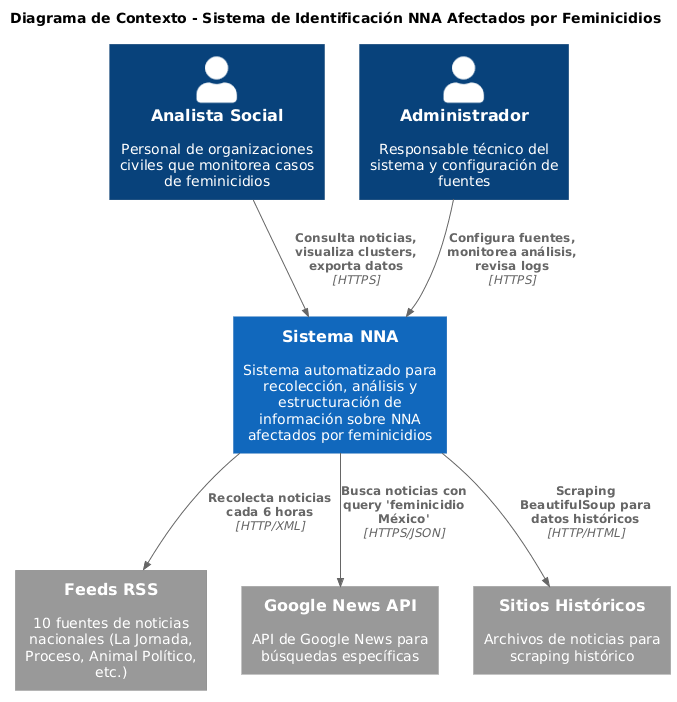
\includegraphics[width=0.75\textwidth,keepaspectratio]{media/Diagrama_contexto.png}
\caption{Diagrama de contexto del sistema}
\label{fig:diagrama_contexto}
\end{figure}

\subsection{Diagrama de Casos de Uso}
\label{anexo:diagrama_casos_uso}

Este diagrama representa los casos de uso principales del sistema y las interacciones de los usuarios con el mismo.

\begin{figure}[h]
\centering
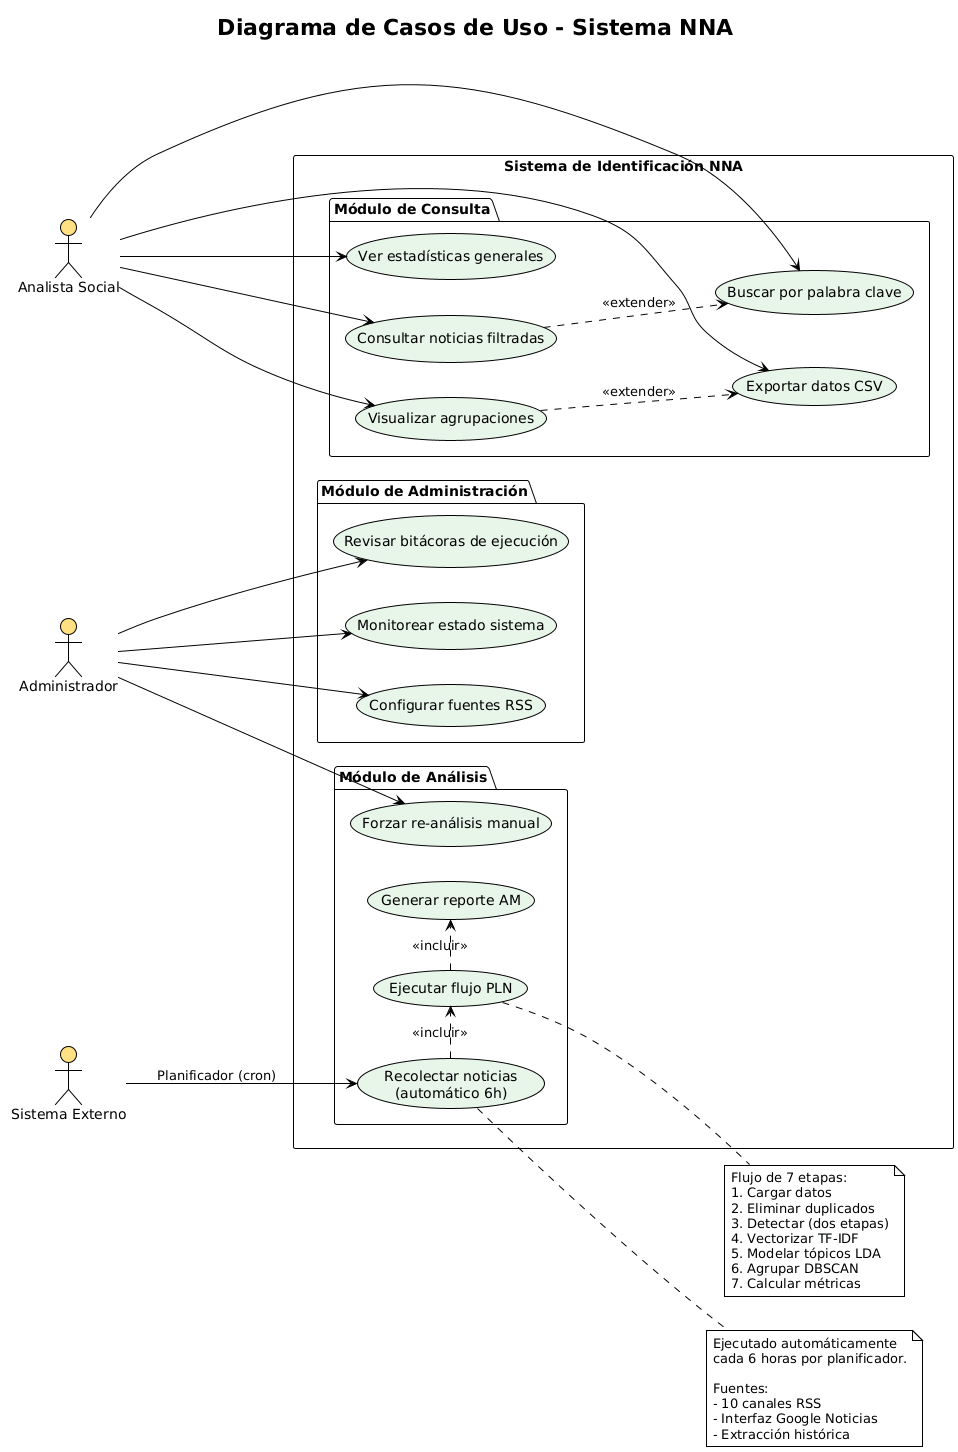
\includegraphics[width=0.75\textwidth,keepaspectratio]{media/Diagrama_casosUsos.png}
\caption{Diagrama de casos de uso del sistema}
\label{fig:diagrama_casos_uso}
\end{figure}

\subsection{Diagrama de Componentes}
\label{anexo:diagrama_componentes}

El diagrama de componentes muestra la estructura modular del sistema y las relaciones entre sus componentes principales.

\begin{figure}[h]
\centering
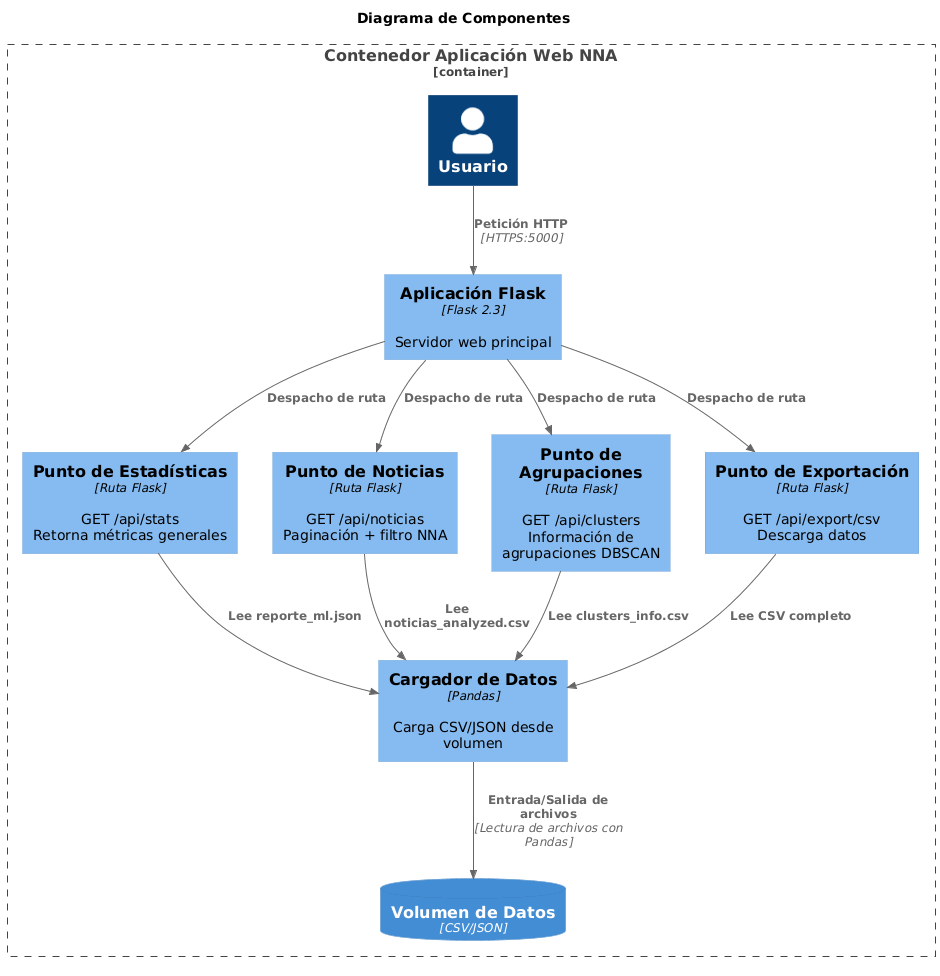
\includegraphics[width=0.75\textwidth,keepaspectratio]{media/Diagrama_componentes.png}
\caption{Diagrama de componentes del sistema}
\label{fig:diagrama_componentes}
\end{figure}

\subsection{Diagrama de Componentes de Análisis}
\label{anexo:diagrama_componentes_analisis}

Detalle de los componentes específicos del módulo de análisis de noticias.

\begin{figure}[p]
\centering
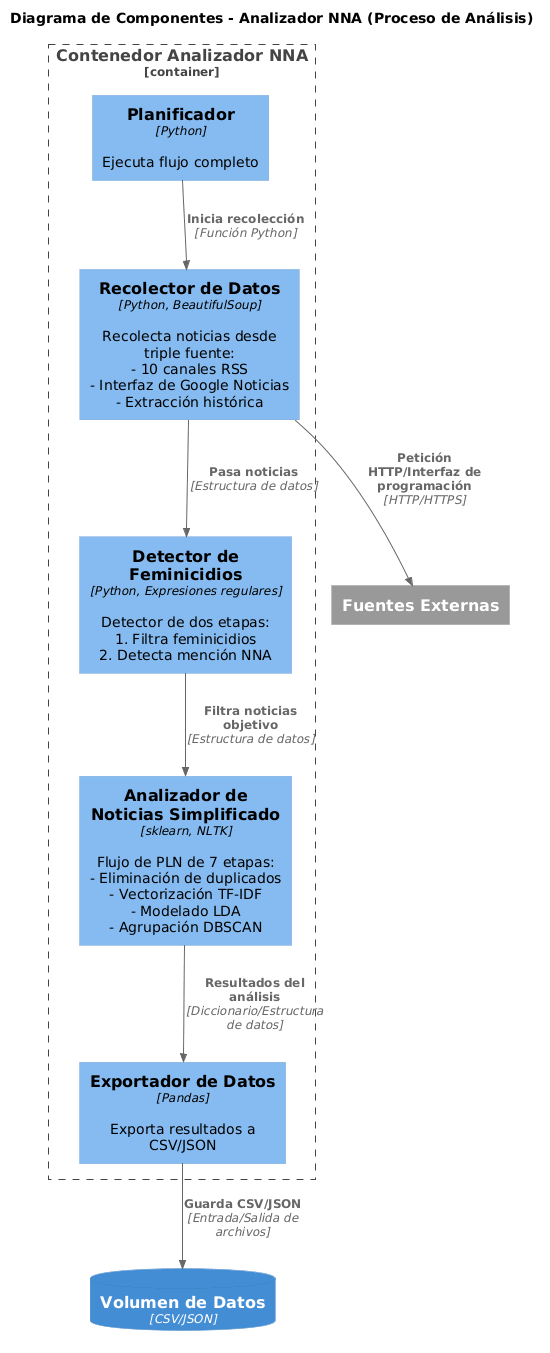
\includegraphics[height=0.85\textheight,keepaspectratio]{media/Diagrama_componentesAnalisis.png}
\caption{Diagrama de componentes del módulo de análisis}
\label{fig:diagrama_componentes_analisis}
\end{figure}

\clearpage

%----------------------------------------------------------------------------------------
% ANEXO B: DIAGRAMAS DE FLUJO Y PROCESOS
%----------------------------------------------------------------------------------------
\section{Diagramas de Flujo y Procesos}
\label{anexo:diagramas_flujo}

\subsection{Diagrama de Flujo Completo del Sistema}
\label{anexo:flujo_completo}

Este diagrama muestra el flujo completo de procesamiento de información en el sistema, desde la recolección hasta la presentación de resultados.

\begin{figure}[h]
\centering
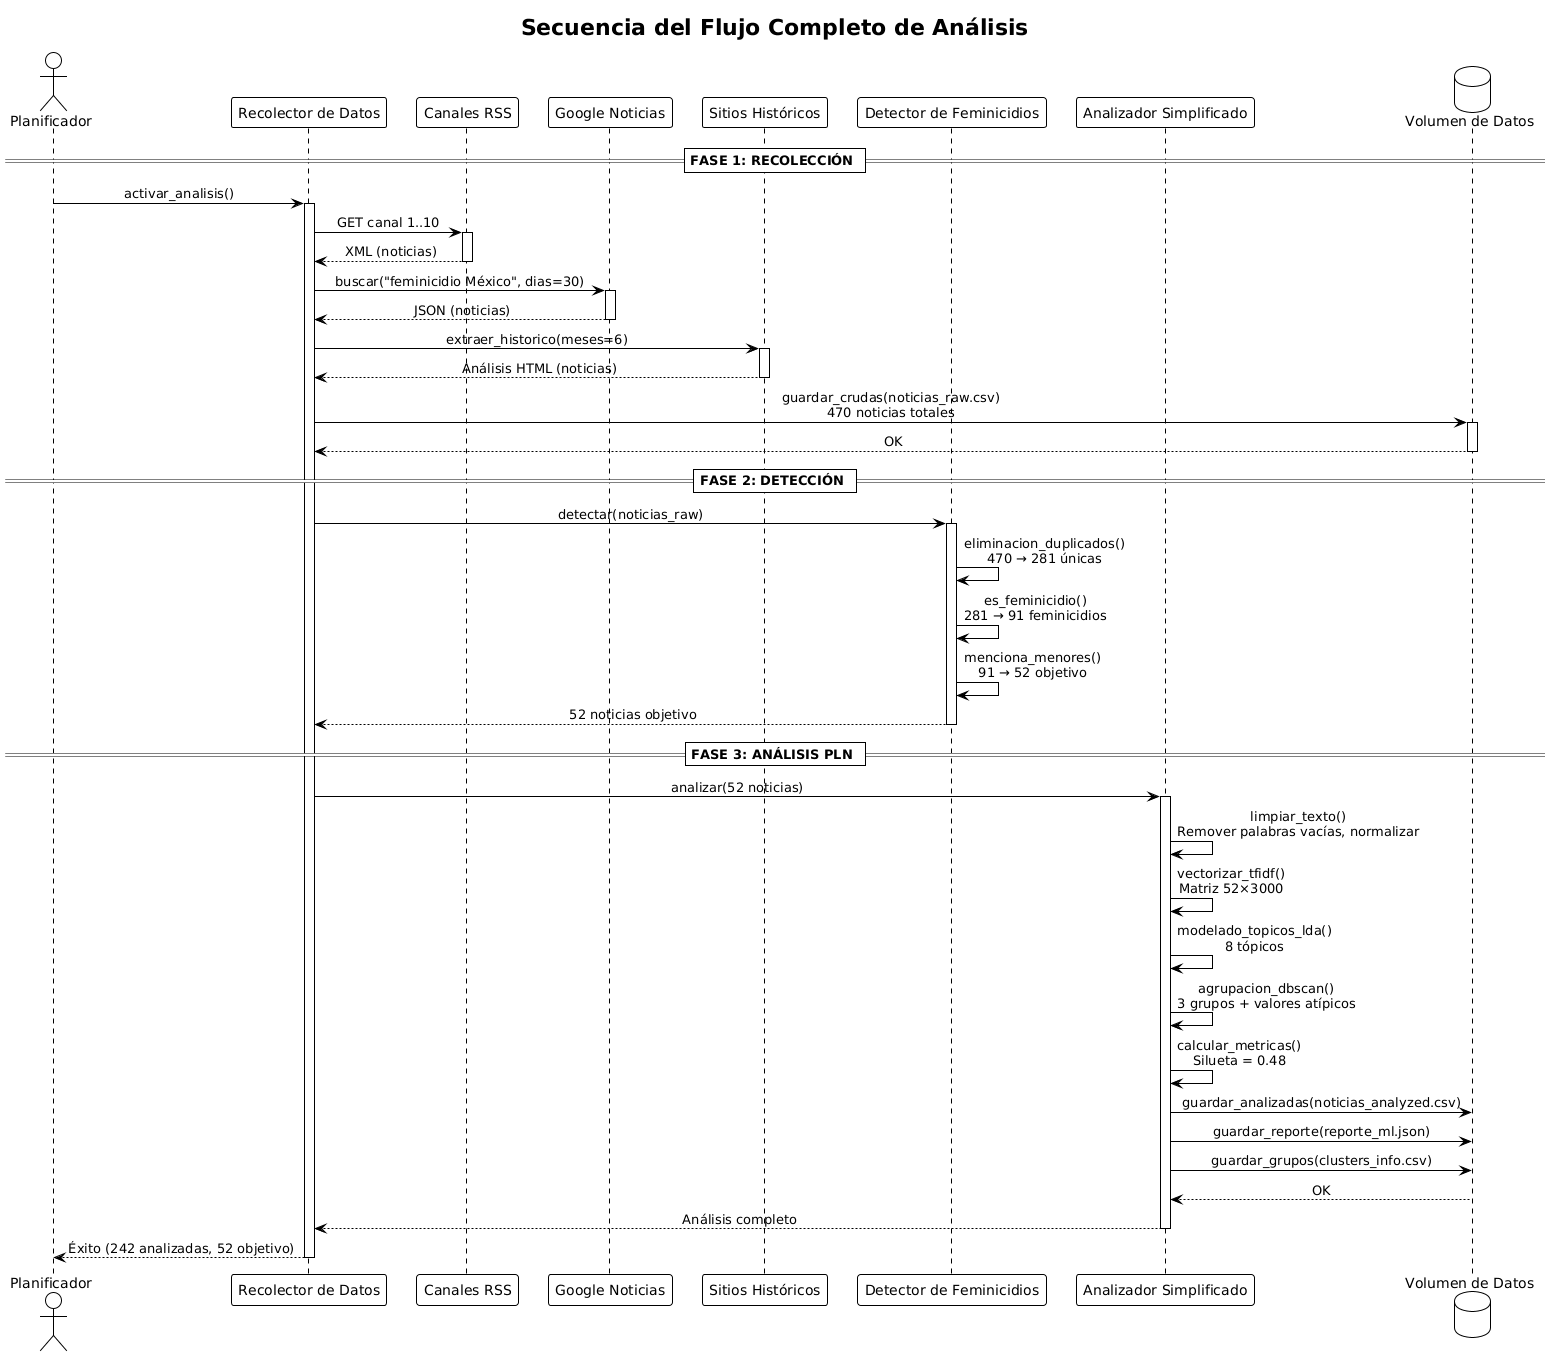
\includegraphics[width=0.7\textwidth,keepaspectratio]{media/Diagra_flujoCompleto.png}
\caption{Diagrama de flujo completo del sistema}
\label{fig:flujo_completo}
\end{figure}

\subsection{Diagrama de flujo de metodologías}
\label{anexo:flujo_pnl}

Detalle del flujo de las metodologías aplicadasa las noticias recolectadas.

\begin{figure}[p]
\centering
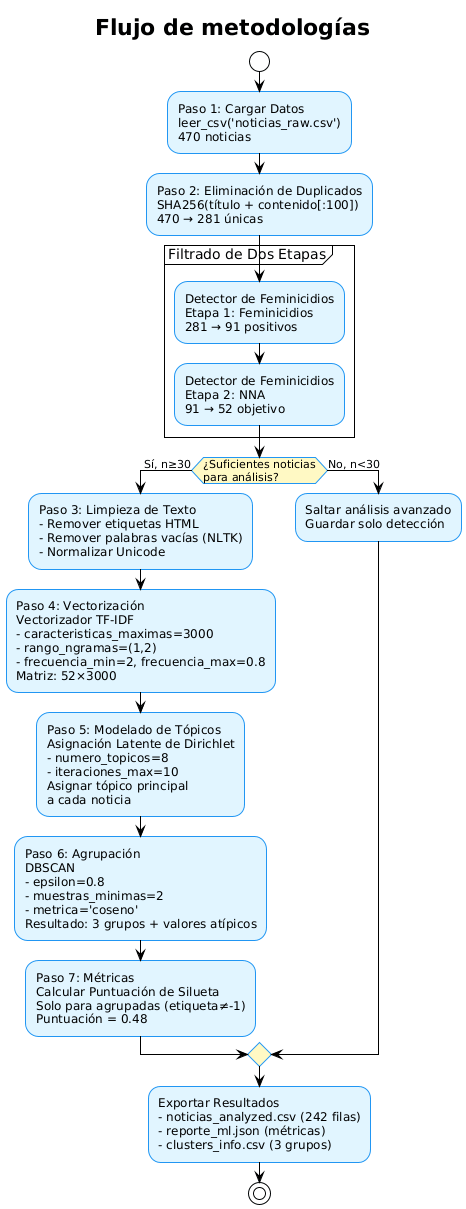
\includegraphics[height=0.85\textheight,keepaspectratio]{media/Diagrama_flujoPNL.png}
\caption{Diagrama de flujo de metodologías}
\label{fig:flujo_pnl}
\end{figure}

\subsection{Diagrama del Detector de Dos Etapas}
\label{anexo:detector_dos_etapas}

Diagrama que ilustra el funcionamiento del detector especializado de feminicidios con menciones de NNA, implementado en dos etapas para reducir falsos positivos.

\begin{figure}[h]
\centering
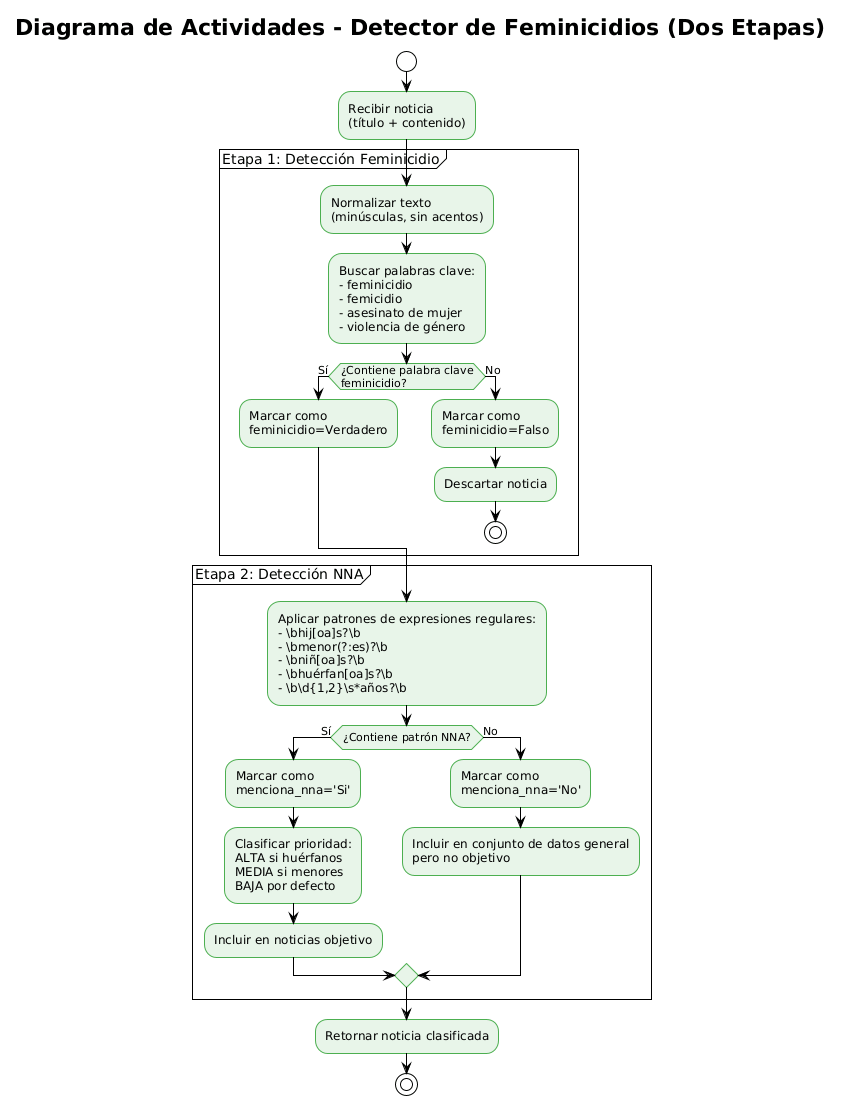
\includegraphics[width=0.7\textwidth,keepaspectratio]{media/Diagrama_detectorDosEtapas.png}
\caption{Diagrama del detector de feminicidios en dos etapas}
\label{fig:detector_dos_etapas}
\end{figure}

\clearpage

%----------------------------------------------------------------------------------------
% ANEXO C: ARQUITECTURA DOCKER Y EVOLUCIÓN
%----------------------------------------------------------------------------------------
\section{Arquitectura de Contenedores y Evolución del Sistema}
\label{anexo:docker_evolucion}

\subsection{Arquitectura Docker}
\label{anexo:arquitectura_docker}

Diagrama de la arquitectura de contenedores Docker implementada para el despliegue del sistema.

\begin{figure}[h]
\centering
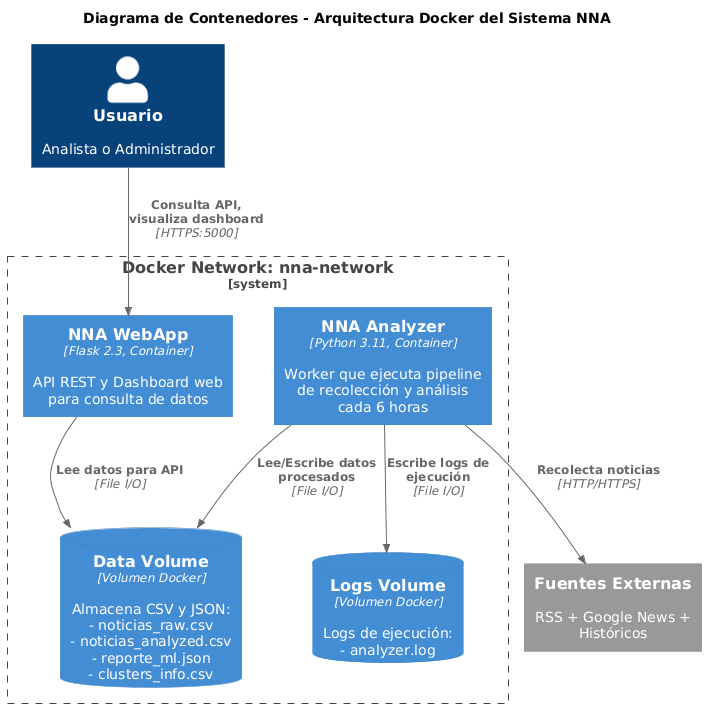
\includegraphics[width=0.75\textwidth,keepaspectratio]{media/Diagrama_docker.png}
\caption{Arquitectura Docker del sistema}
\label{fig:arquitectura_docker}
\end{figure}

\subsection{Evolución de Prototipos}
\label{anexo:evolucion_prototipos}

Diagrama que muestra la evolución del sistema a través de los diferentes prototipos desarrollados (P0, P1, P2).

\begin{figure}[h]
\centering
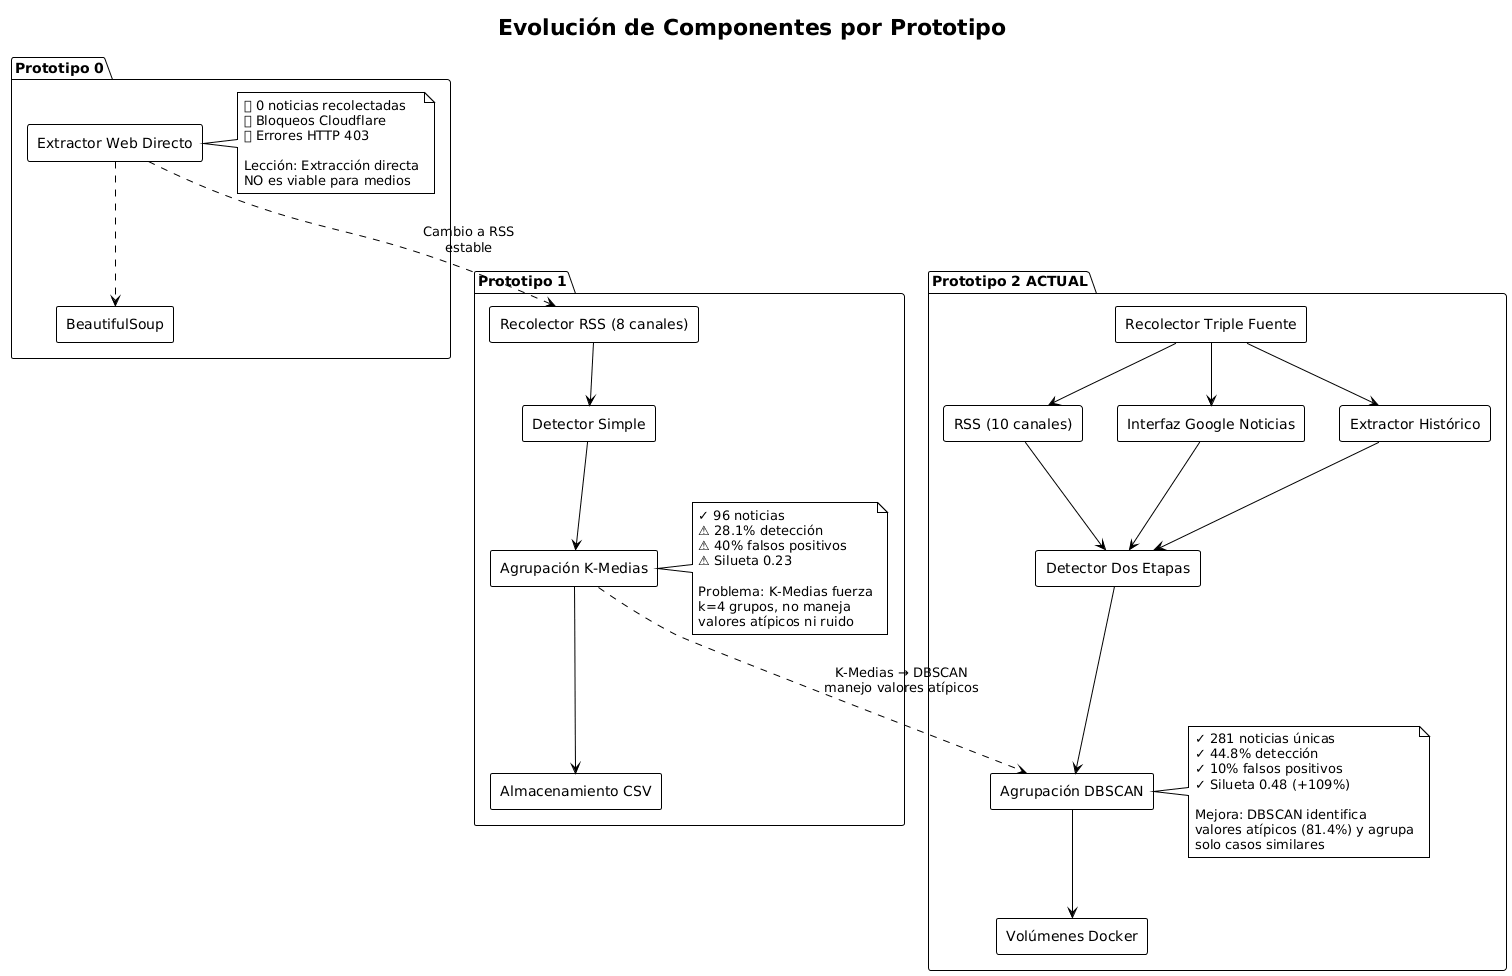
\includegraphics[width=0.75\textwidth,keepaspectratio]{media/Diagrama_evolucion.png}
\caption{Evolución de prototipos del sistema}
\label{fig:evolucion_prototipos}
\end{figure}

\clearpage

%----------------------------------------------------------------------------------------
% ANEXO D: MOCKUPS DE INTERFAZ DE USUARIO
%----------------------------------------------------------------------------------------
\section{Mockups de Interfaz de Usuario}
\label{anexo:mockups}

Esta sección presenta los diseños de interfaz de usuario del sistema.

\subsection{Mockup de Pantalla de Login}
\label{anexo:mockup_login}

Diseño de la pantalla de inicio de sesión del sistema.

\begin{figure}[h]
\centering
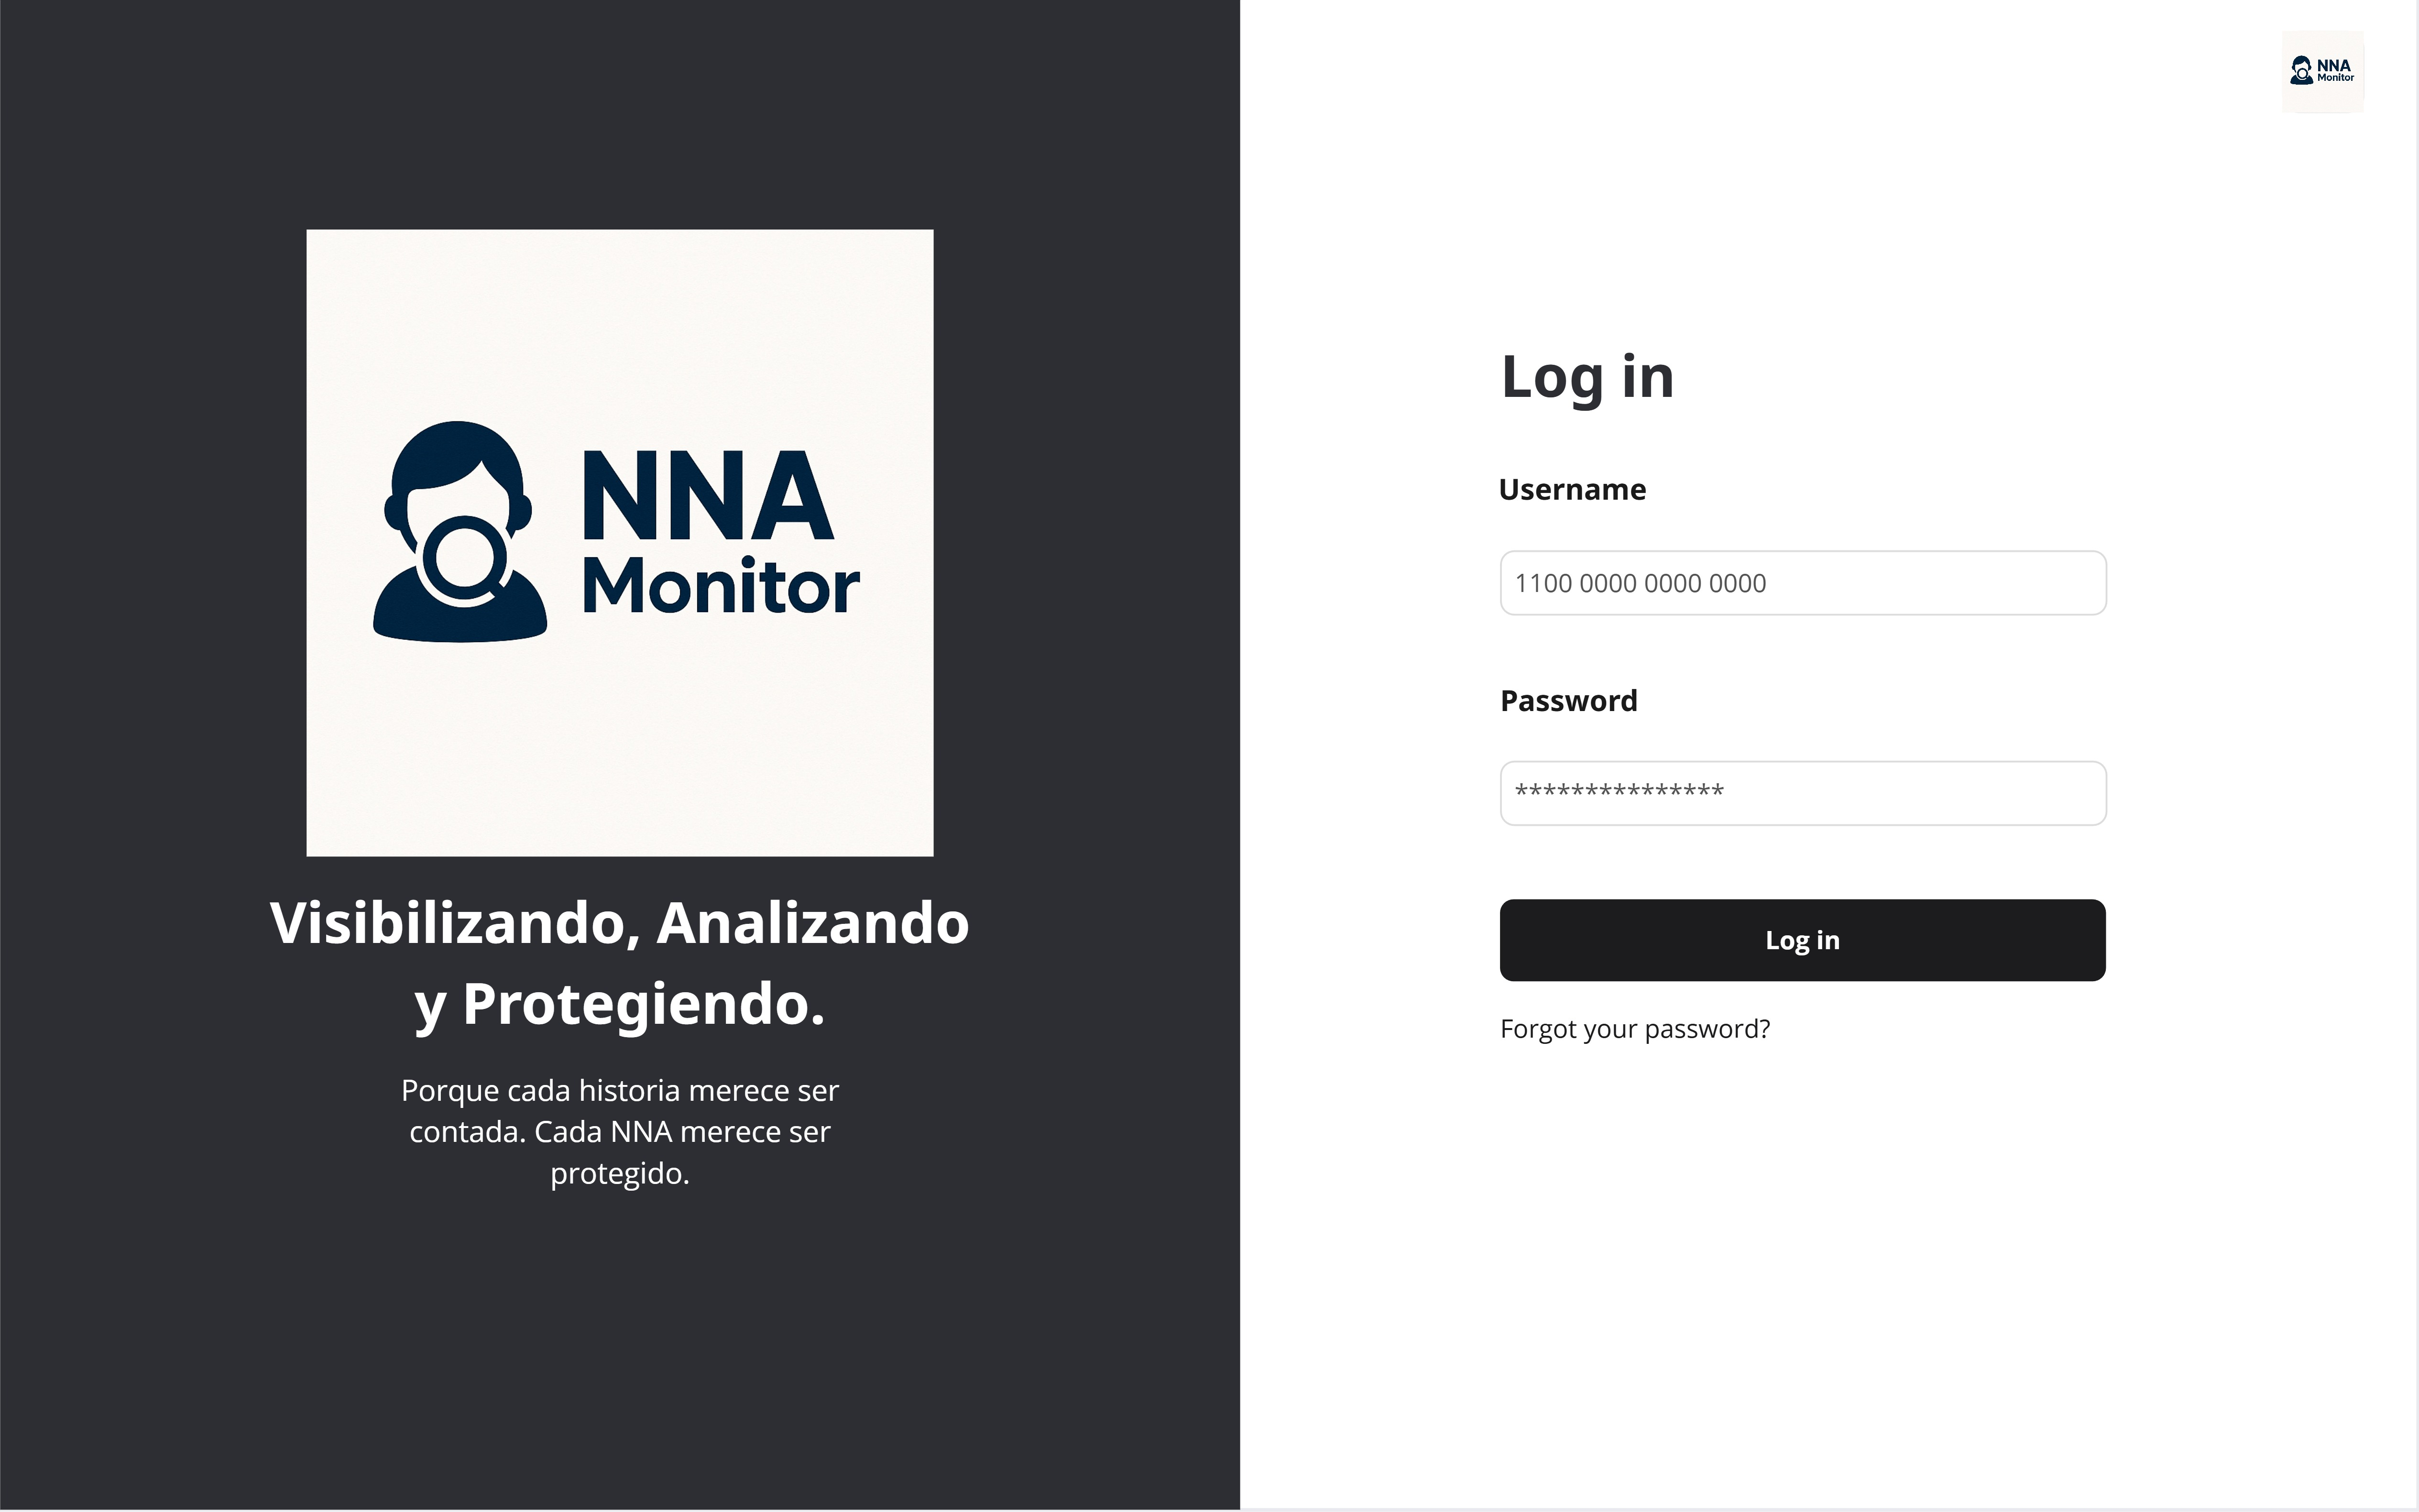
\includegraphics[width=0.7\textwidth,keepaspectratio]{media/Mockup_login.jpg}
\caption{Mockup de la pantalla de login}
\label{fig:mockup_login}
\end{figure}

\subsection{Mockup de Pantalla Principal (Home)}
\label{anexo:mockup_home}

Diseño de la pantalla principal del sistema donde se visualiza el dashboard con la información general.

\begin{figure}[h]
\centering
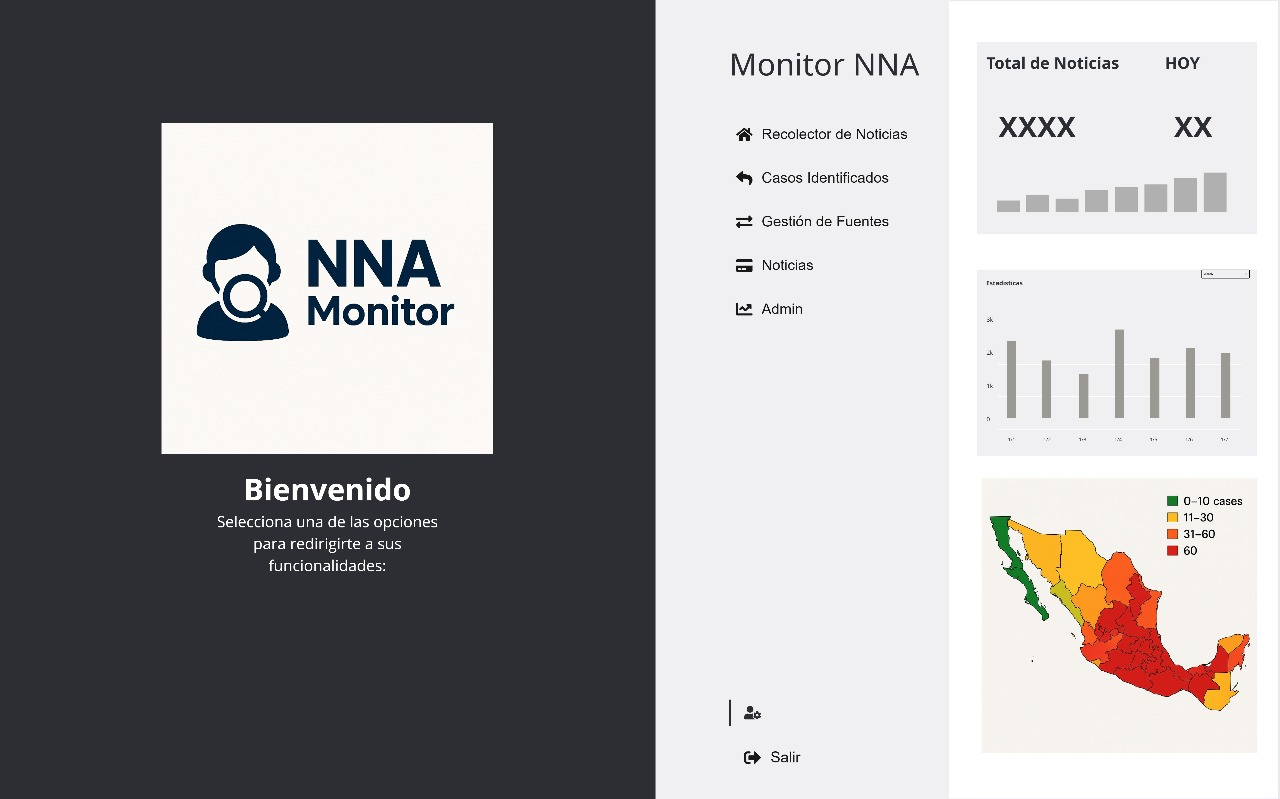
\includegraphics[width=0.7\textwidth,keepaspectratio]{media/Mockup_home.jpg}
\caption{Mockup de la pantalla principal (Home)}
\label{fig:mockup_home}
\end{figure}

\subsection{Mockup de Resumen General}
\label{anexo:mockup_resumen}

Diseño de la pantalla de resumen general con estadísticas y métricas del sistema.

\begin{figure}[h]
\centering
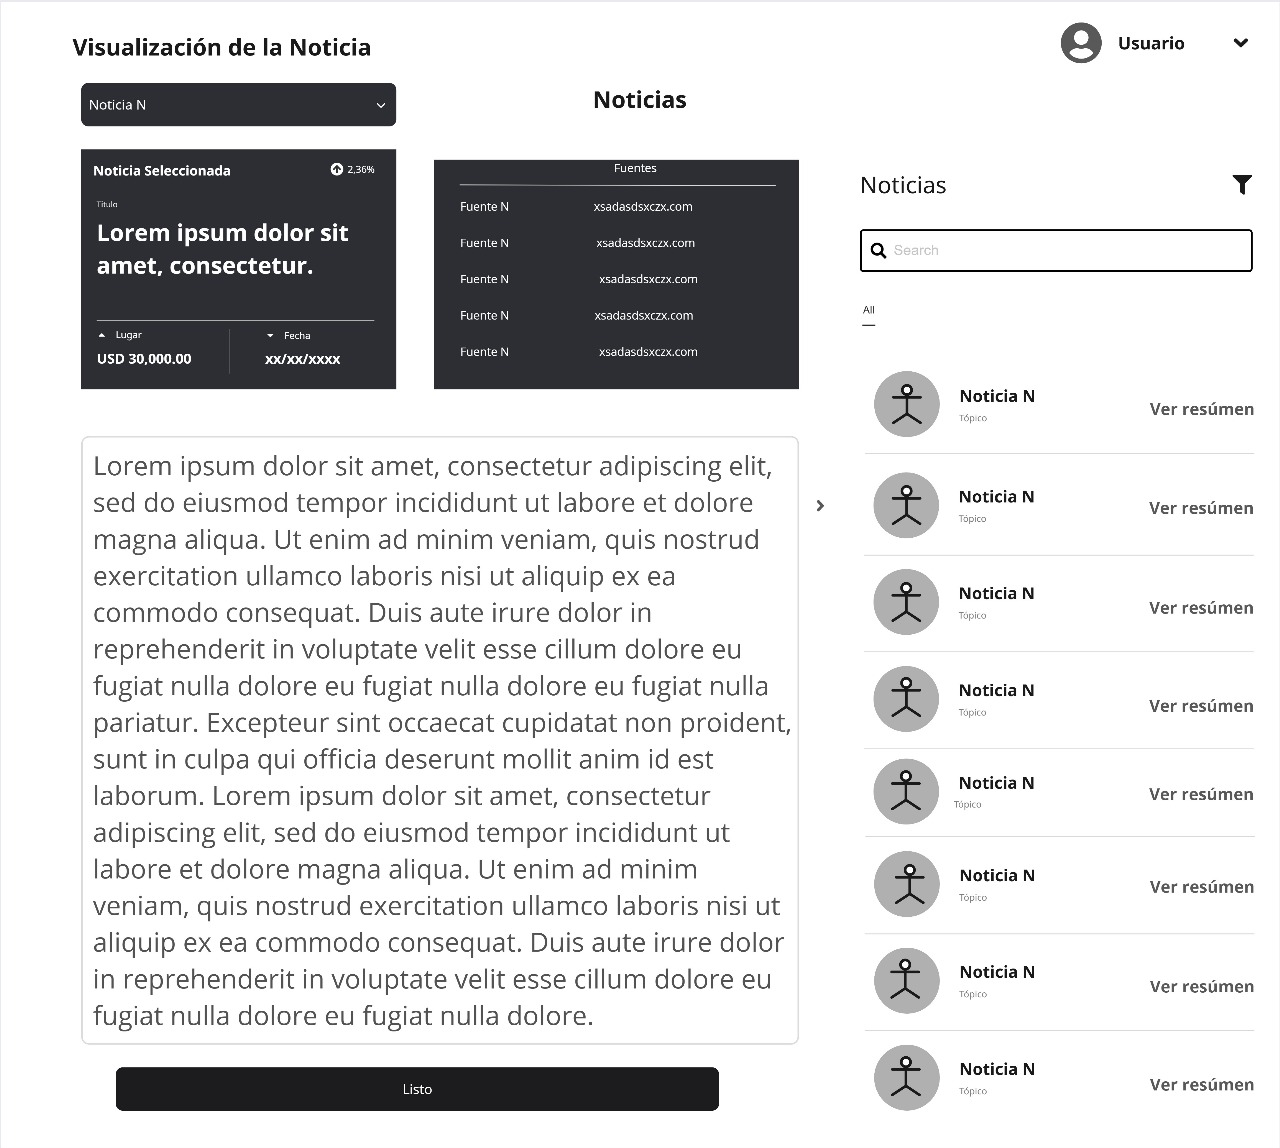
\includegraphics[width=0.7\textwidth,keepaspectratio]{media/Mockup_ResumenGeneral.jpg}
\caption{Mockup de la pantalla de resumen general}
\label{fig:mockup_resumen}
\end{figure}

\clearpage

\subsection{Mockup de Recolector de Noticias}
\label{anexo:mockup_recolector}

Diseño de la interfaz del módulo de recolección de noticias.

\begin{figure}[h]
\centering
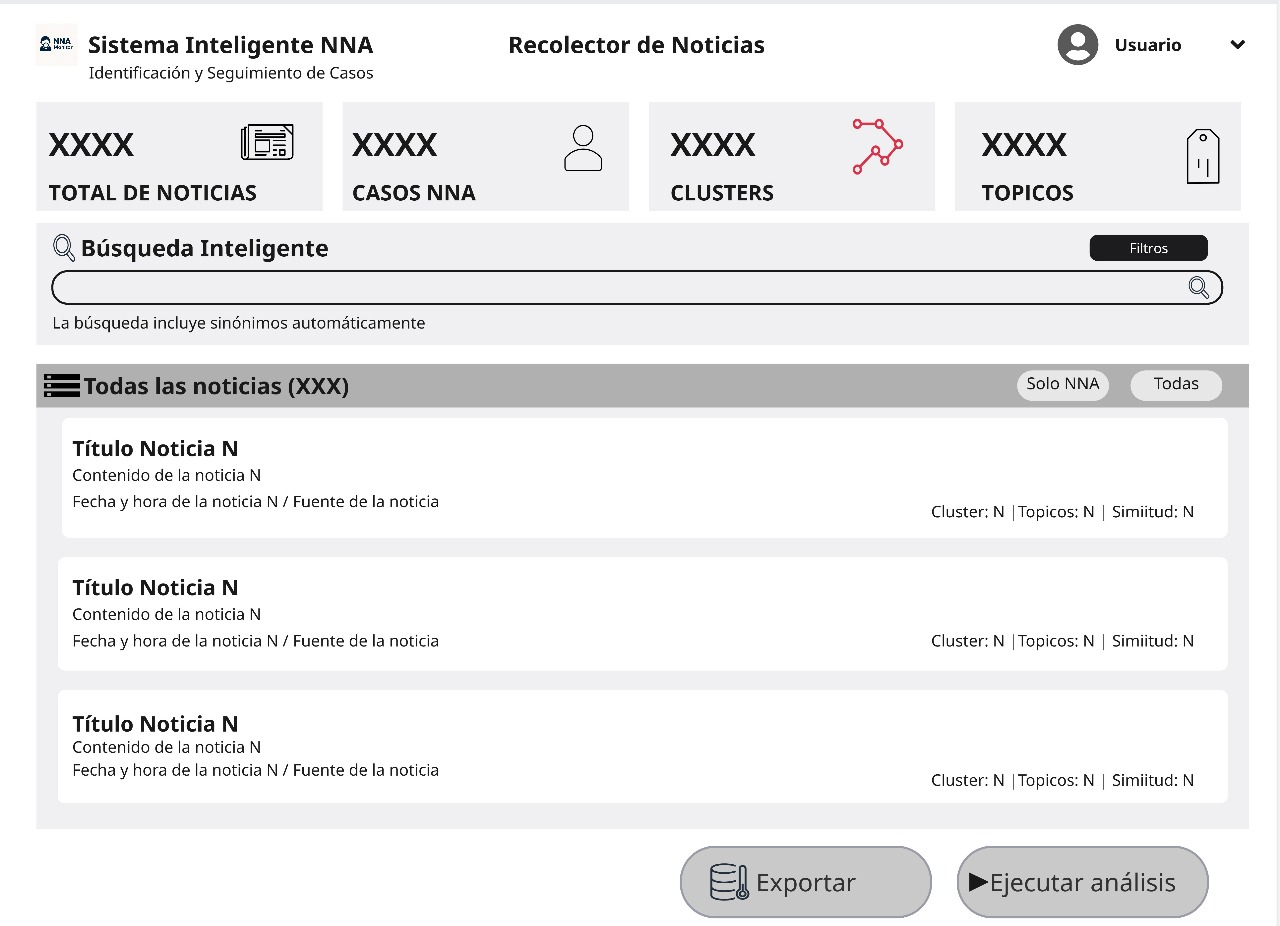
\includegraphics[width=0.7\textwidth,keepaspectratio]{media/Mockup_RecolectorNoticias.jpg}
\caption{Mockup del recolector de noticias}
\label{fig:mockup_recolector}
\end{figure}

\subsection{Mockup de Gestión de Fuentes}
\label{anexo:mockup_fuentes}

Diseño de la pantalla de gestión y configuración de fuentes de información.

\begin{figure}[h]
\centering
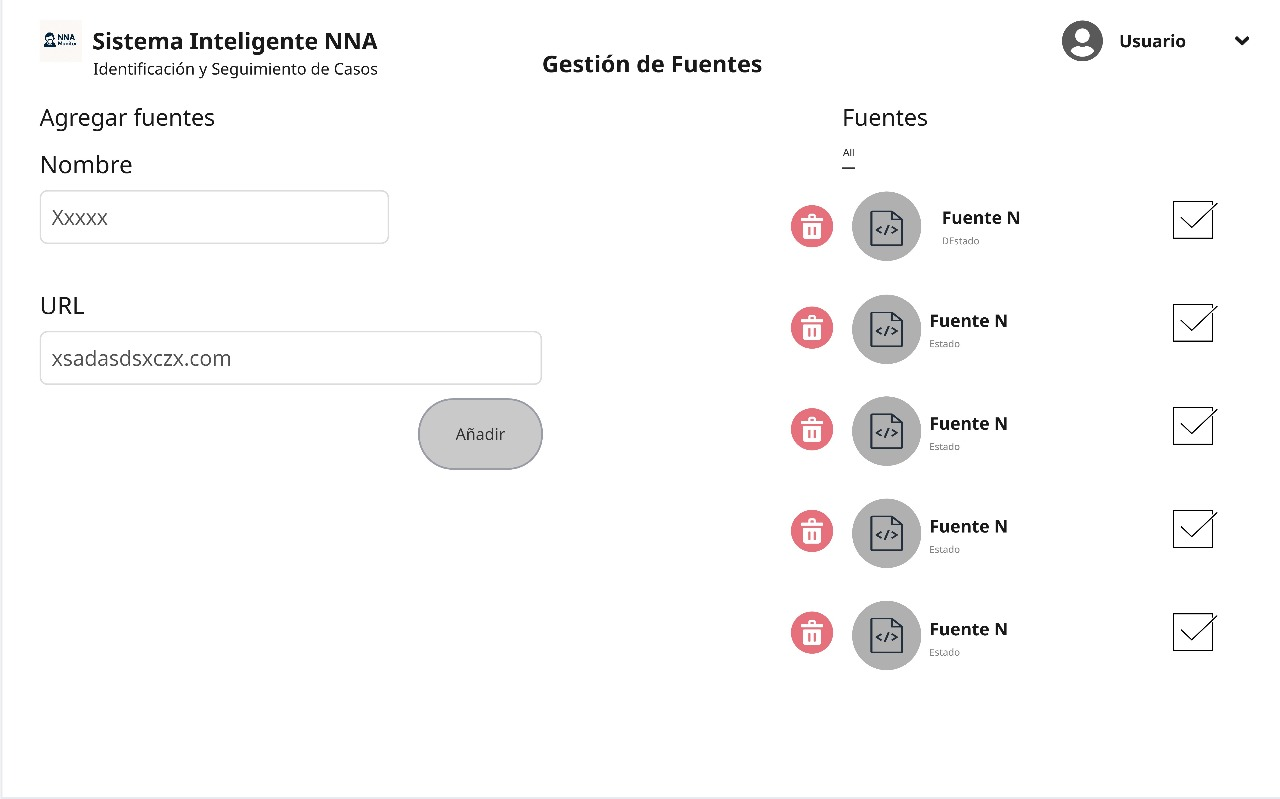
\includegraphics[width=0.7\textwidth,keepaspectratio]{media/Mockup_GestionFuentes.jpg}
\caption{Mockup de gestión de fuentes}
\label{fig:mockup_fuentes}
\end{figure}

\subsection{Mockup de Filtros}
\label{anexo:mockup_filtro}

Diseño de la interfaz de filtros para búsqueda y análisis de noticias.

\begin{figure}[h]
\centering
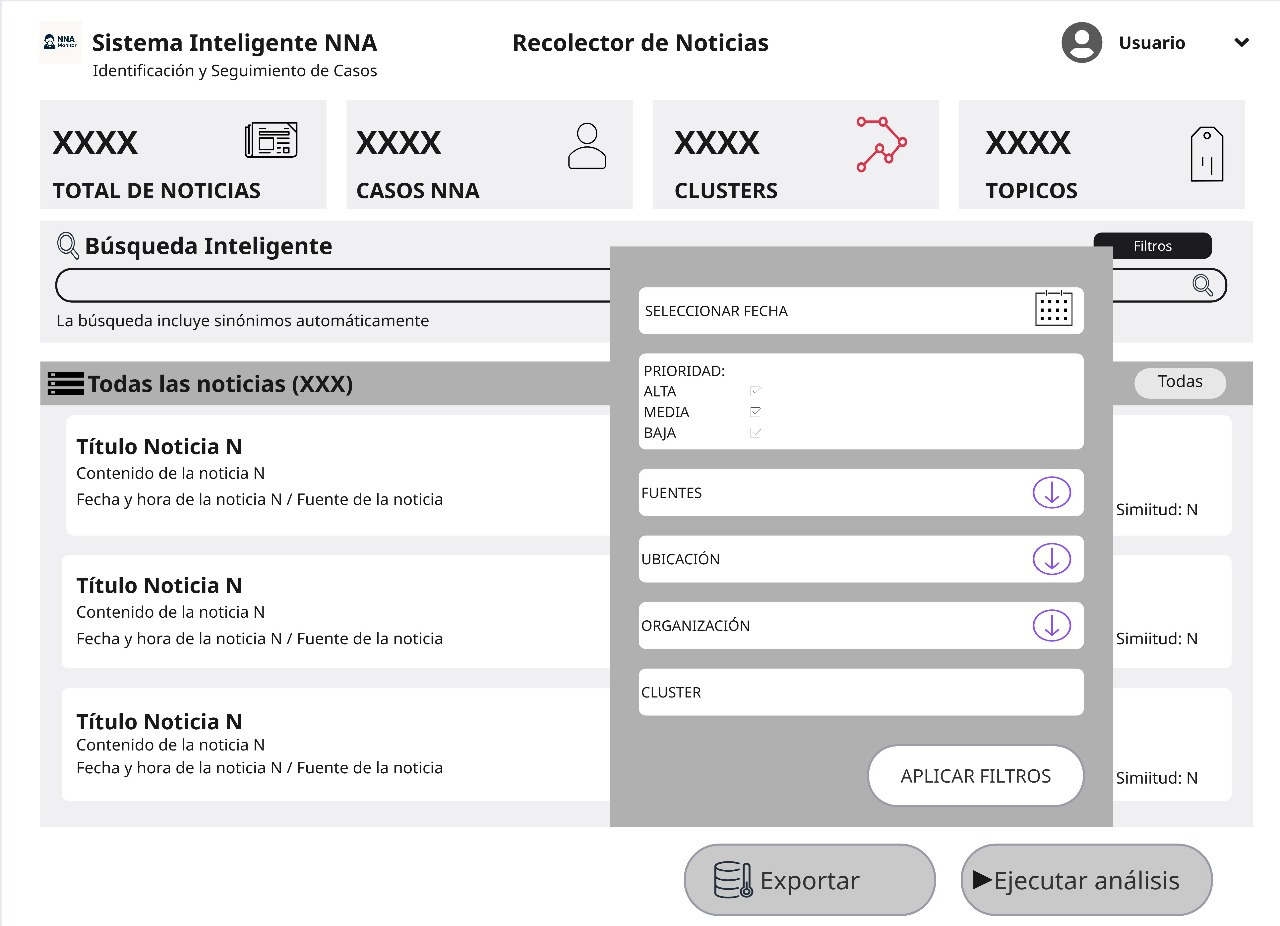
\includegraphics[width=0.7\textwidth,keepaspectratio]{media/Mockup_filtro.jpg}
\caption{Mockup de la pantalla de filtros}
\label{fig:mockup_filtro}
\end{figure}

\clearpage

\subsection{Mockup de Perfil de Usuario}
\label{anexo:mockup_perfil}

Diseño de la pantalla de perfil y configuración de usuario.

\begin{figure}[h]
\centering
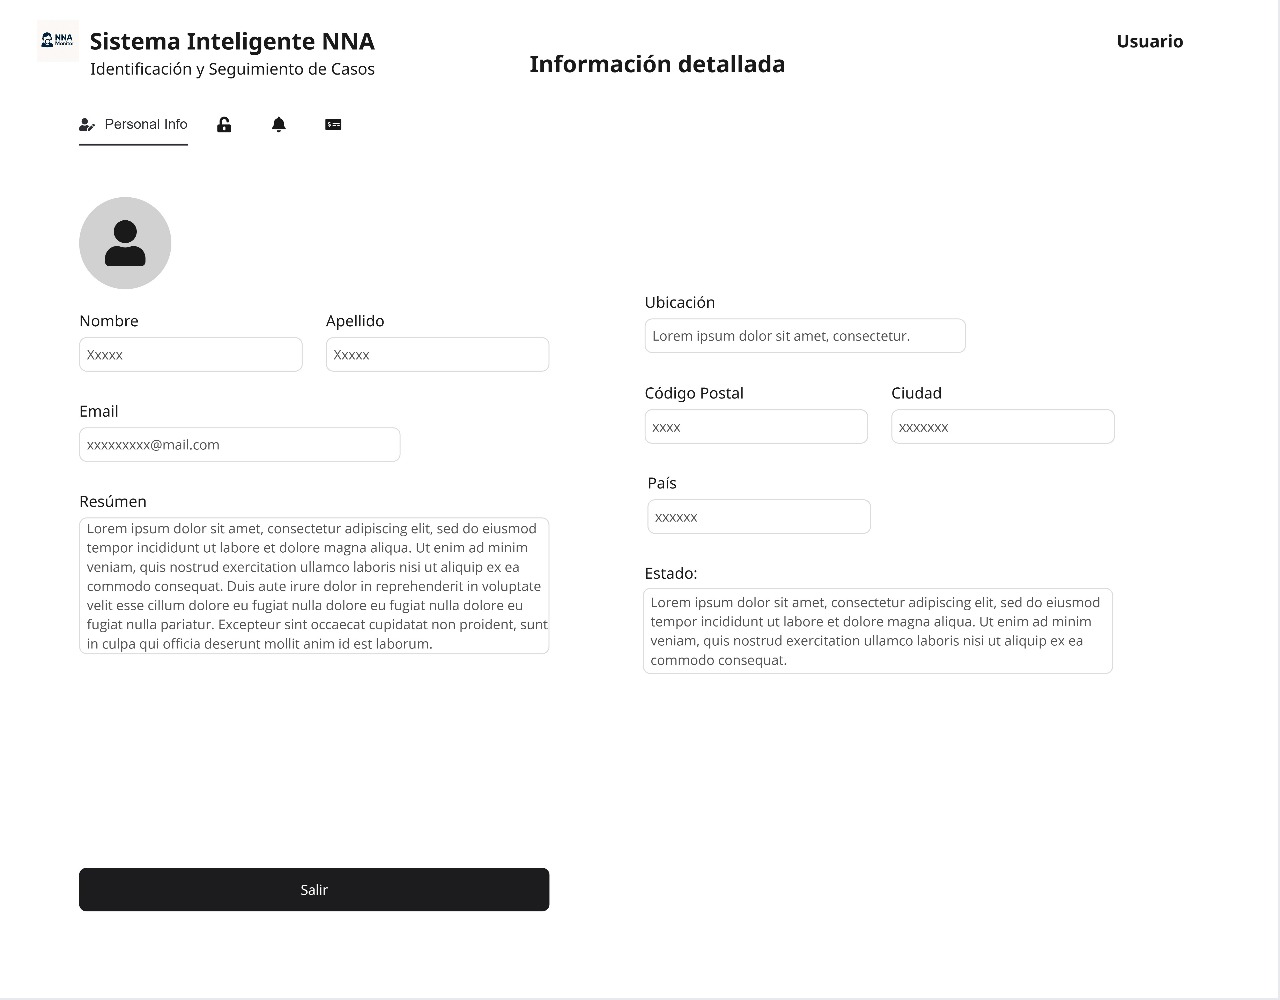
\includegraphics[width=0.7\textwidth,keepaspectratio]{media/Mockup_perfil.jpg}
\caption{Mockup del perfil de usuario}
\label{fig:mockup_perfil}
\end{figure}

\clearpage


\end{document}